\chapter{Machine learning analysis implementation}
\label{sec:MLanalysis}

In this chapter we are going to look at how the ML algorithms are implemented, trained and how they perform before we in the end are going to test it on real data. 

\section{Preparations and expectations}
For both machine learning algorithms, BDT and NN, we have done a few preselection cuts on the data before we feed it into our ML classifiers. It is necessary to make the datasets smaller in order to get a more reasonable training time and to avoid consuming too much memory when converting the input to dataframes\footnote{Pandas dataframes \cite{PD} is a two-dimensional frame of your data which also includes the corresponding labels.}. The cuts we have applied on the data are given in table \ref{tab:precutsSlepSlep} below.

\begin{table}[H]
    \centering
    \renewcommand{\arraystretch}{1.}
    \begin{tabular}{c}
    \toprule
    \textbf{Precuts}\\
    \midrule
    \midrule
        Number of leptons = 2 \\
        $E_T^{miss}$ $>$ 40 GeV\\
        \bottomrule
    \end{tabular}
    \caption{A table of the precuts we have done before sending the data into the BDT and NN.}
    \label{tab:precutsSlepSlep}
\end{table}

The features included, that is the kinematical variables, in the training of the ML algorithms have been selected using the different variables available in the MC nTuples\footnote{nTuple is the data format used in the high energy physics community to store large amounts of data for analysis within the framework known as ROOT \cite{root}.} and are listed in table \ref{tab:features}.

\begin{table}[H]
    \centering
    \renewcommand{\arraystretch}{1.}
    \begin{tabular}{c c}
    \toprule
    \textbf{Low level features} & \textbf{High level features}\\
    \midrule
    \midrule
        lep $p_{T_1}$ & mll\\
        lep $p_{T_2}$ & mt2\\
        lep $\eta_1$ & $H_T$\\
        lep $\eta_2$ & $E_T^{\text{miss}}/H_T$\\
        lep $\phi_1$ & $\Delta \phi(\Vec{p}_T^{ll}, E_T^{\text{miss}})$\\
        lep $\phi_2$ & $\Delta R_{ll}$\\
        nJet20 & Fractional $p_T$ difference\\
        nJet30\\
        n$_{\text{b-tagged jets}}$\\
        $E_T^{\text{miss}}$\\
        $E_T^{\text{miss}}$ significance\\
        Electric charge\\
        Flavor\\
        \bottomrule
    \end{tabular}
    \caption{List of features chosen for the training of the ML model, where high level features are more complicated kinematical variables than low.}
    \label{tab:features}
\end{table}

We have also included different variables to weight each event according to its cross-section, average number of collision per bunch crossing (pile--up) and other characteristic of the event. The weights are listed in table \ref{tab:eventWeights}.

\begin{table}[H]
    \centering
    \renewcommand{\arraystretch}{1.}
    \begin{tabular}{c}
    \toprule
    \textbf{Weights}\\
    \midrule
    \midrule
        event weight  \\
        pileup weight \\
        b-tag weight \\
        generator weight \\
        jvt weights (jet vertex tagger)\\
        global dilepton trigger SF (same flavor)\\
        Luminosity for MC 2015-2016 = 36.2 fb$^{-1}$\\
        Luminosity for MC 2017 = 44.3 fb$^{-1}$\\
        Luminosity for MC 2018 = 58.5 fb$^{-1}$\\
        \bottomrule
    \end{tabular}
    \caption{List of weights to weight each event in the dataframes and the luminosity for the data taken in 2015-2018.}
    \label{tab:eventWeights}
\end{table}

Figure \ref{fig:ML_cuts} shows the distribution of the variables/features for data, the simulated SM background and some selected new physics signal models. \improvement{Del opp figur så det ikke blir en hel tom side etter all tekst er helt ferdig.} Overall, it seems like there is good agreement between data and MC, except for some missing MC in the high MET tail (figure \ref{fig:metMLcuts} and \ref{fig:metSignMLcuts}) and high b-jet multiplicity (figure \ref{fig:bjetMLcuts}). Since it is overall good agreement we can trust the data we are putting into the ML.

\newgeometry{top=20mm, bottom=25mm, twoside,inner=3cm,outer=2cm}
\begin{figure}[H]
\centering
    \begin{subfigure}[t!]{0.49\textwidth}
        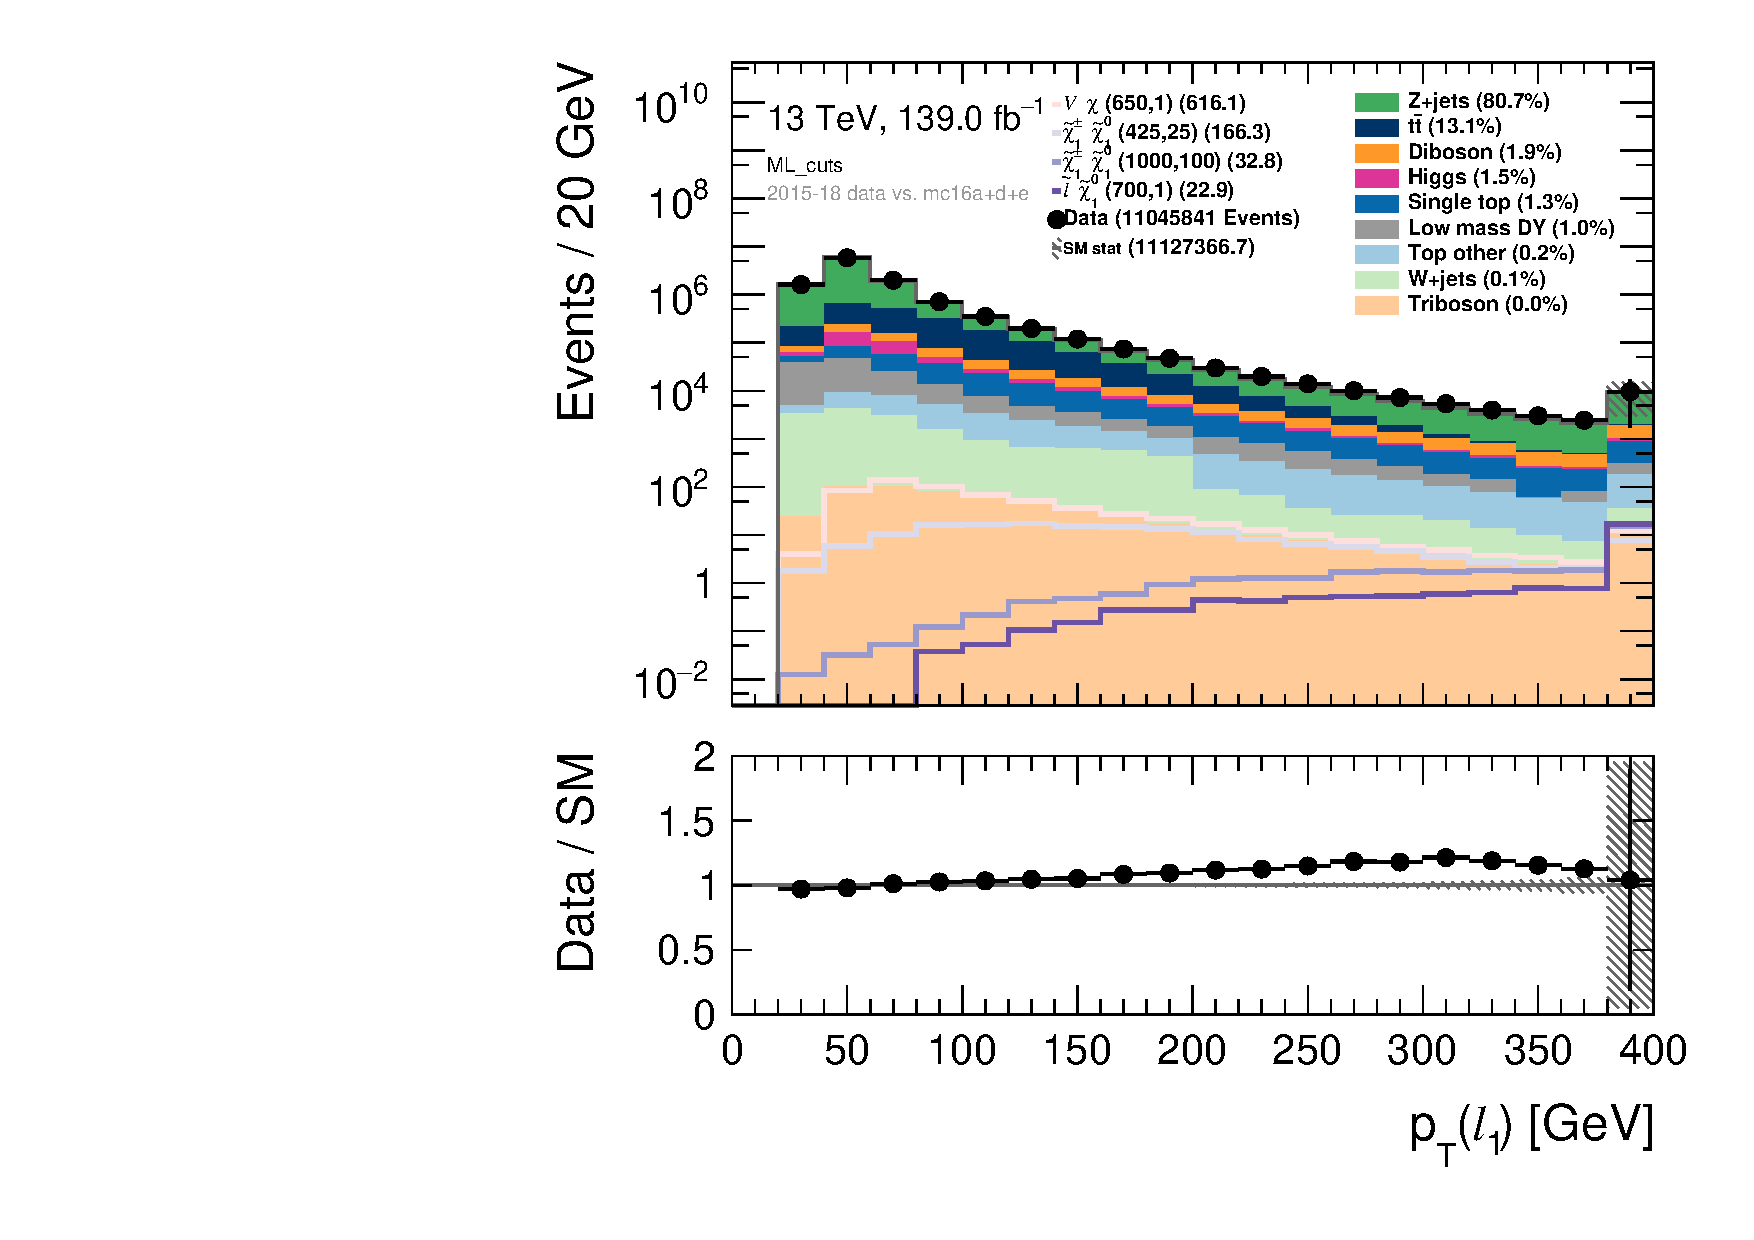
\includegraphics[width=\textwidth]{Figures/ML_cuts/hist1d_lepPt[0]_ML_cuts.pdf}
    \caption{The transverse momentum for lepton 1.}
    \label{fig:my_label}
    \end{subfigure}
    \begin{subfigure}[t!]{0.49\textwidth}
        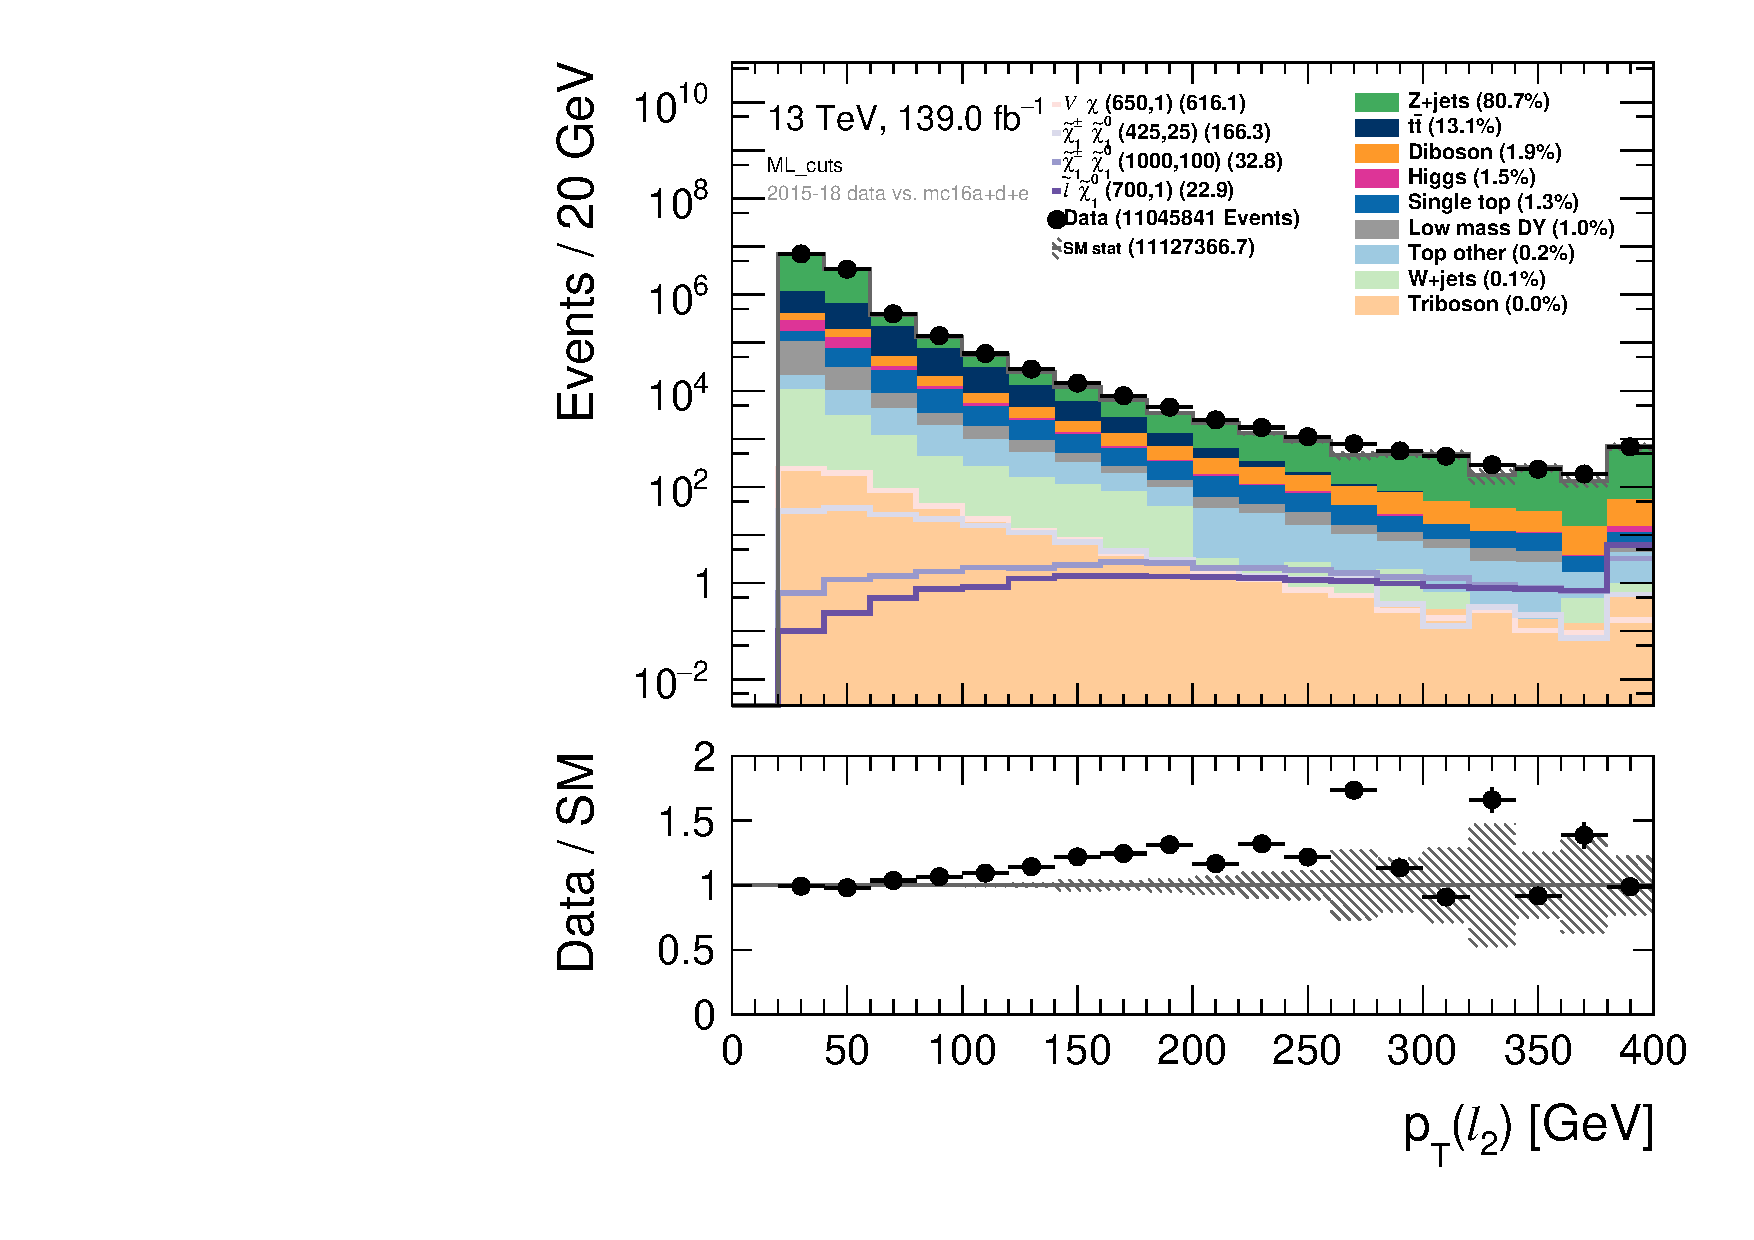
\includegraphics[width=\textwidth]{Figures/ML_cuts/hist1d_lepPt[1]_ML_cuts.pdf}
    \caption{Missing transverse energy.}
    \label{fig:my_label}
    \end{subfigure}
    \\
    \begin{subfigure}[t!]{0.49\textwidth}
        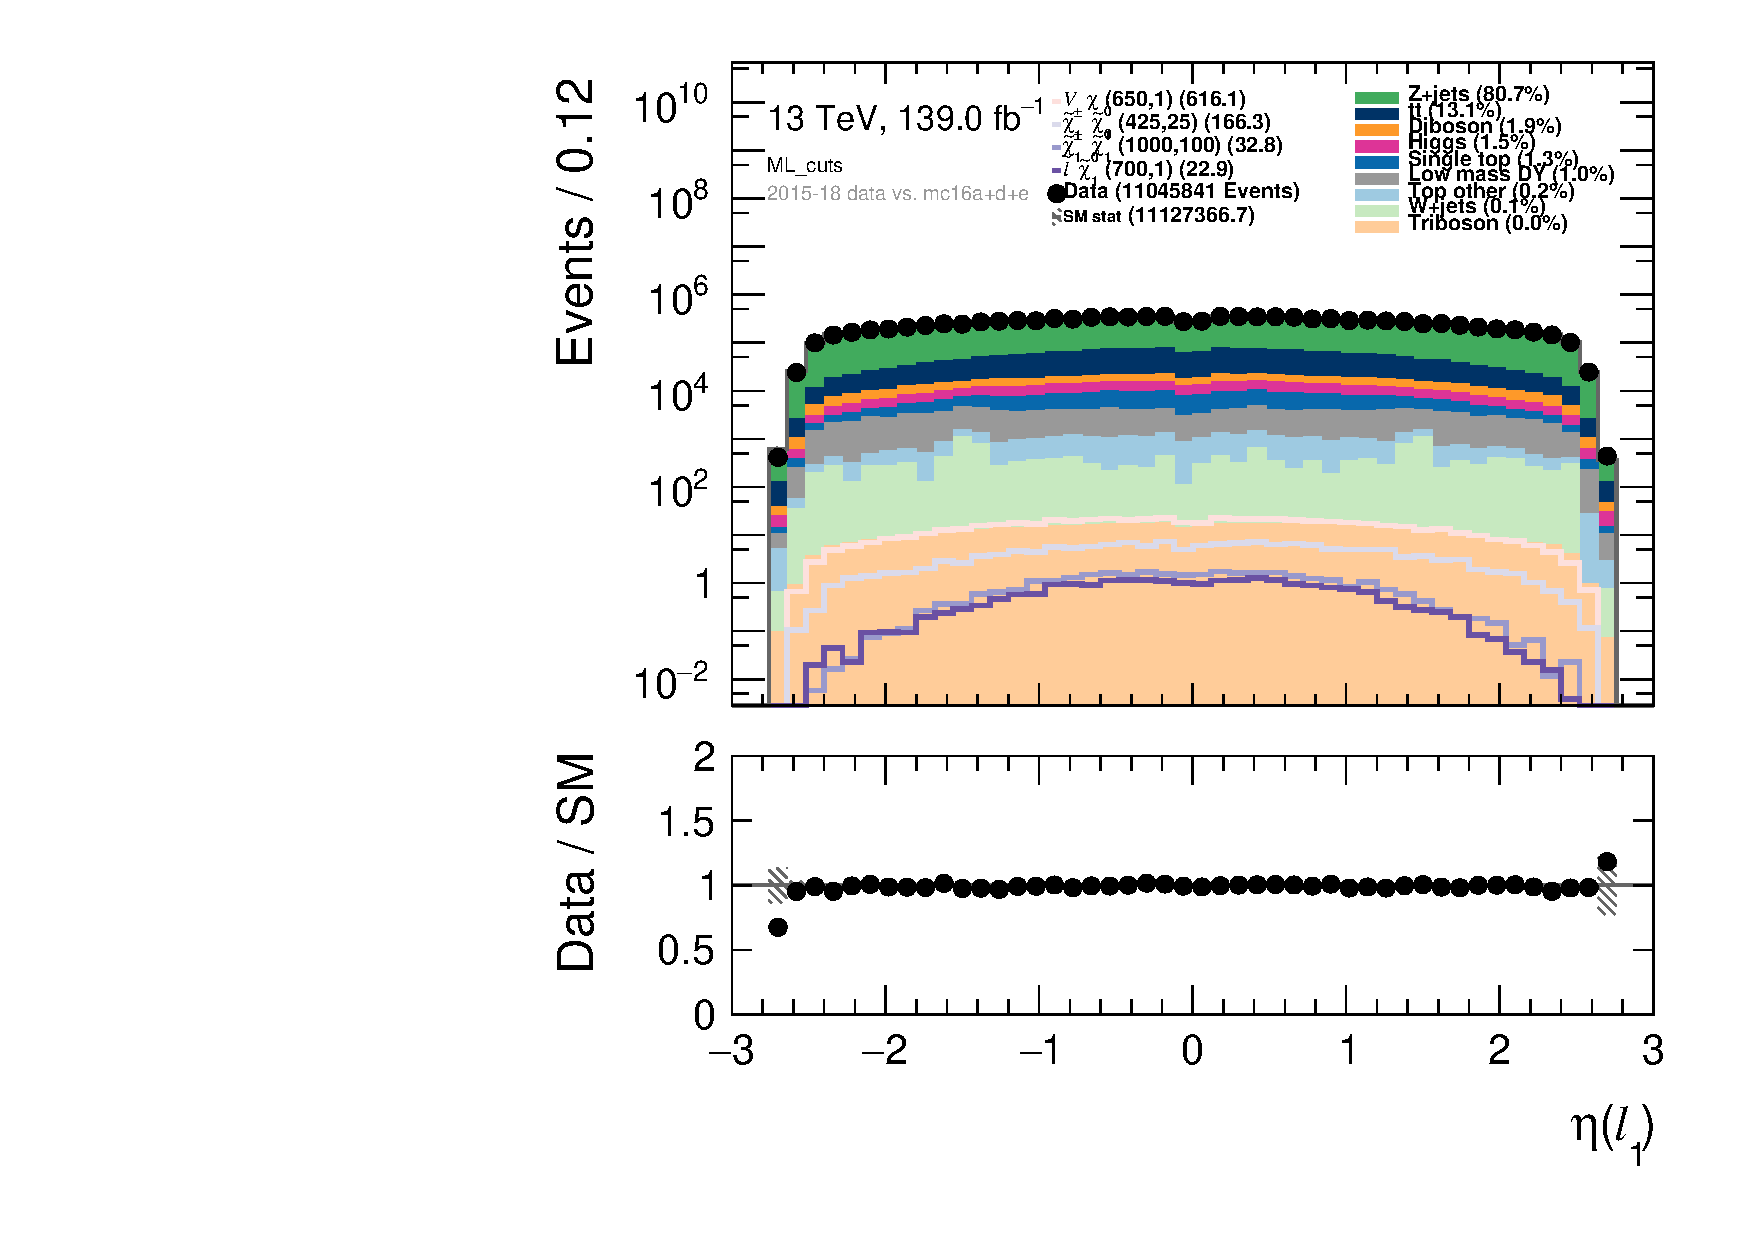
\includegraphics[width=\textwidth]{Figures/ML_cuts/hist1d_lepEta[0]_ML_cuts.pdf}
    \caption{The pseudorapidity for lepton 1.}
    \label{fig:my_label}
    \end{subfigure}
    \begin{subfigure}[t!]{0.49\textwidth}
        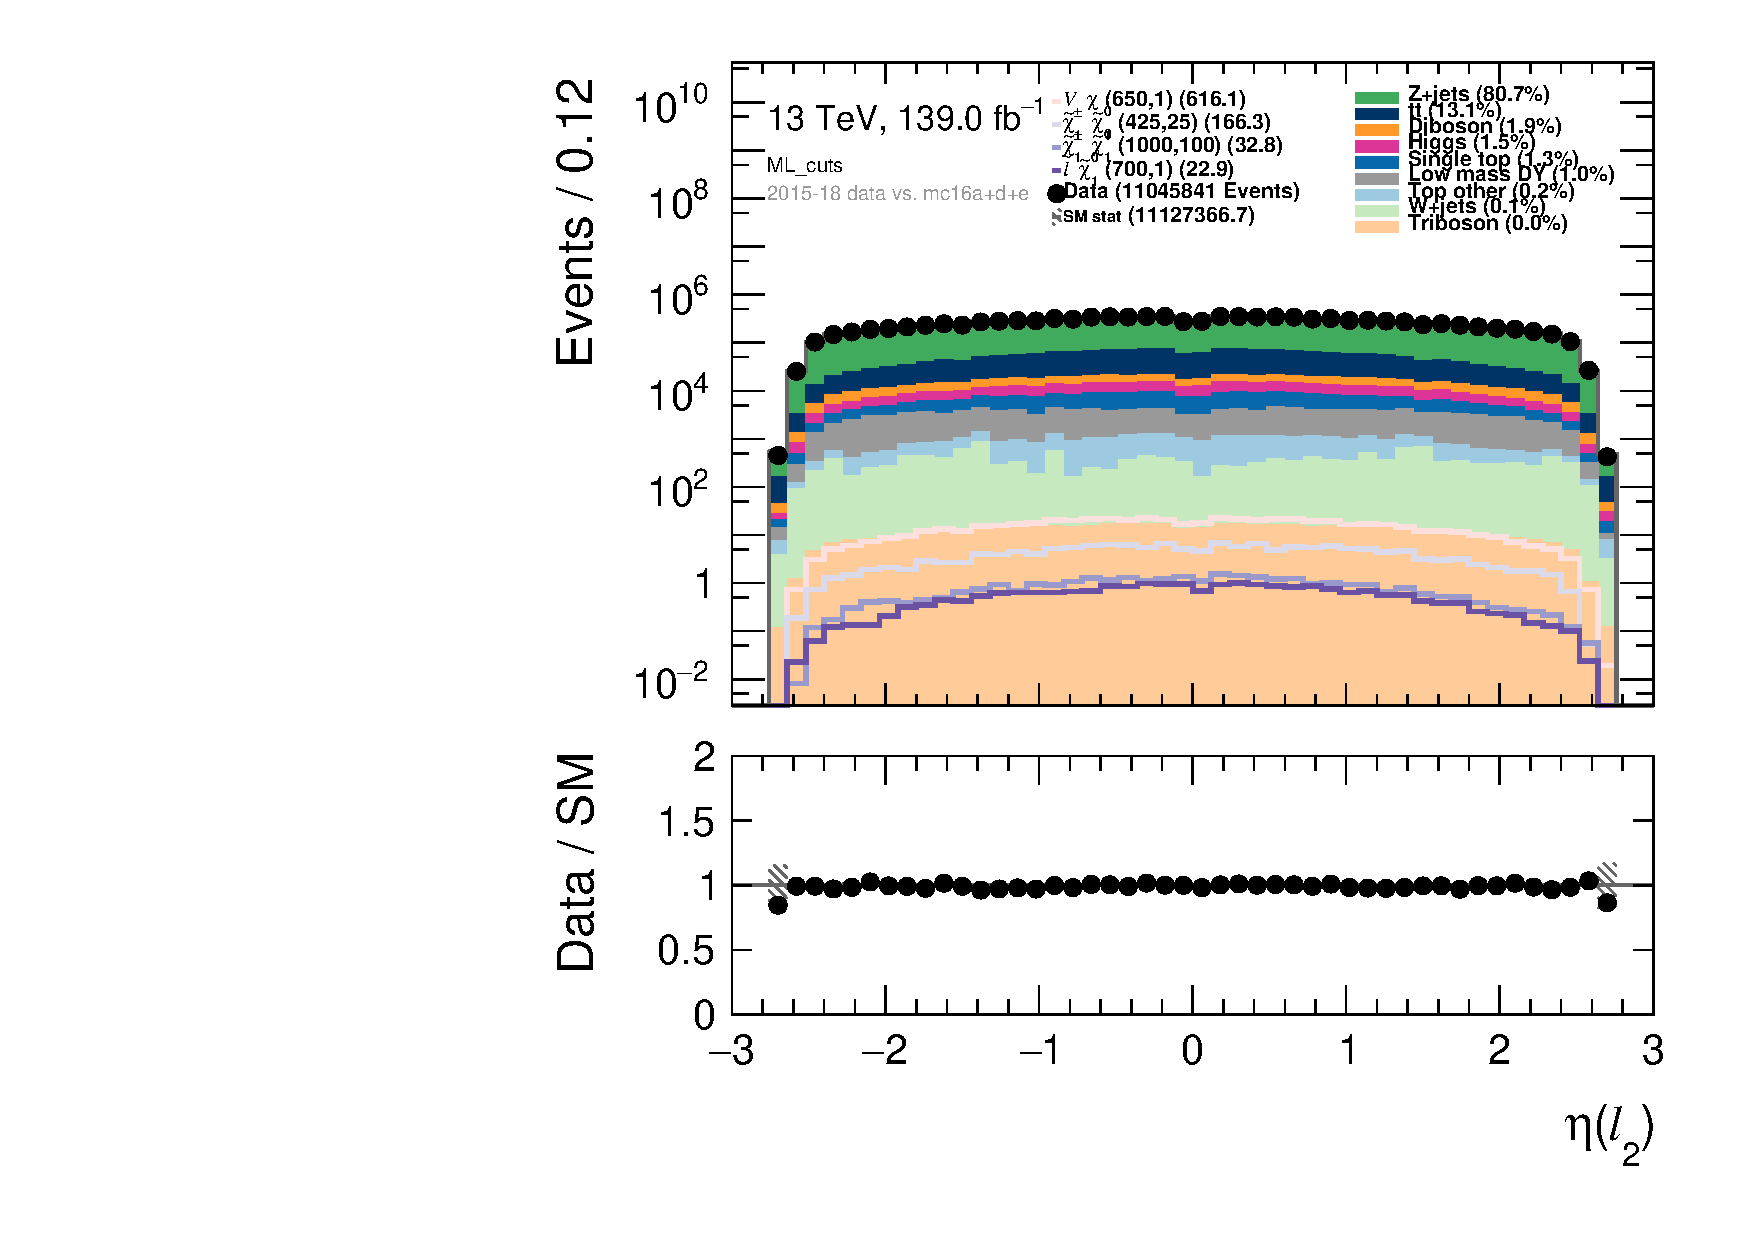
\includegraphics[width=\textwidth]{Figures/ML_cuts/hist1d_lepEta[1]_ML_cuts.pdf}
    \caption{The pseudorapidity for lepton 2.}
    \label{fig:my_label}
    \end{subfigure}
    \\
    \begin{subfigure}[t!]{0.49\textwidth}
        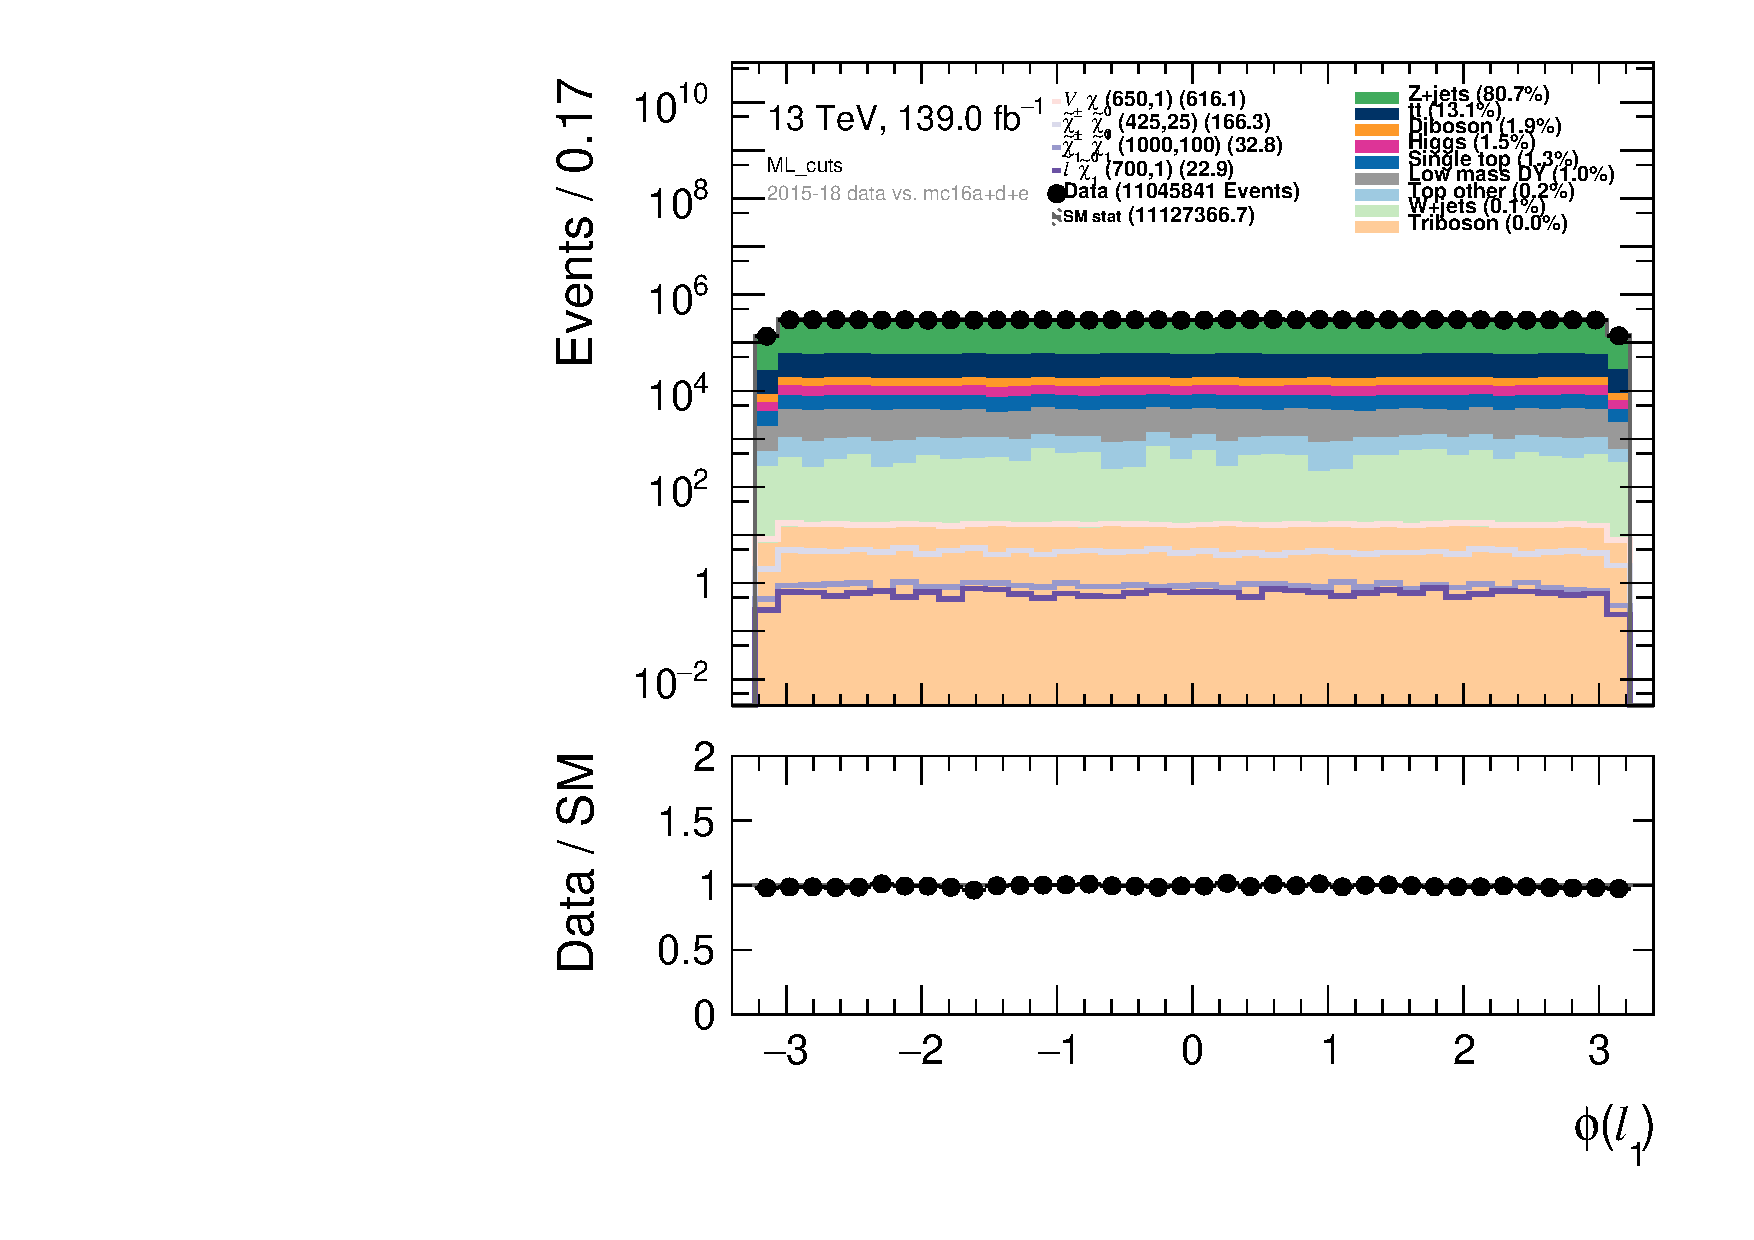
\includegraphics[width=\textwidth]{Figures/ML_cuts/hist1d_lepPhi[0]_ML_cuts.pdf}
    \caption{The azimuthal angle for lepton 1.}
    \label{fig:my_label}
    \end{subfigure}
    \begin{subfigure}[t!]{0.49\textwidth}
        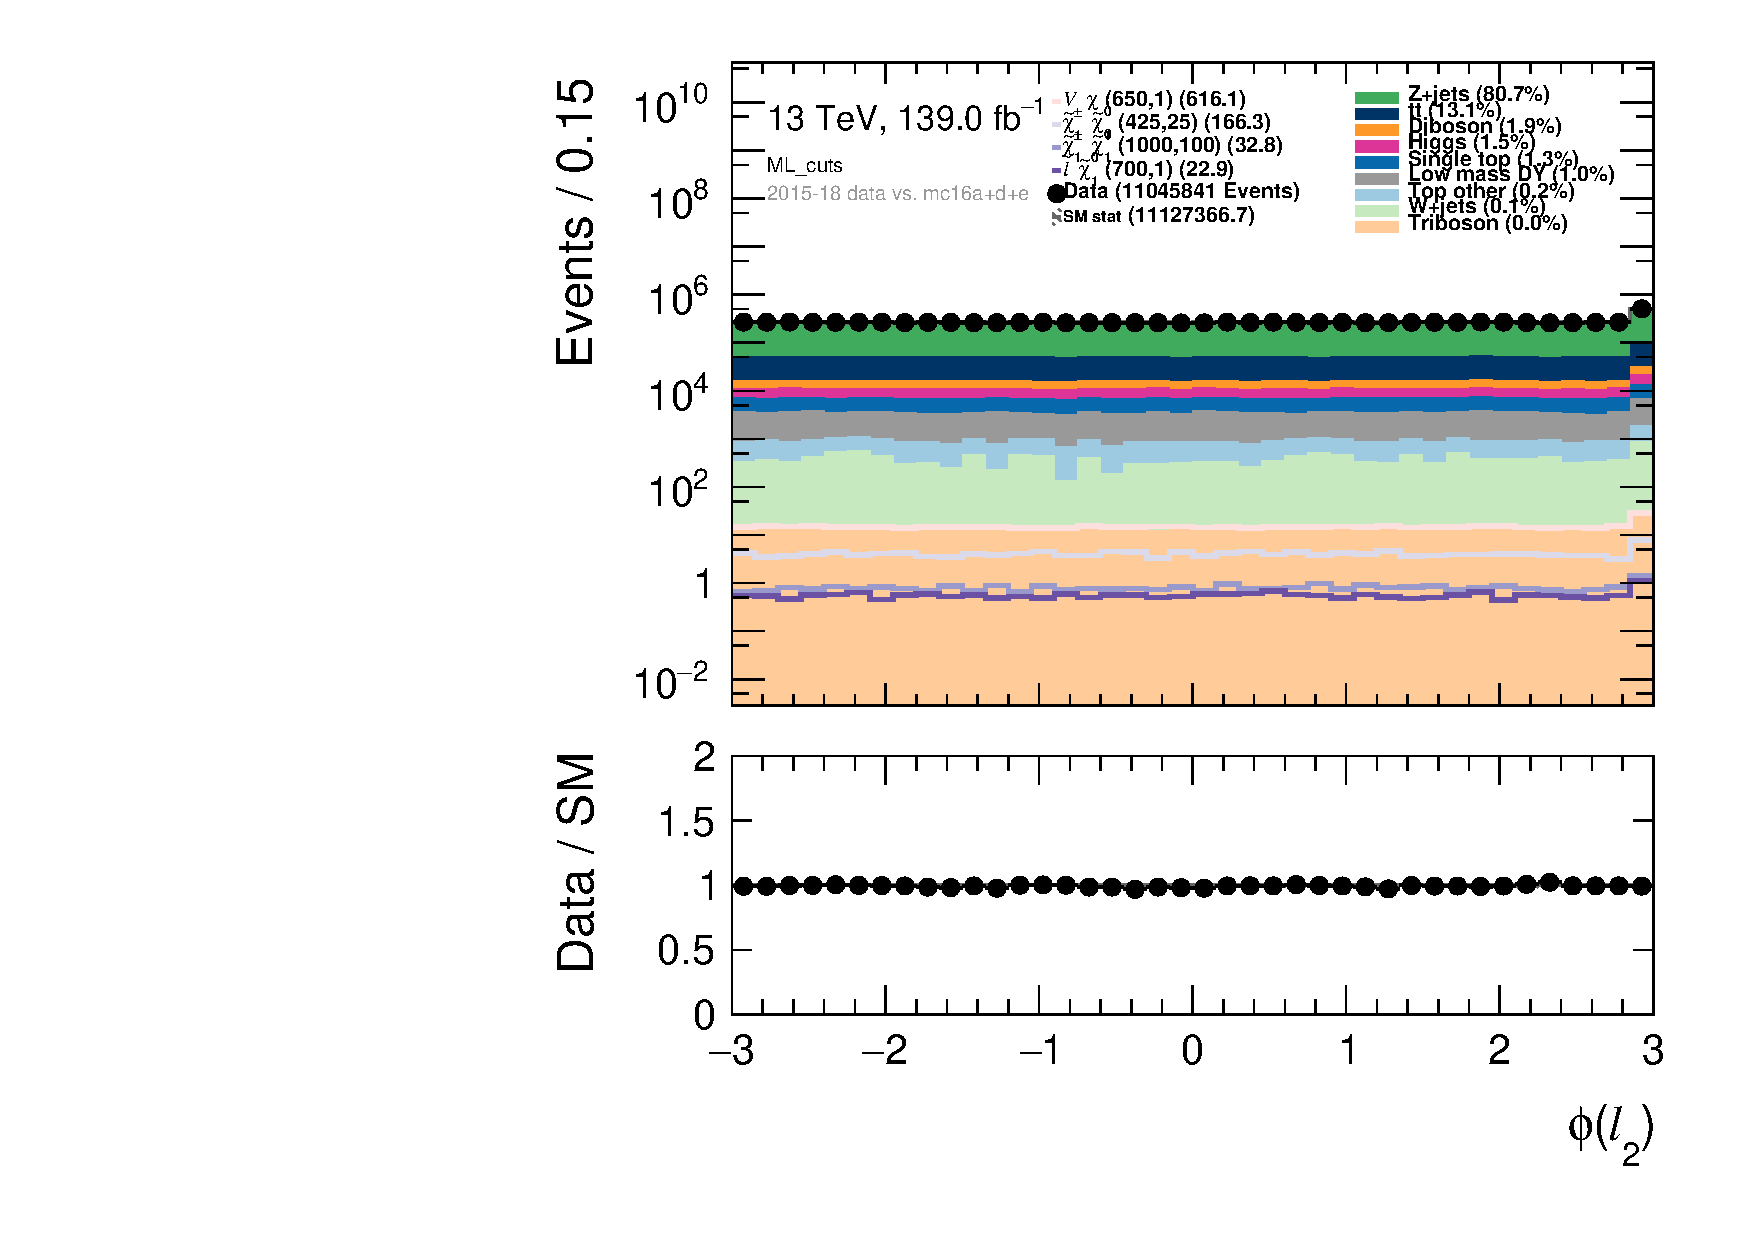
\includegraphics[width=\textwidth]{Figures/ML_cuts/hist1d_lepPhi[1]_ML_cuts.pdf}
    \caption{The azimuthal angle for lepton 2.}
    \label{fig:my_label}
    \end{subfigure}
\end{figure}

\begin{figure}[H]\ContinuedFloat
%\begin{minipage}{2\textwidth}
%\begin{adjustwidth}{-3cm}{-3cm}
\centering
    \begin{subfigure}[t!]{0.49\textwidth}
        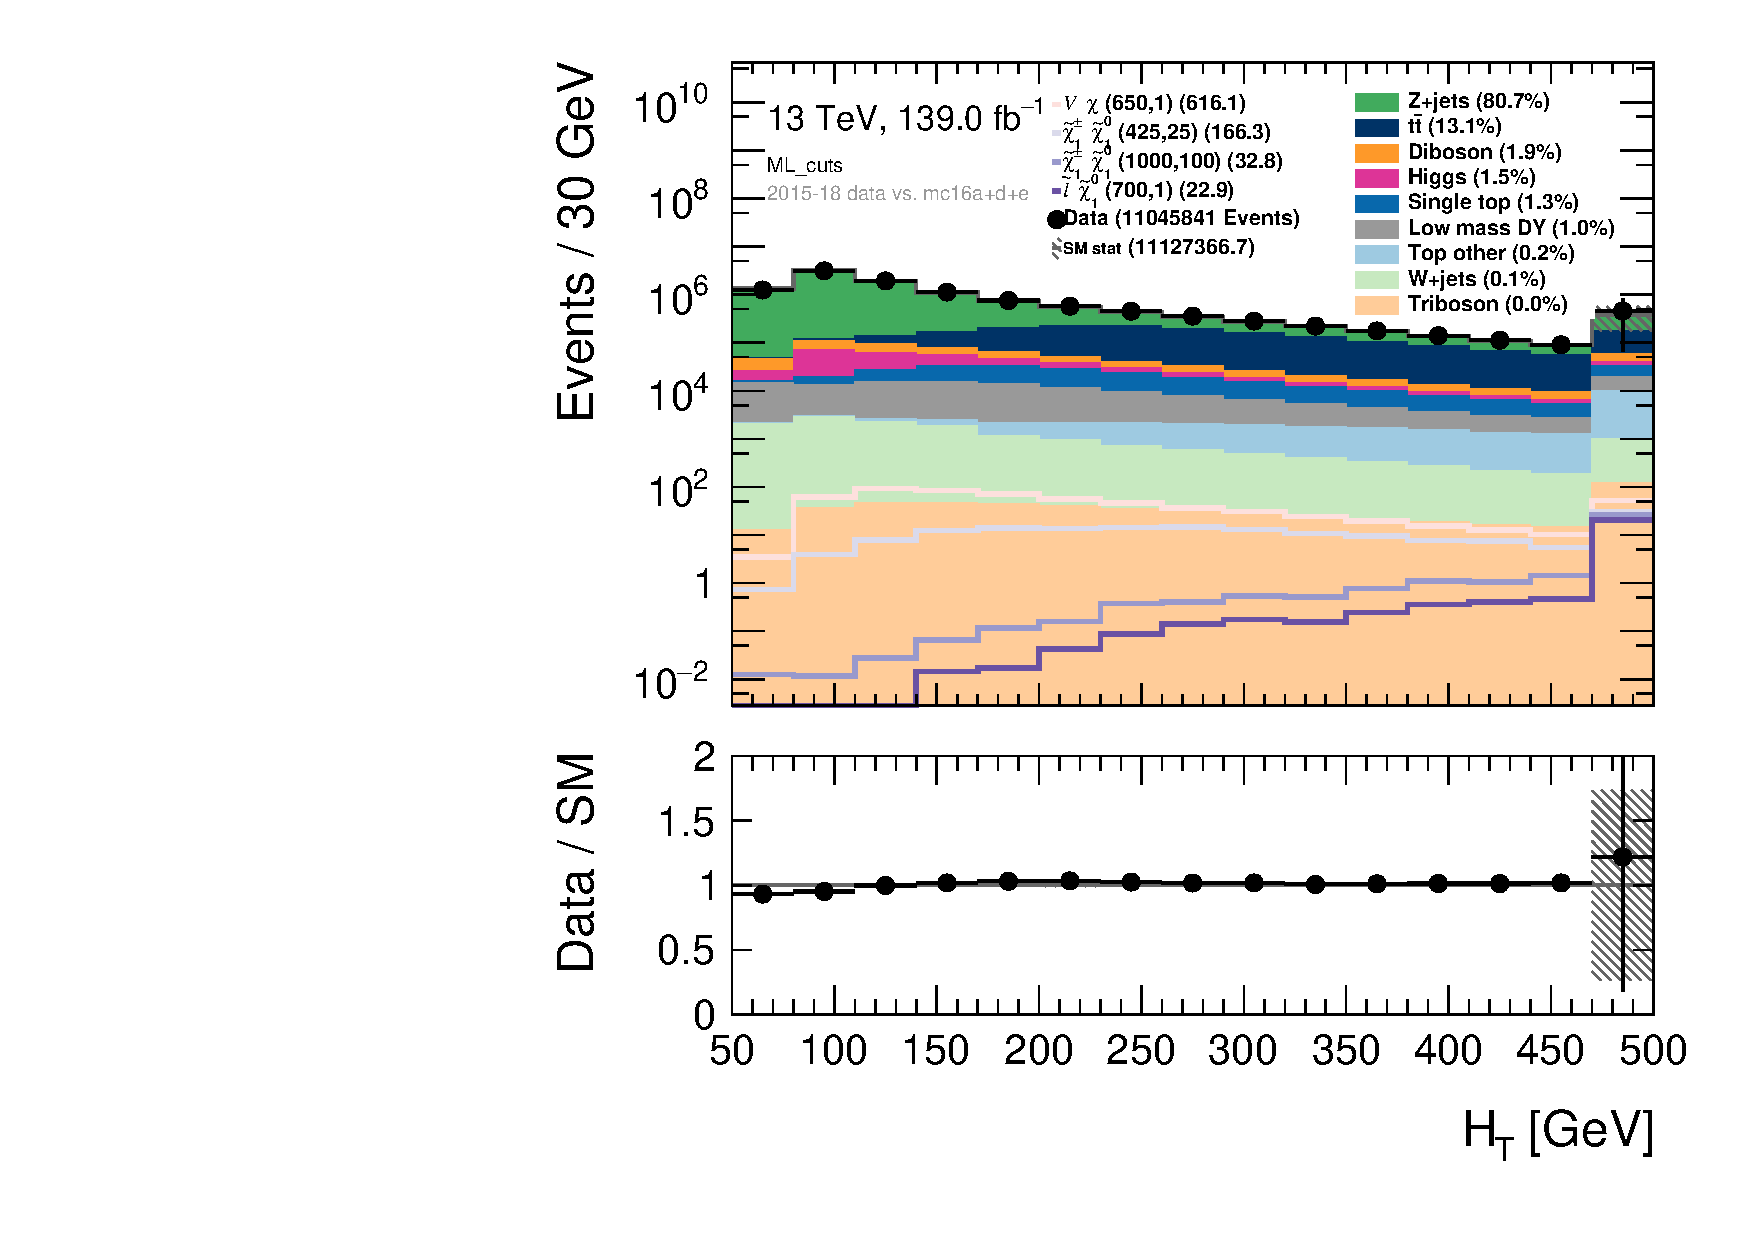
\includegraphics[width=\textwidth]{Figures/ML_cuts/hist1d_HT_ML_cuts.pdf}
    \caption{The scalar sum of the $p_T$ of the selected jets and leptons.}
    \label{fig:my_label}
    \end{subfigure}
    \begin{subfigure}[t!]{0.49\textwidth}
        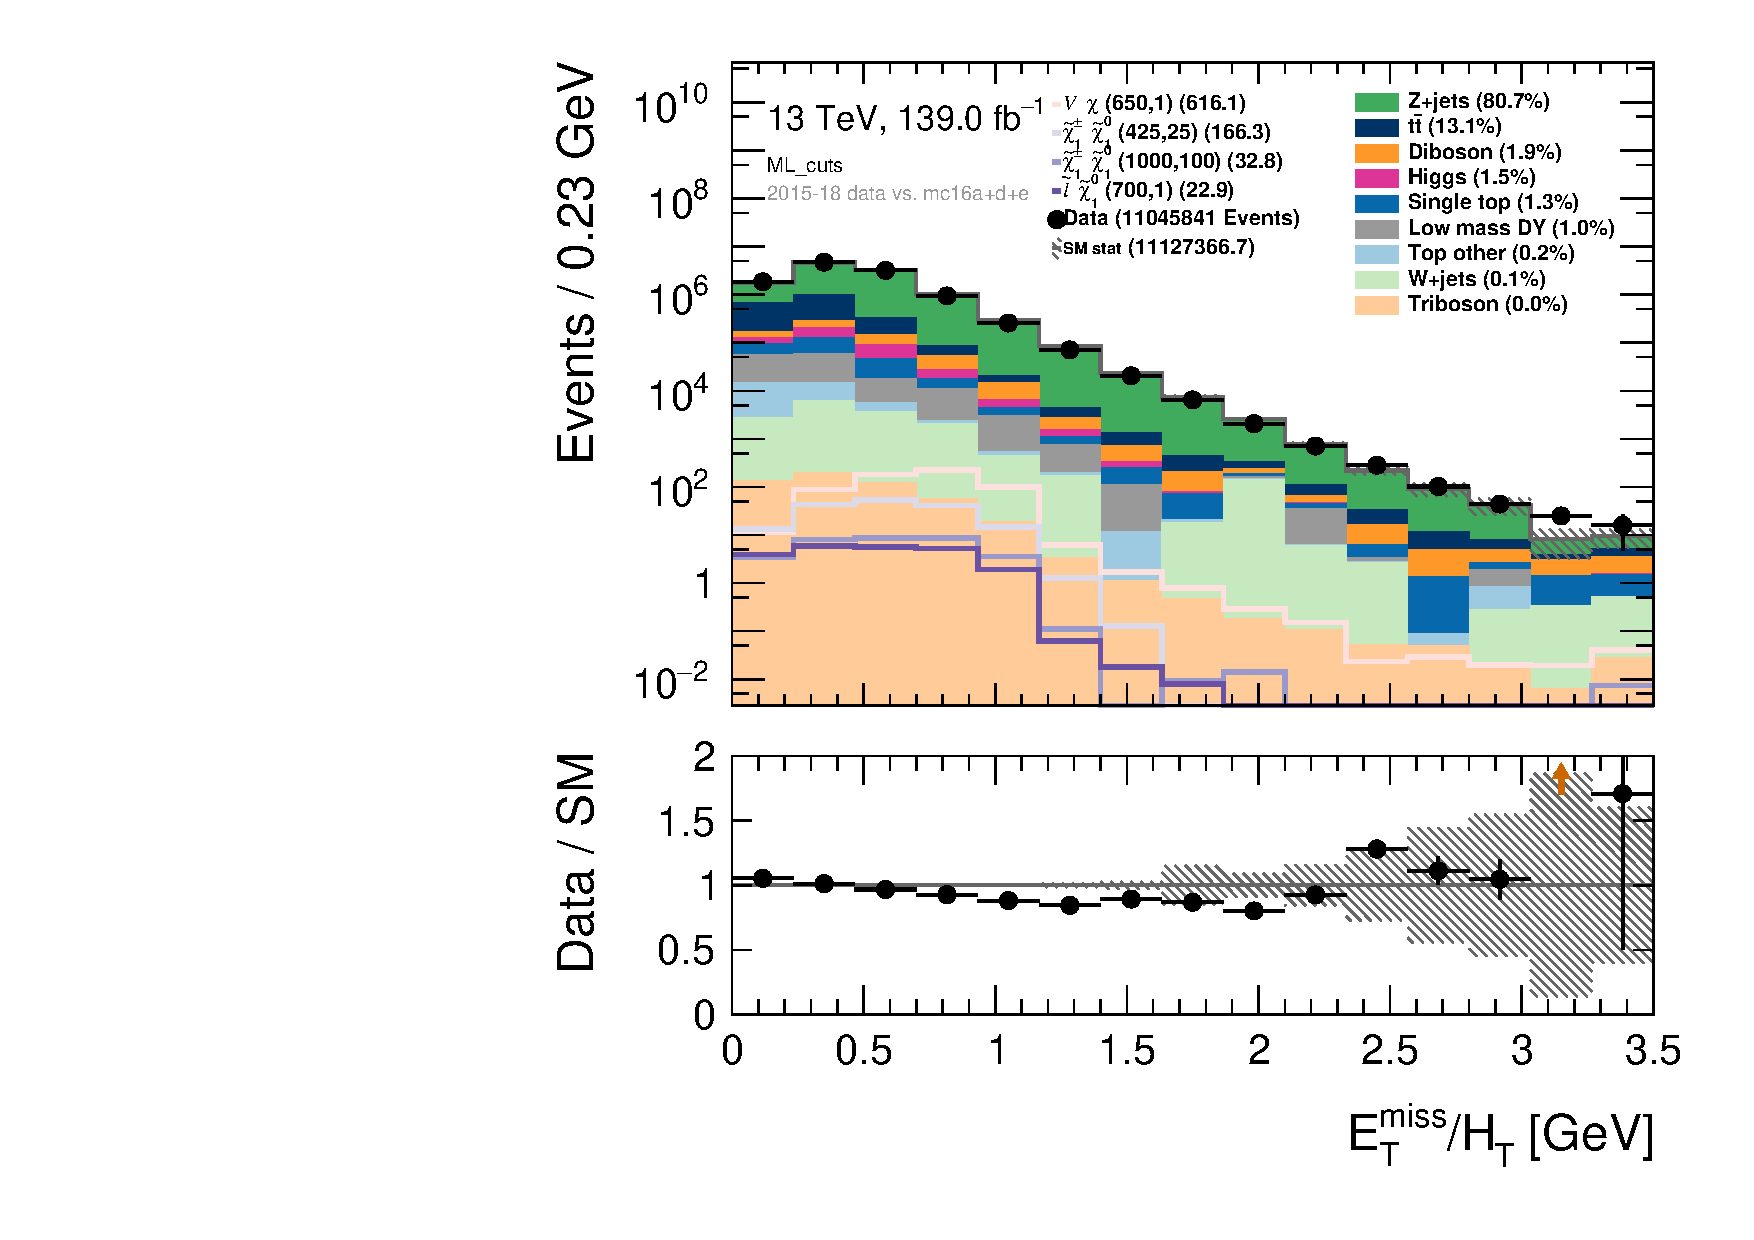
\includegraphics[width=\textwidth]{Figures/ML_cuts/hist1d_met_HT_ML_cuts.pdf}
    \caption{The ratio between $E_T^{miss}$ and $H_T$.}
    \label{fig:my_label}
    \end{subfigure}
    \begin{subfigure}[t!]{0.49\textwidth}
        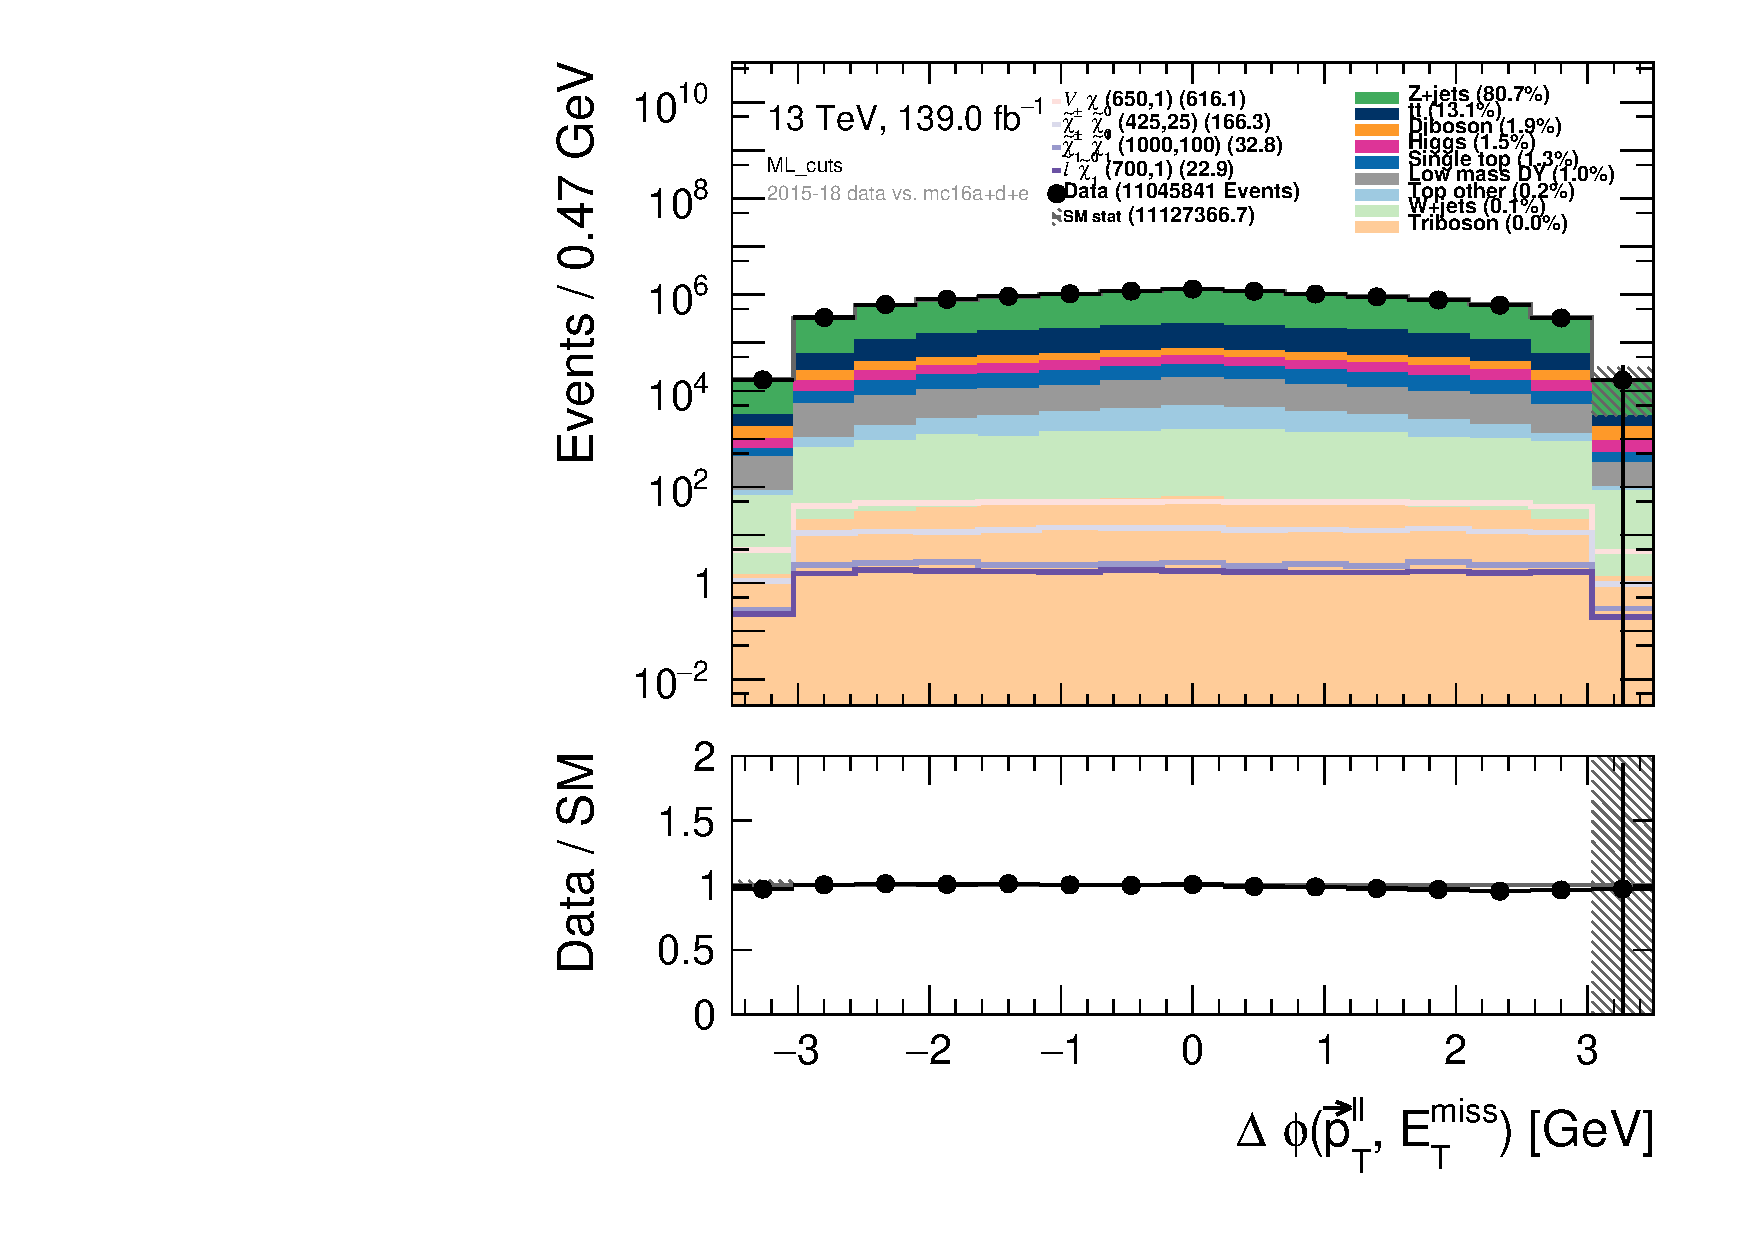
\includegraphics[width=\textwidth]{Figures/ML_cuts/hist1d_deltaPhi_ML_cuts.pdf}
    \caption{The azimuthal angle difference between the dilepton system and $E_T^{miss}$.}
    \label{fig:my_label}
    \end{subfigure}
    \begin{subfigure}[t!]{0.49\textwidth}
        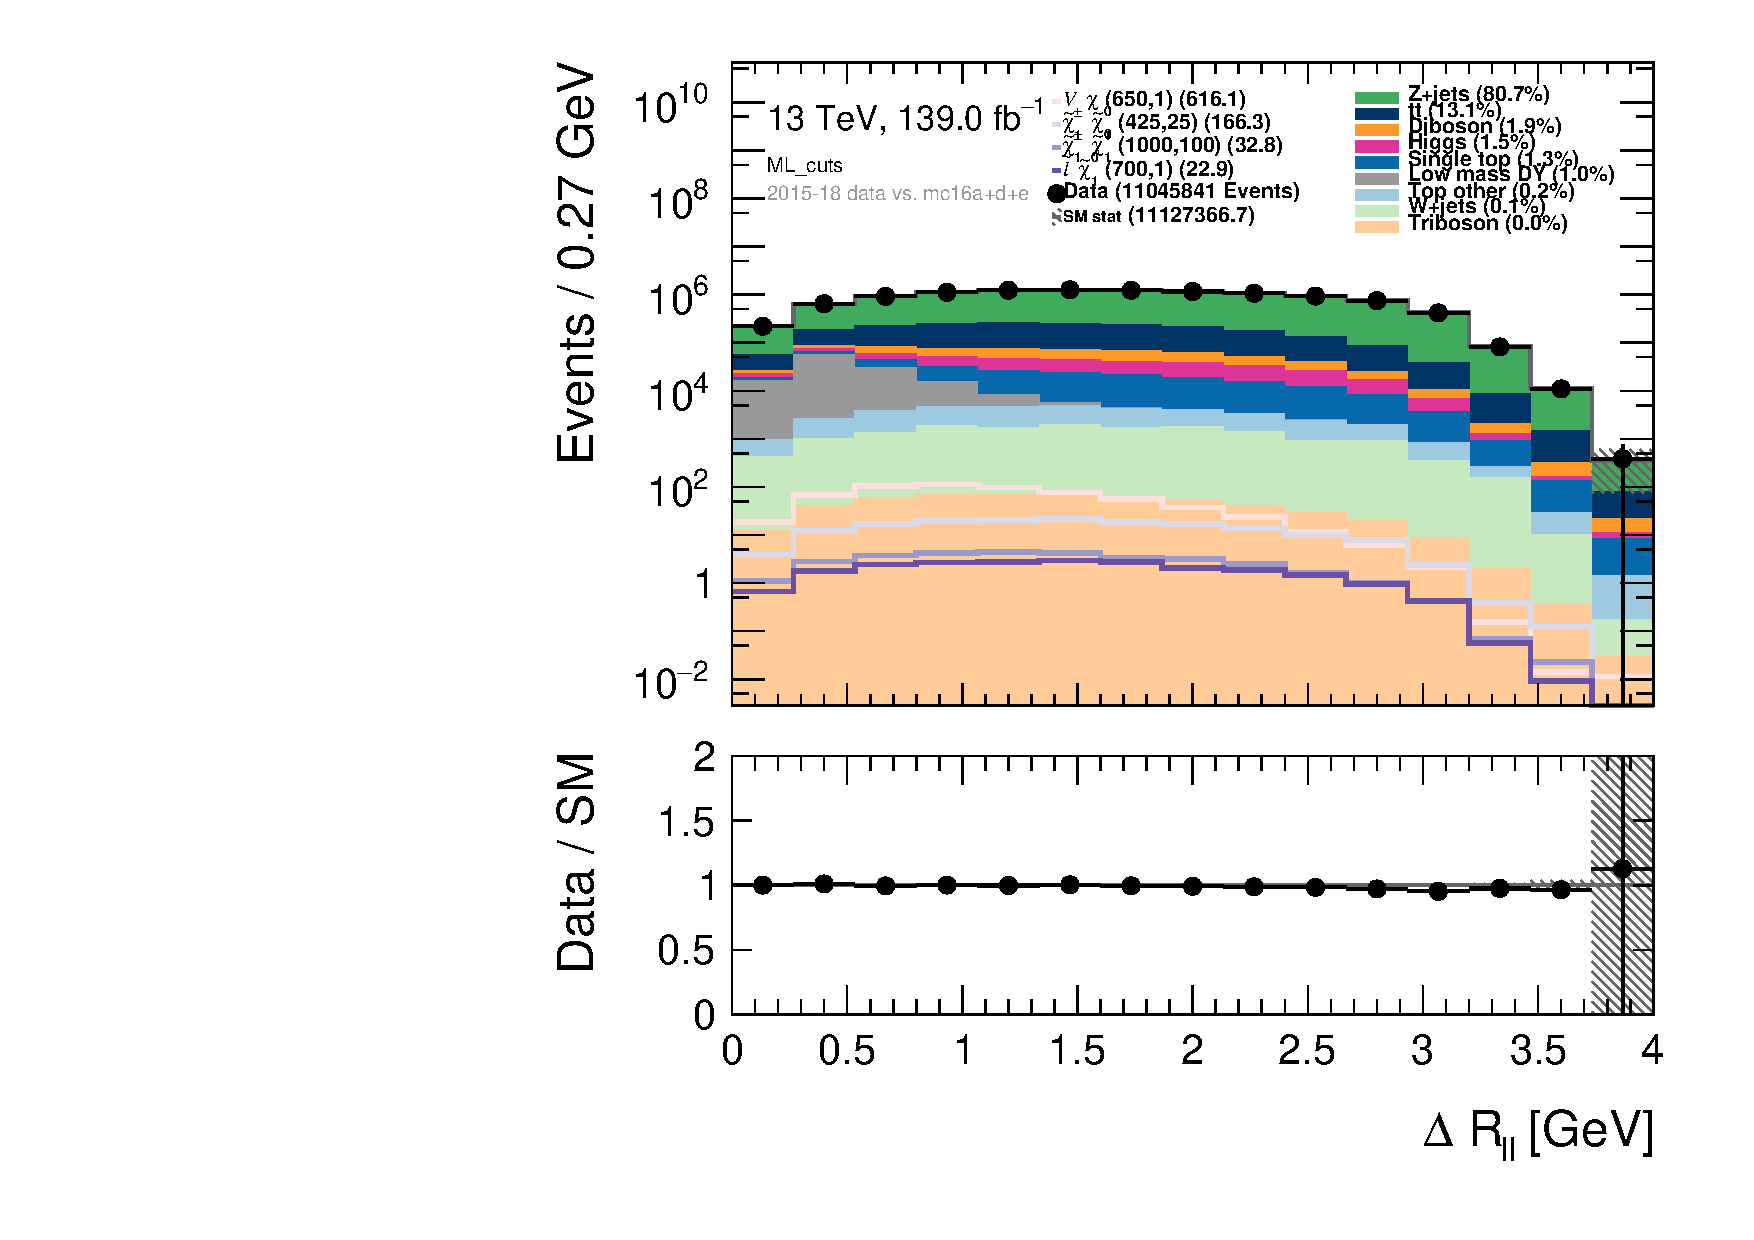
\includegraphics[width=\textwidth]{Figures/ML_cuts/hist1d_deltaRll_ML_cuts.pdf}
    \caption{Distance between the two leptons.}
    \label{fig:my_label}
    \end{subfigure}
    \begin{subfigure}[t!]{0.49\textwidth}
        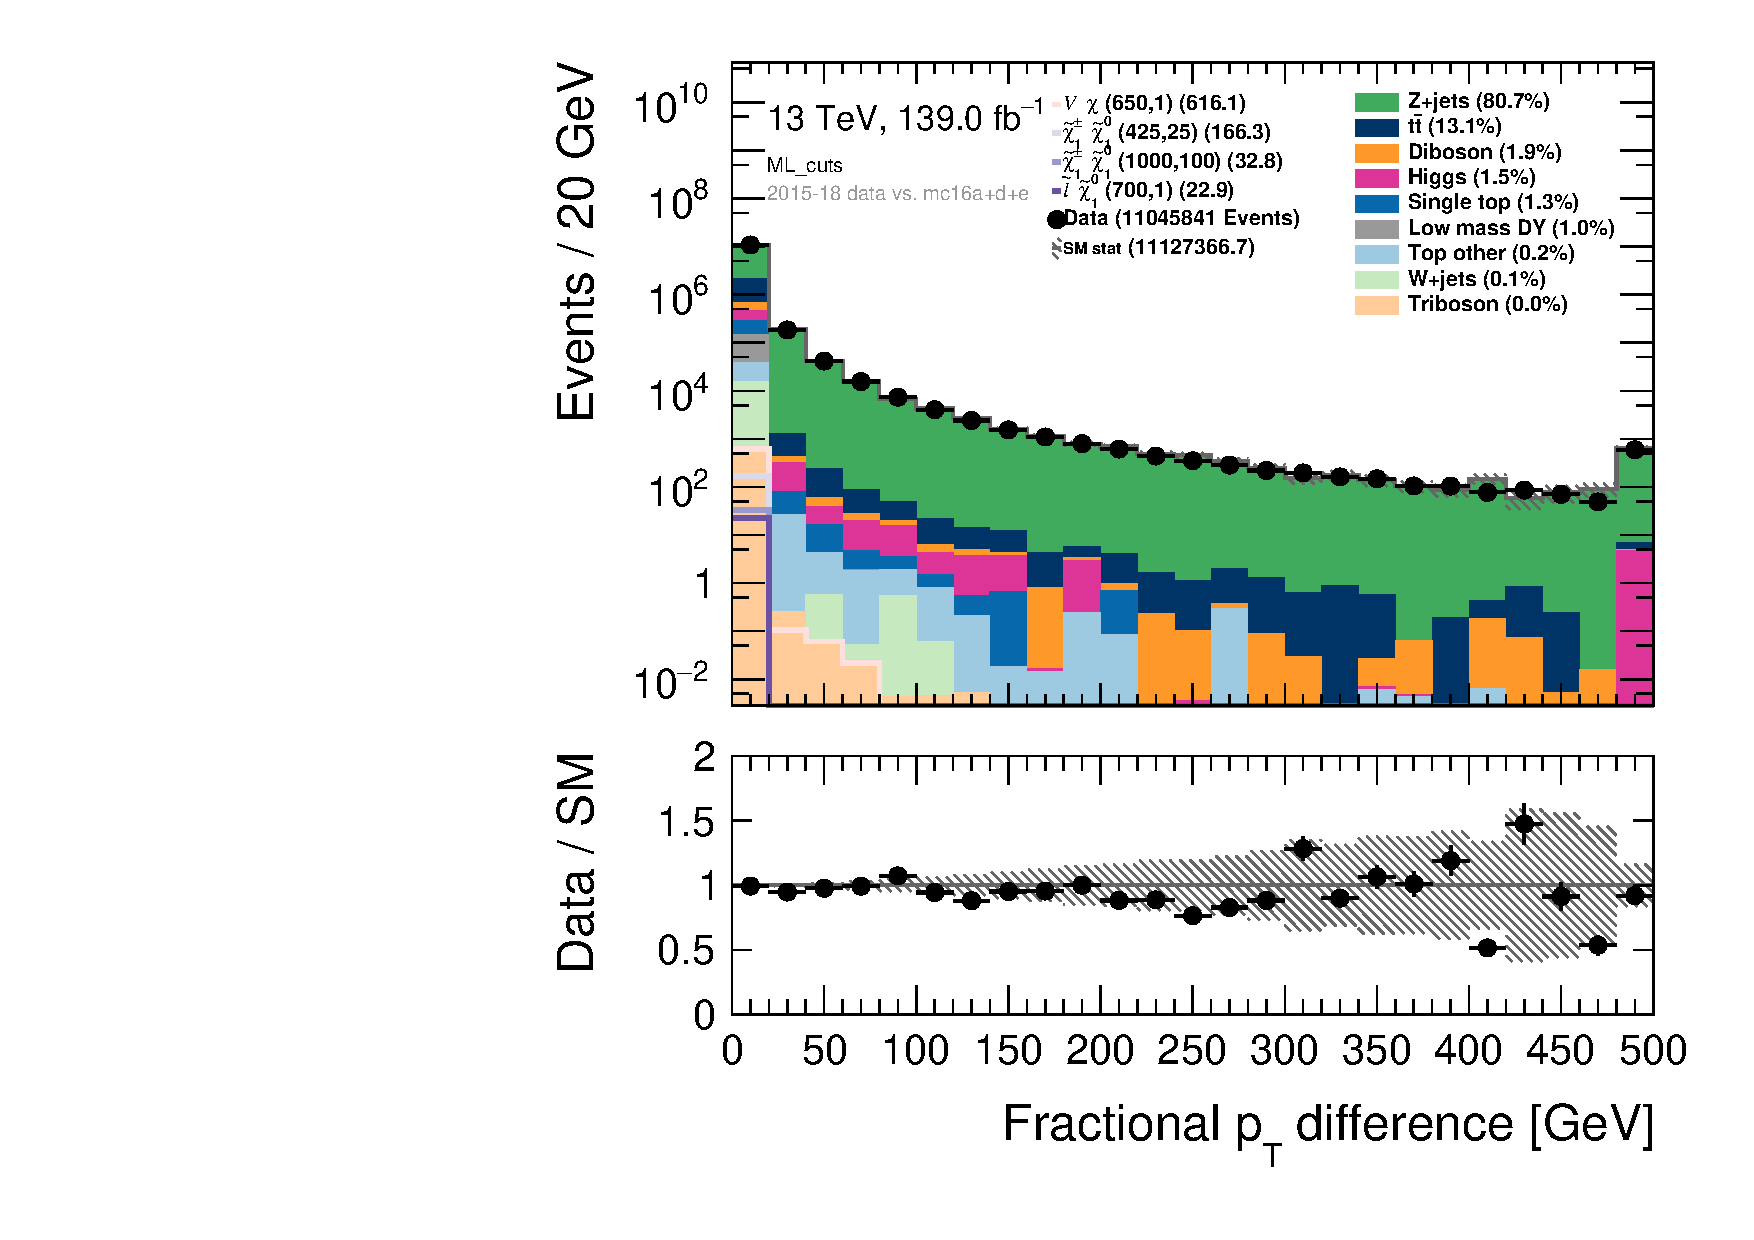
\includegraphics[width=\textwidth]{Figures/ML_cuts/hist1d_pTdiff_ML_cuts.pdf}
    \caption{The difference between the dilepton $p_T$, the selected jets $p_T$ and the vector sum of $\Vec{E}_T^{miss}$.}
    \label{fig:my_label}
    \end{subfigure}
    \begin{subfigure}[t!]{0.49\textwidth}
        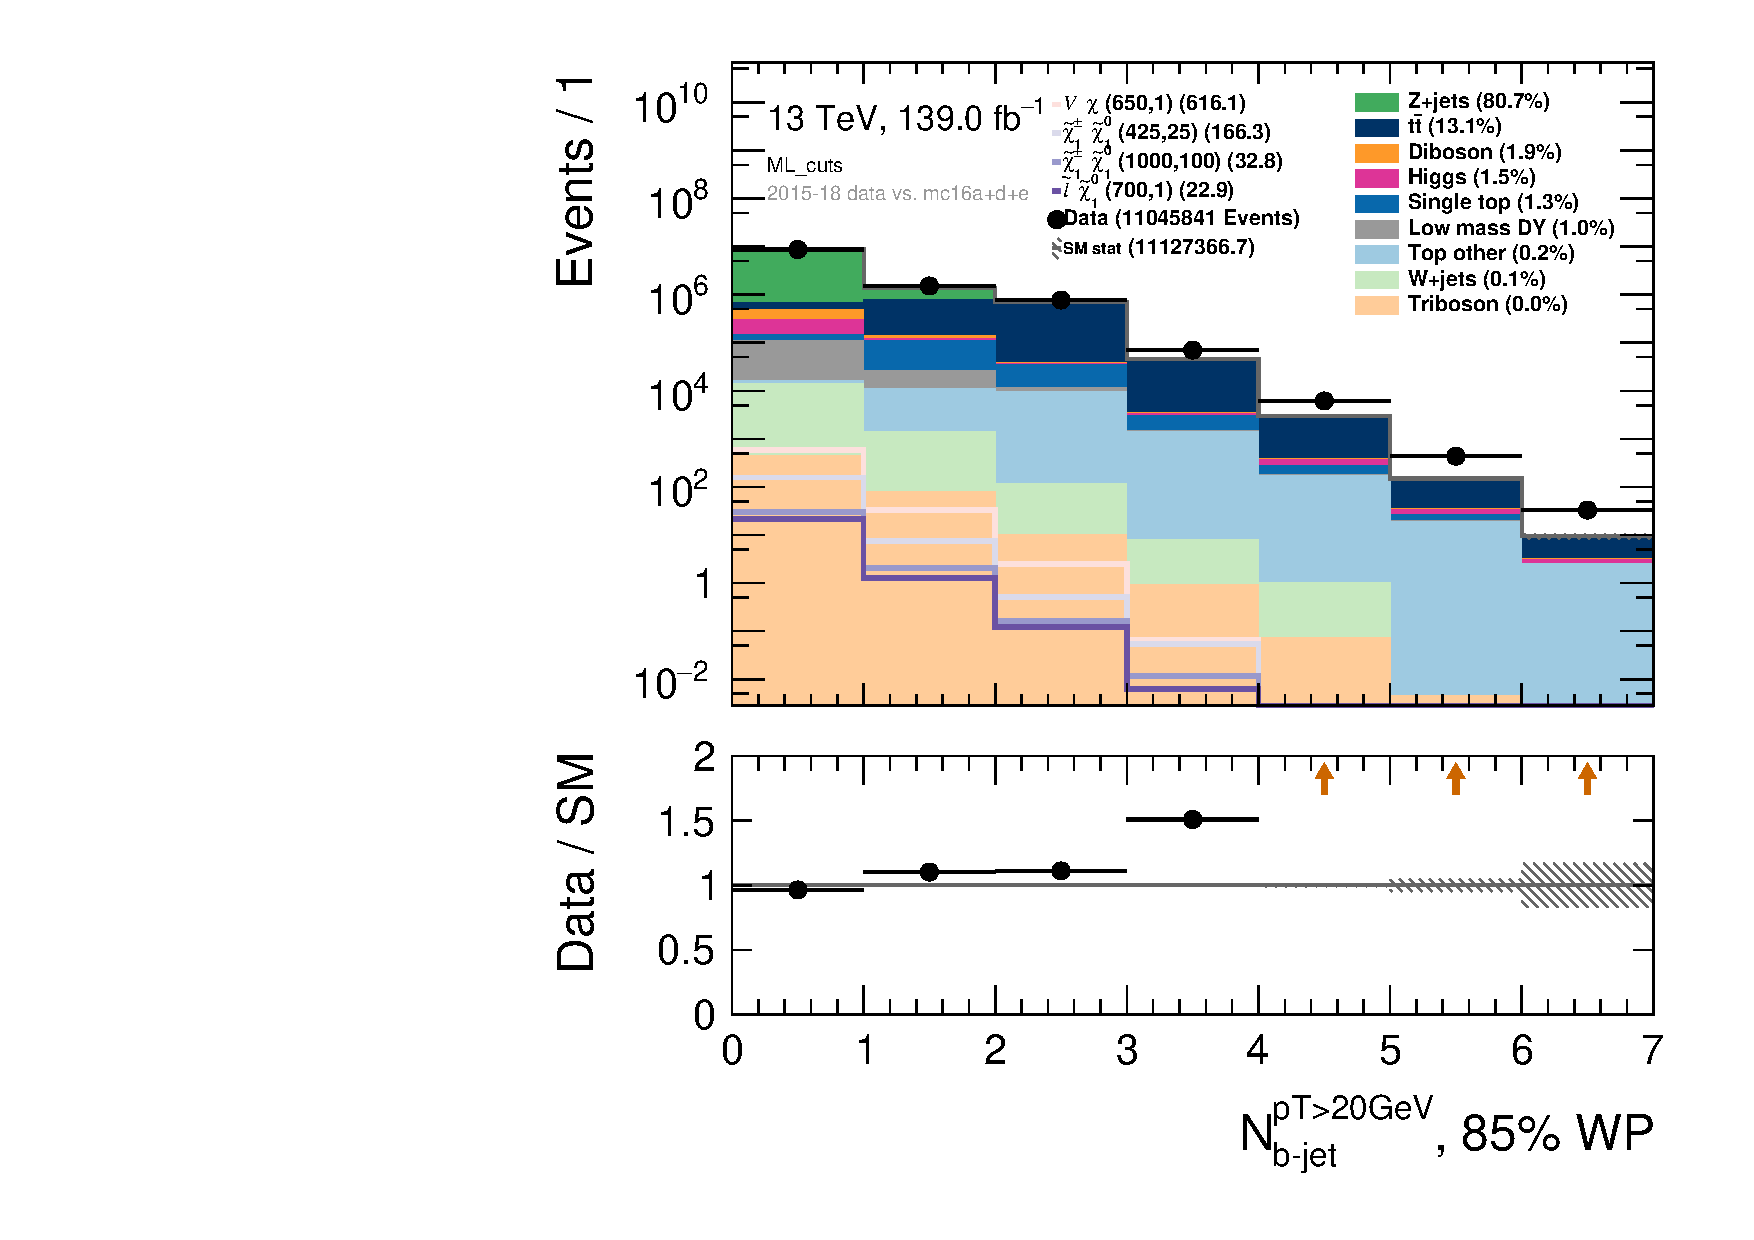
\includegraphics[width=\textwidth]{Figures/ML_cuts/hist1d_nBJet20_MV2c10_FixedCutBEff_85_ML_cuts.pdf}
    \caption{B-jets.}
    \label{fig:bjetMLcuts}
    \end{subfigure}
\end{figure}

\begin{figure}[H]\ContinuedFloat
%\begin{minipage}{2\textwidth}
%\begin{adjustwidth}{-3cm}{-3cm}
\centering
%\advance\leftskip-4cm 
%\advance\rightskip-4cm 
    \begin{subfigure}[t!]{0.49\textwidth}
        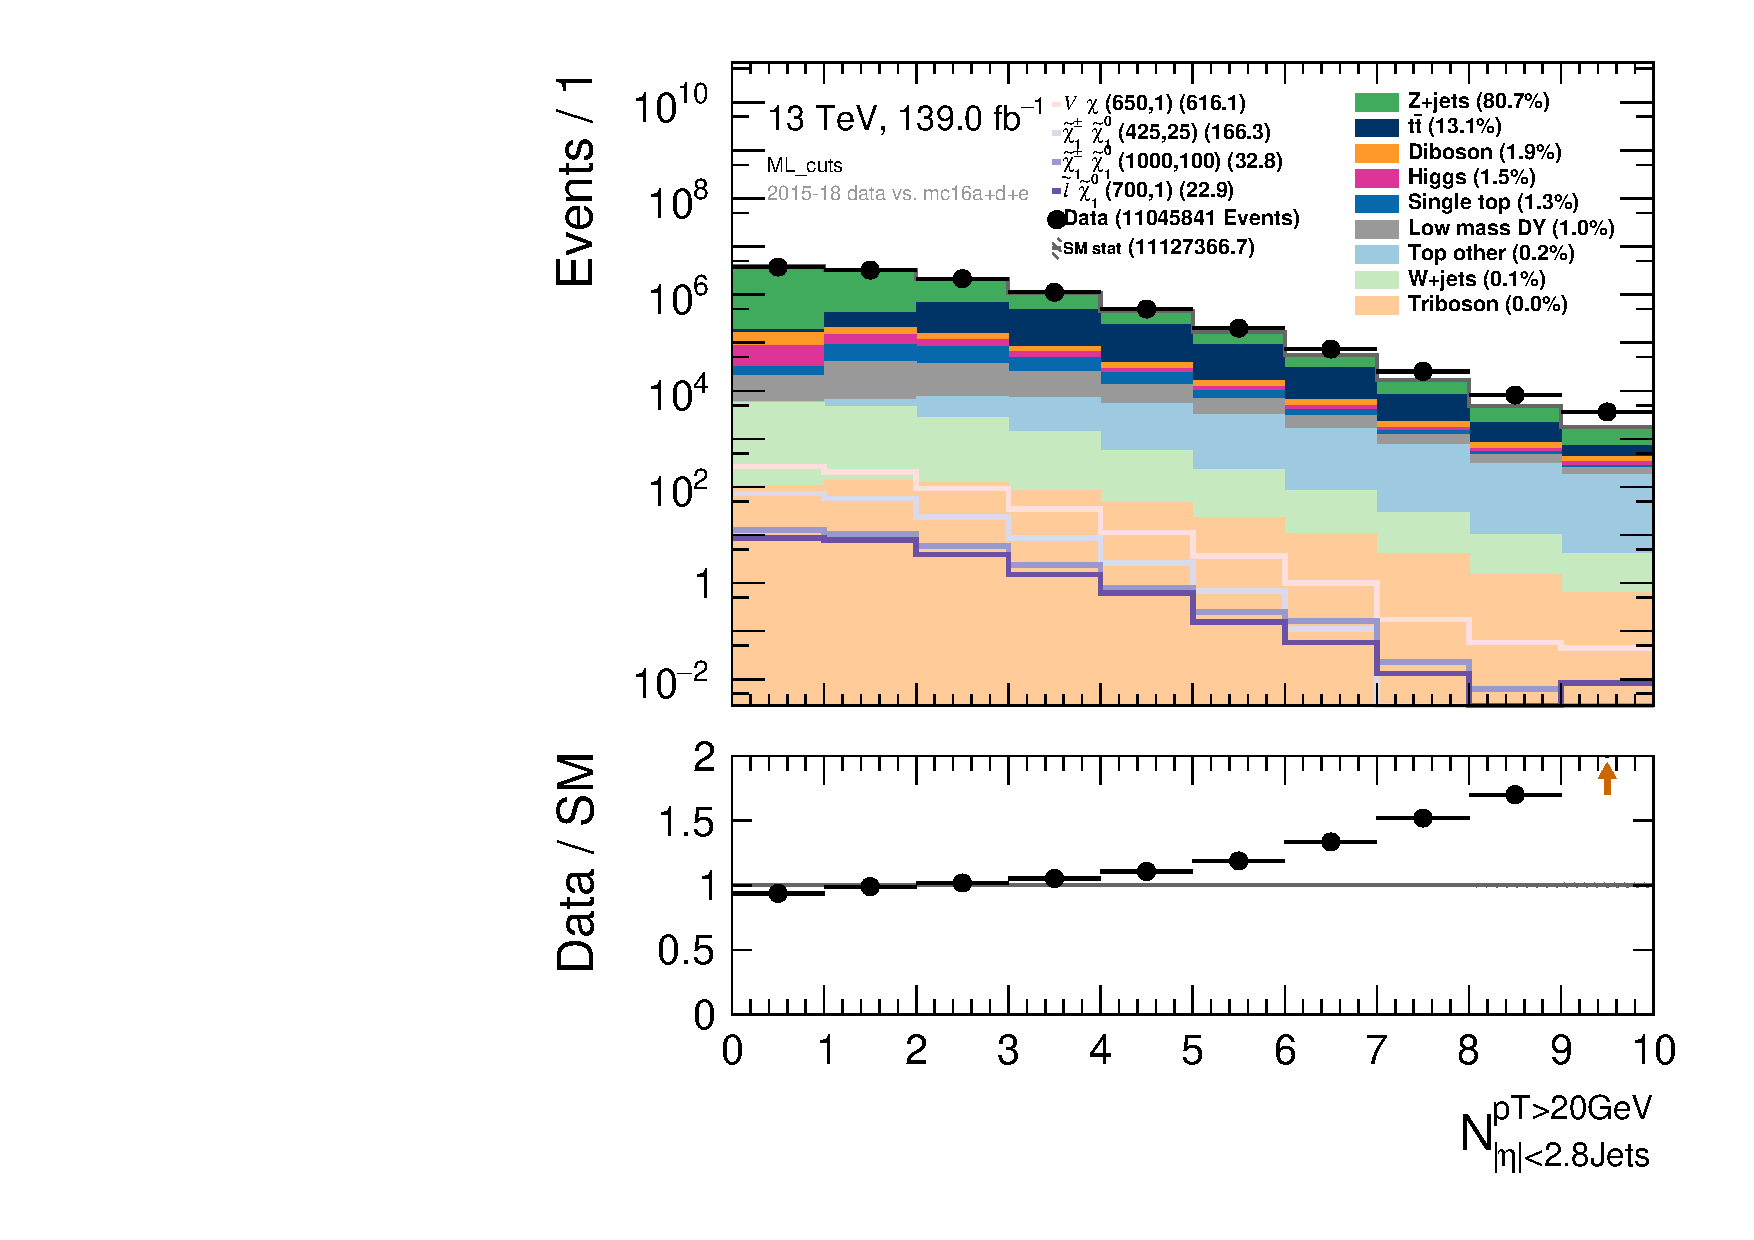
\includegraphics[width=\textwidth]{Figures/ML_cuts/hist1d_nJet20_ML_cuts.pdf}
    \caption{Jets with $p_T > 20$ GeV.}
    \label{fig:my_label}
    \end{subfigure}
    \begin{subfigure}[t!]{0.49\textwidth}
        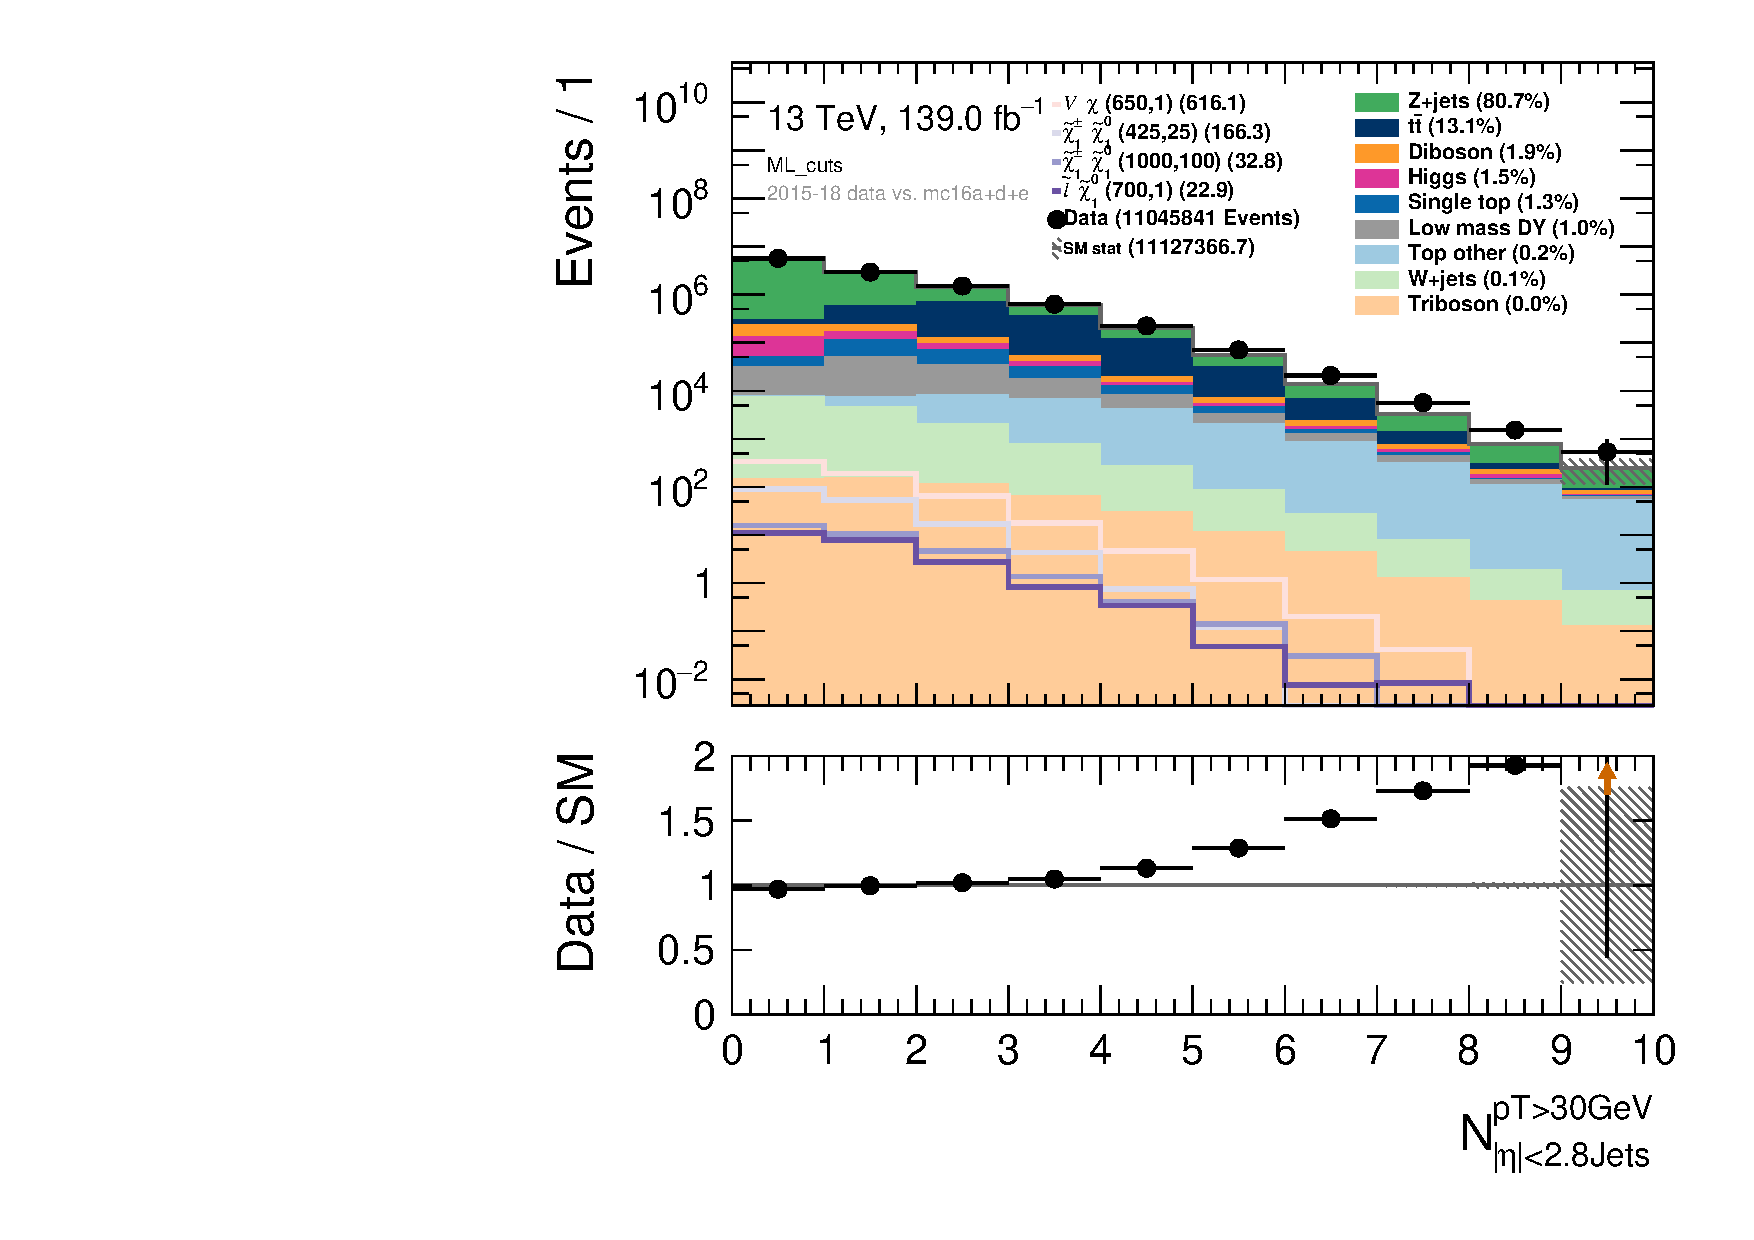
\includegraphics[width=\textwidth]{Figures/ML_cuts/hist1d_nJet30_ML_cuts.pdf}
   \caption{Jets with $p_T > 30$ GeV.}
   \label{fig:my_label}
    \end{subfigure}
    \\
    \begin{subfigure}[t!]{0.49\textwidth}
        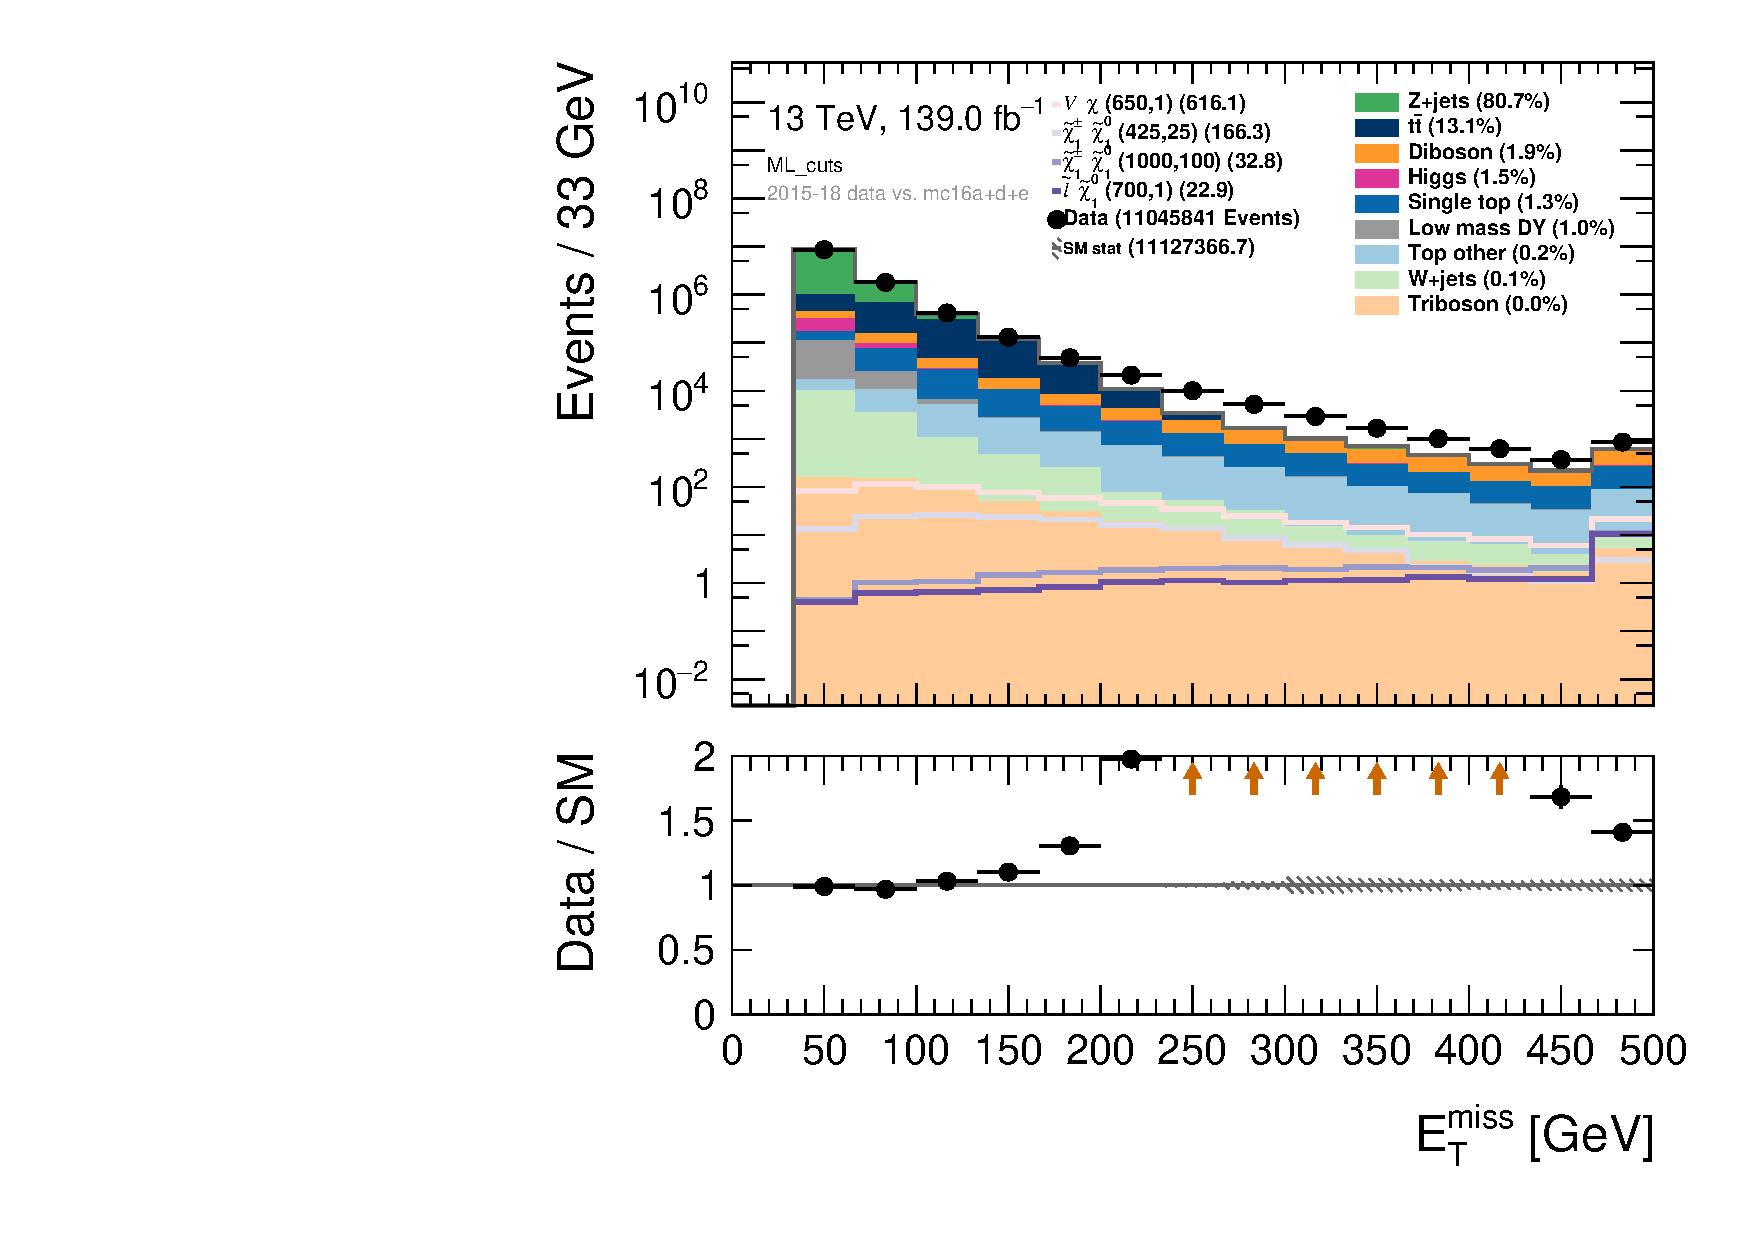
\includegraphics[width=\textwidth]{Figures/ML_cuts/hist1d_met_Et_ML_cuts.pdf}
    \caption{Missing transverse energy.}
    \label{fig:metMLcuts}
    \end{subfigure}
    \begin{subfigure}[t!]{0.49\textwidth}
        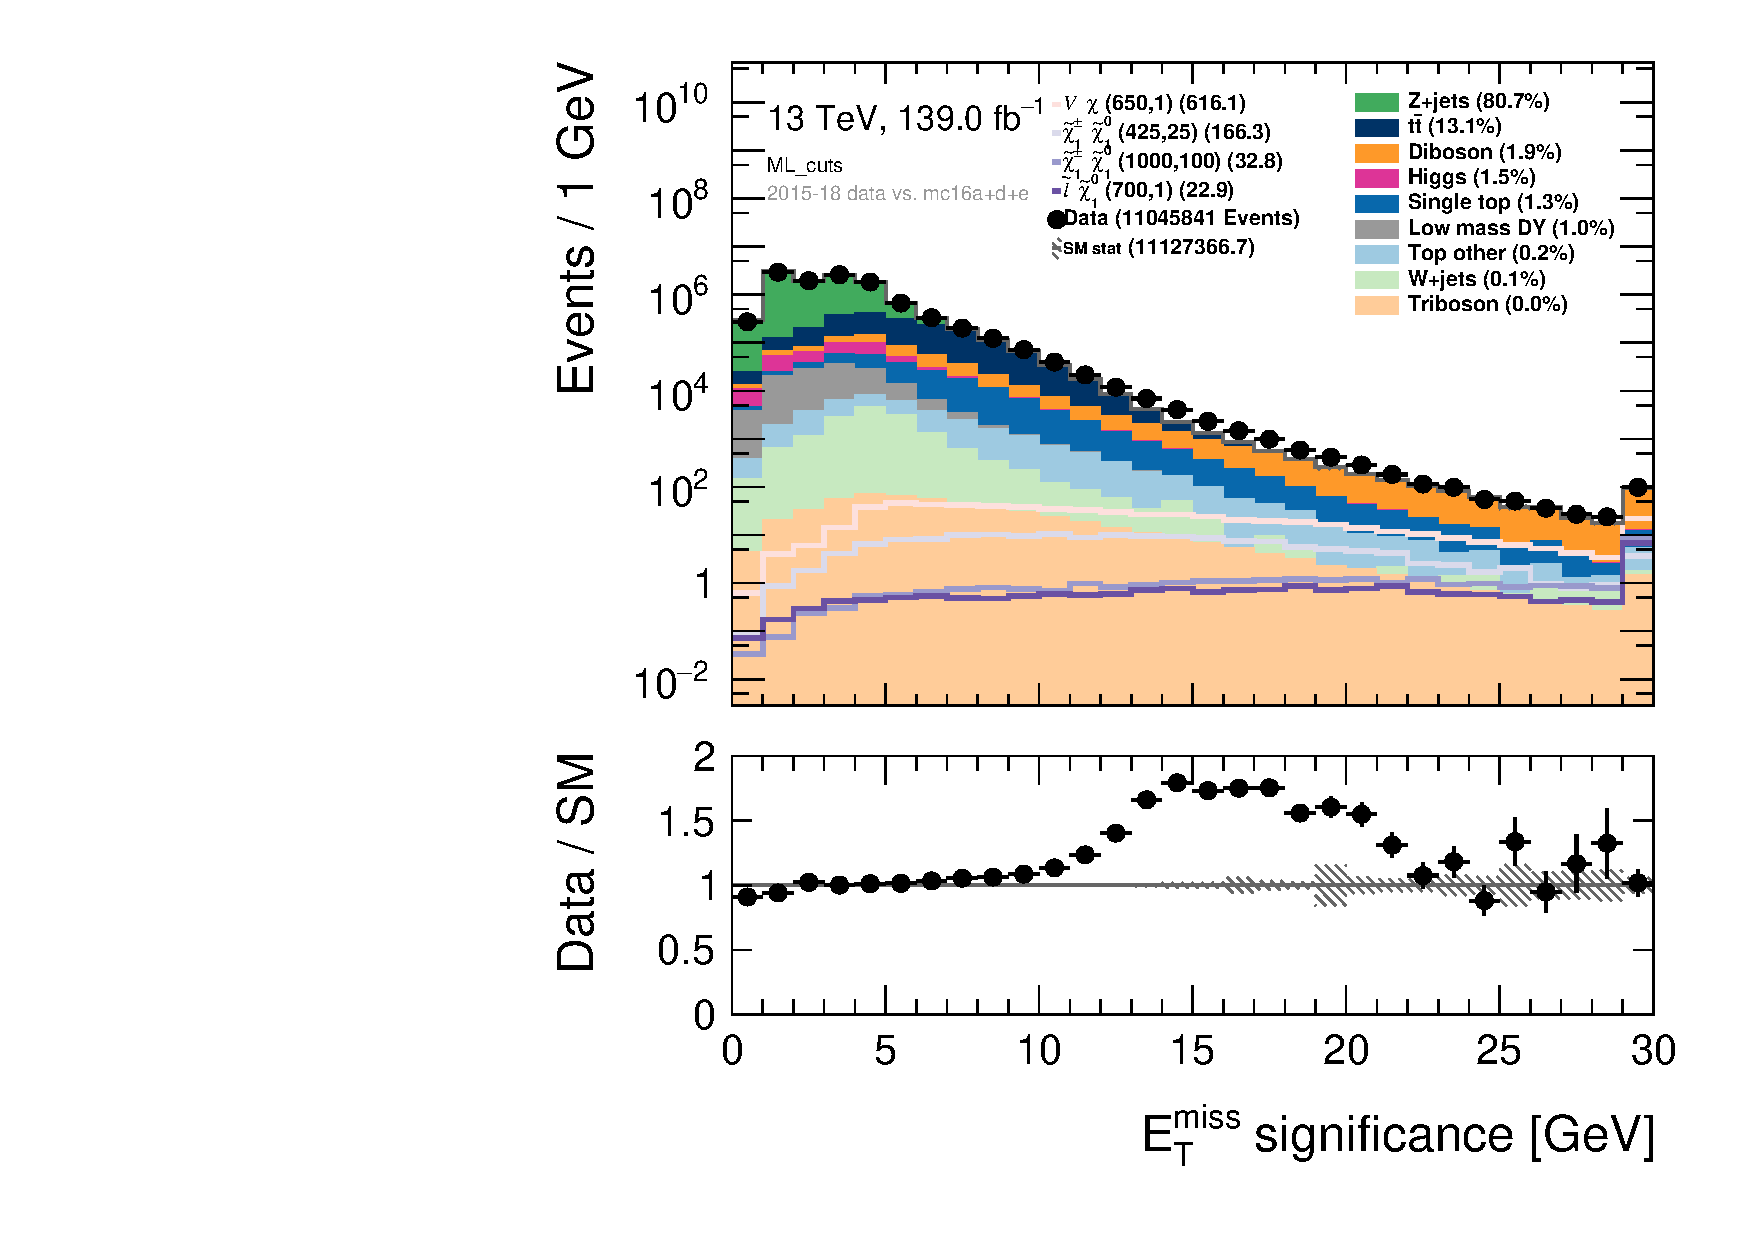
\includegraphics[width=\textwidth]{Figures/ML_cuts/hist1d_met_Sign_ML_cuts.pdf}
    \caption{Missing transverse energy significance.}
    \label{fig:metSignMLcuts}
    \end{subfigure}
    \\
    \begin{subfigure}[t!]{0.49\textwidth}
        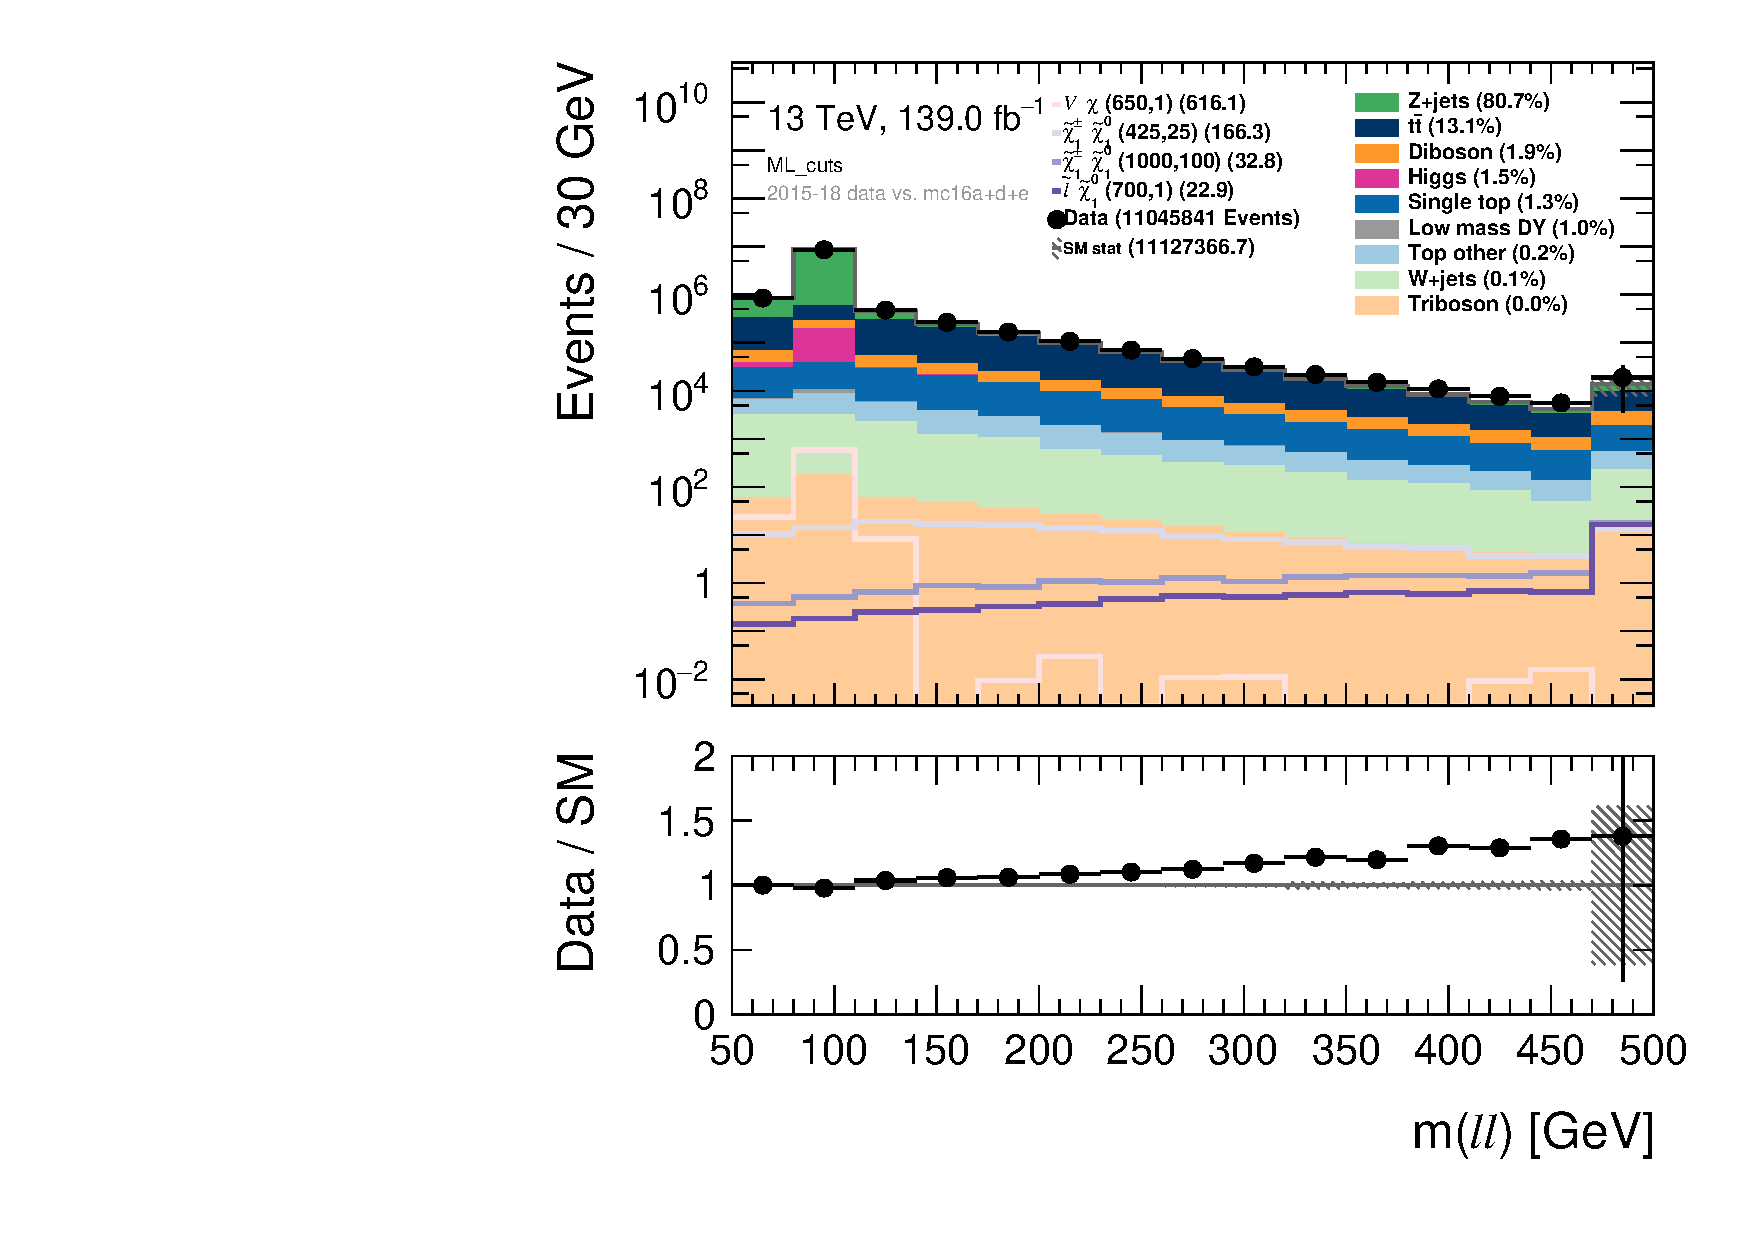
\includegraphics[width=\textwidth]{Figures/ML_cuts/hist1d_mll_ML_cuts.pdf}
    \caption{Invariant mass.}
    \label{fig:my_label}
    \end{subfigure}
    \begin{subfigure}[t!]{0.49\textwidth}
        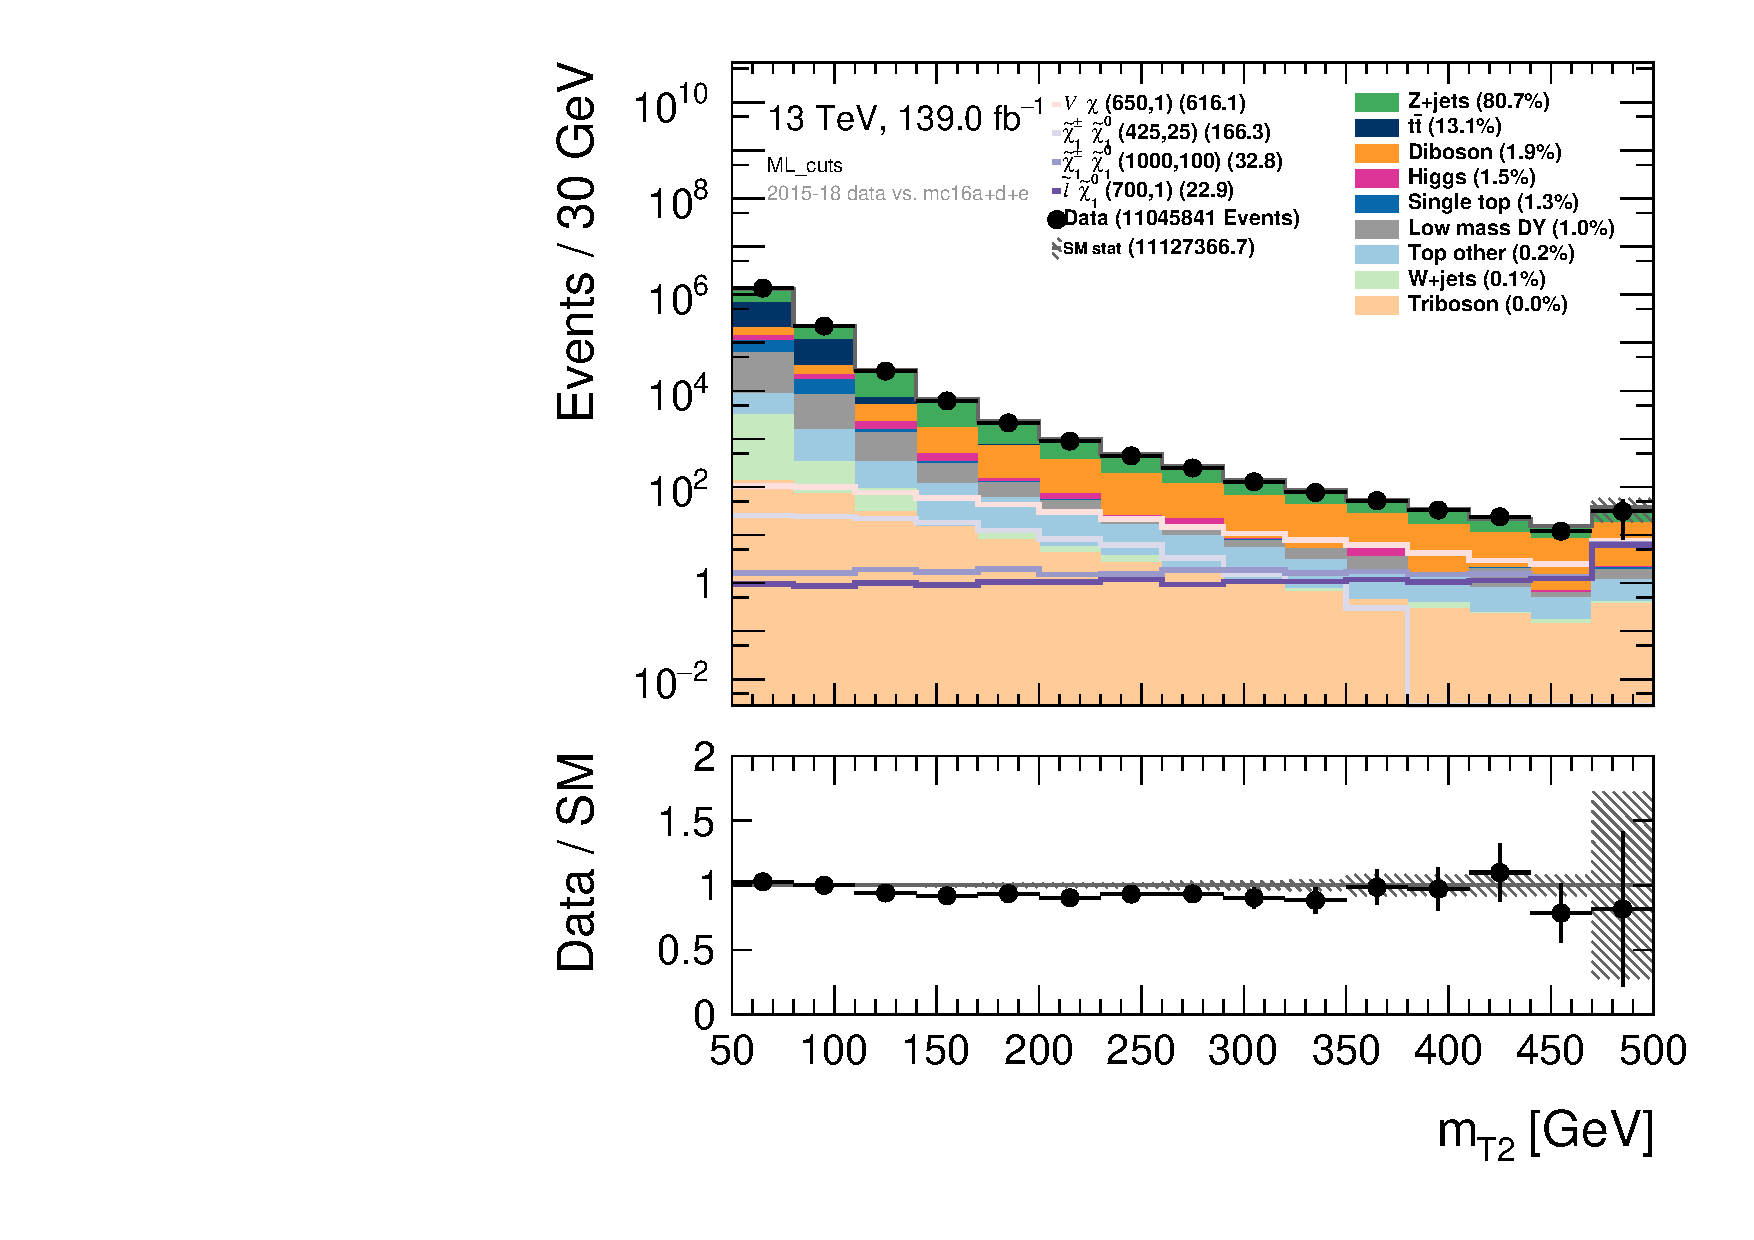
\includegraphics[width=\textwidth]{Figures/ML_cuts/hist1d_mt2_ML_cuts.pdf}
    \caption{Stransverse mass.}
    \label{fig:my_label}
    \end{subfigure}
\end{figure}

\begin{figure}[H]\ContinuedFloat
%\begin{minipage}{2\textwidth}
%\begin{adjustwidth}{-3cm}{-3cm}
\centering
    \begin{subfigure}[t!]{0.49\textwidth}
        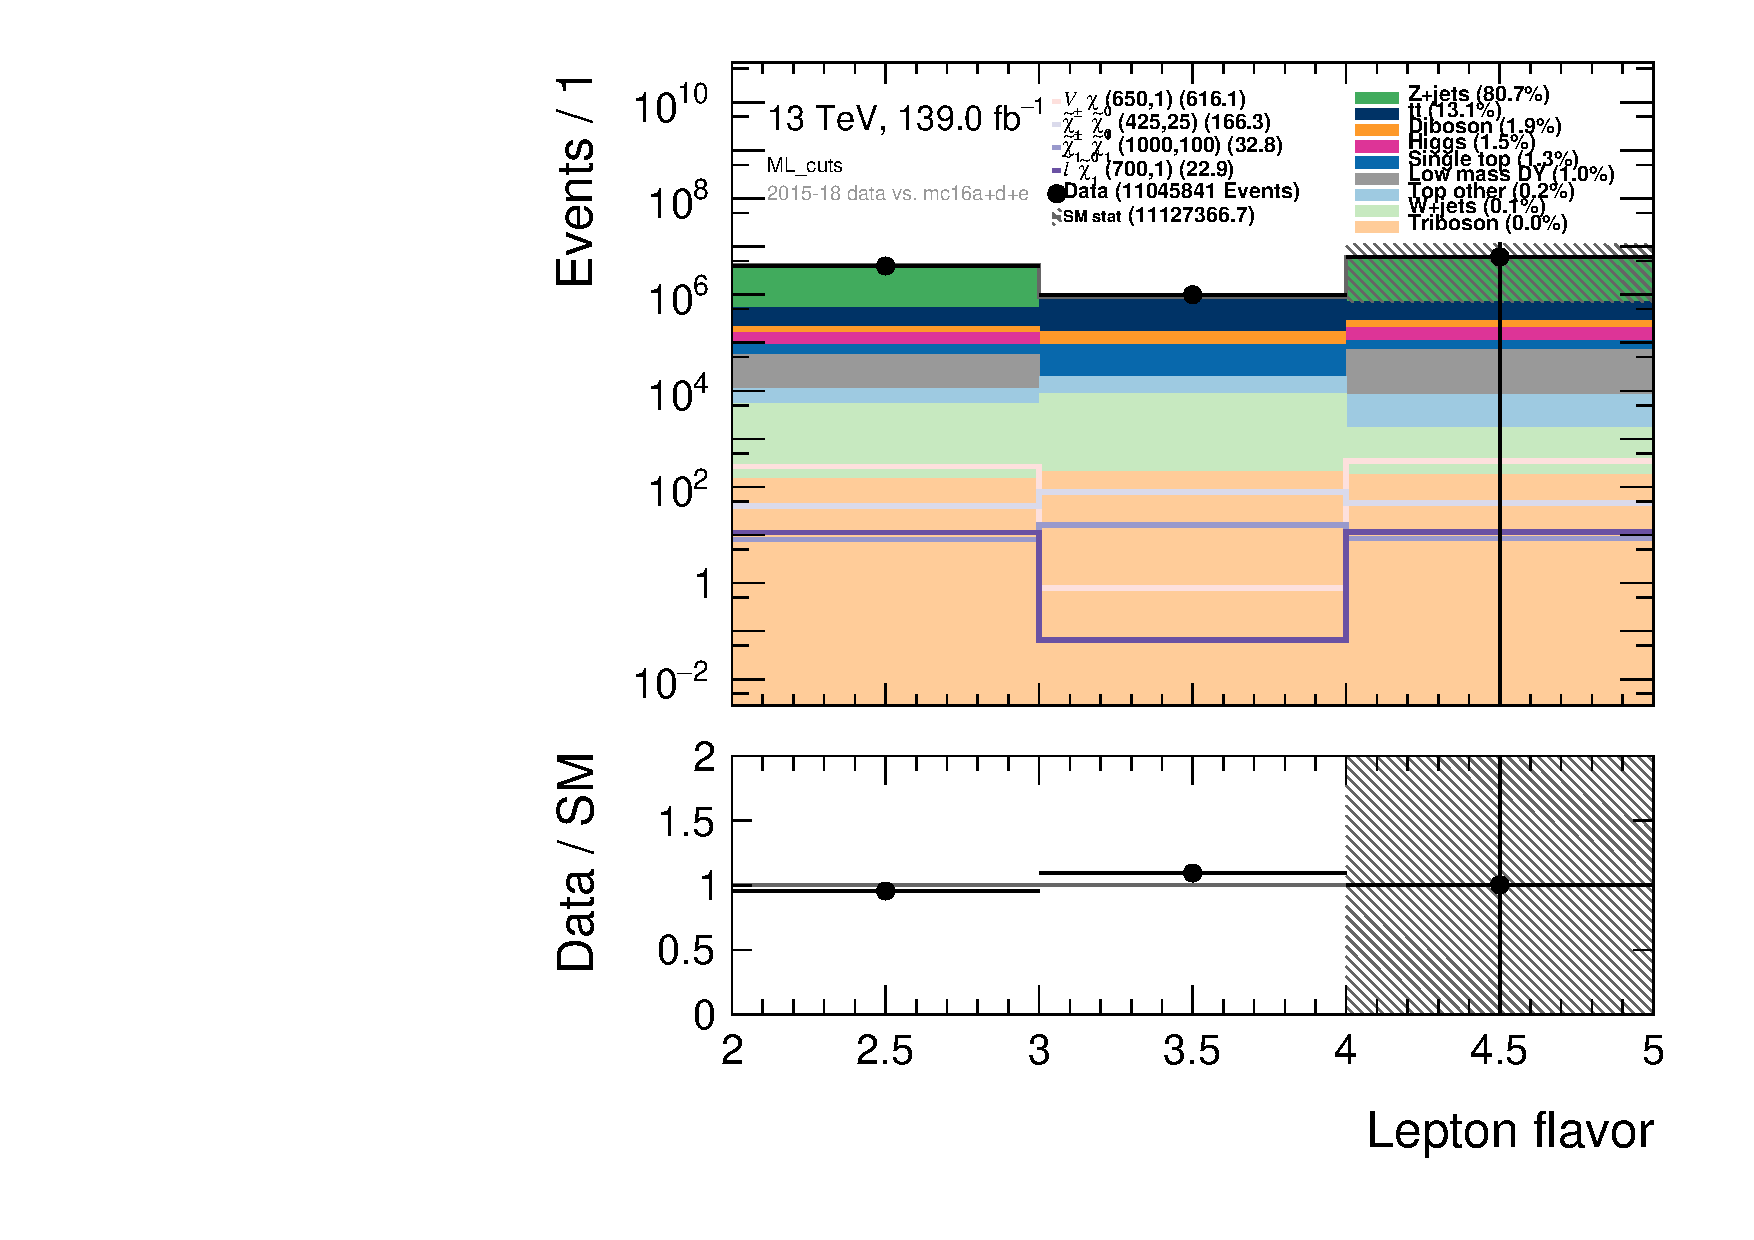
\includegraphics[width=\textwidth]{Figures/ML_cuts/hist1d_lepFlavor[0]+lepFlavor[1]_ML_cuts.pdf}
    \caption{Flavor combinations of the two leptons, with the first, second and third bin corresponding to $ee$, $e\mu$ and $\mu\mu$ events, respectively.}
    \label{fig:my_label}
    \end{subfigure}
    \begin{subfigure}[t!]{0.49\textwidth}
        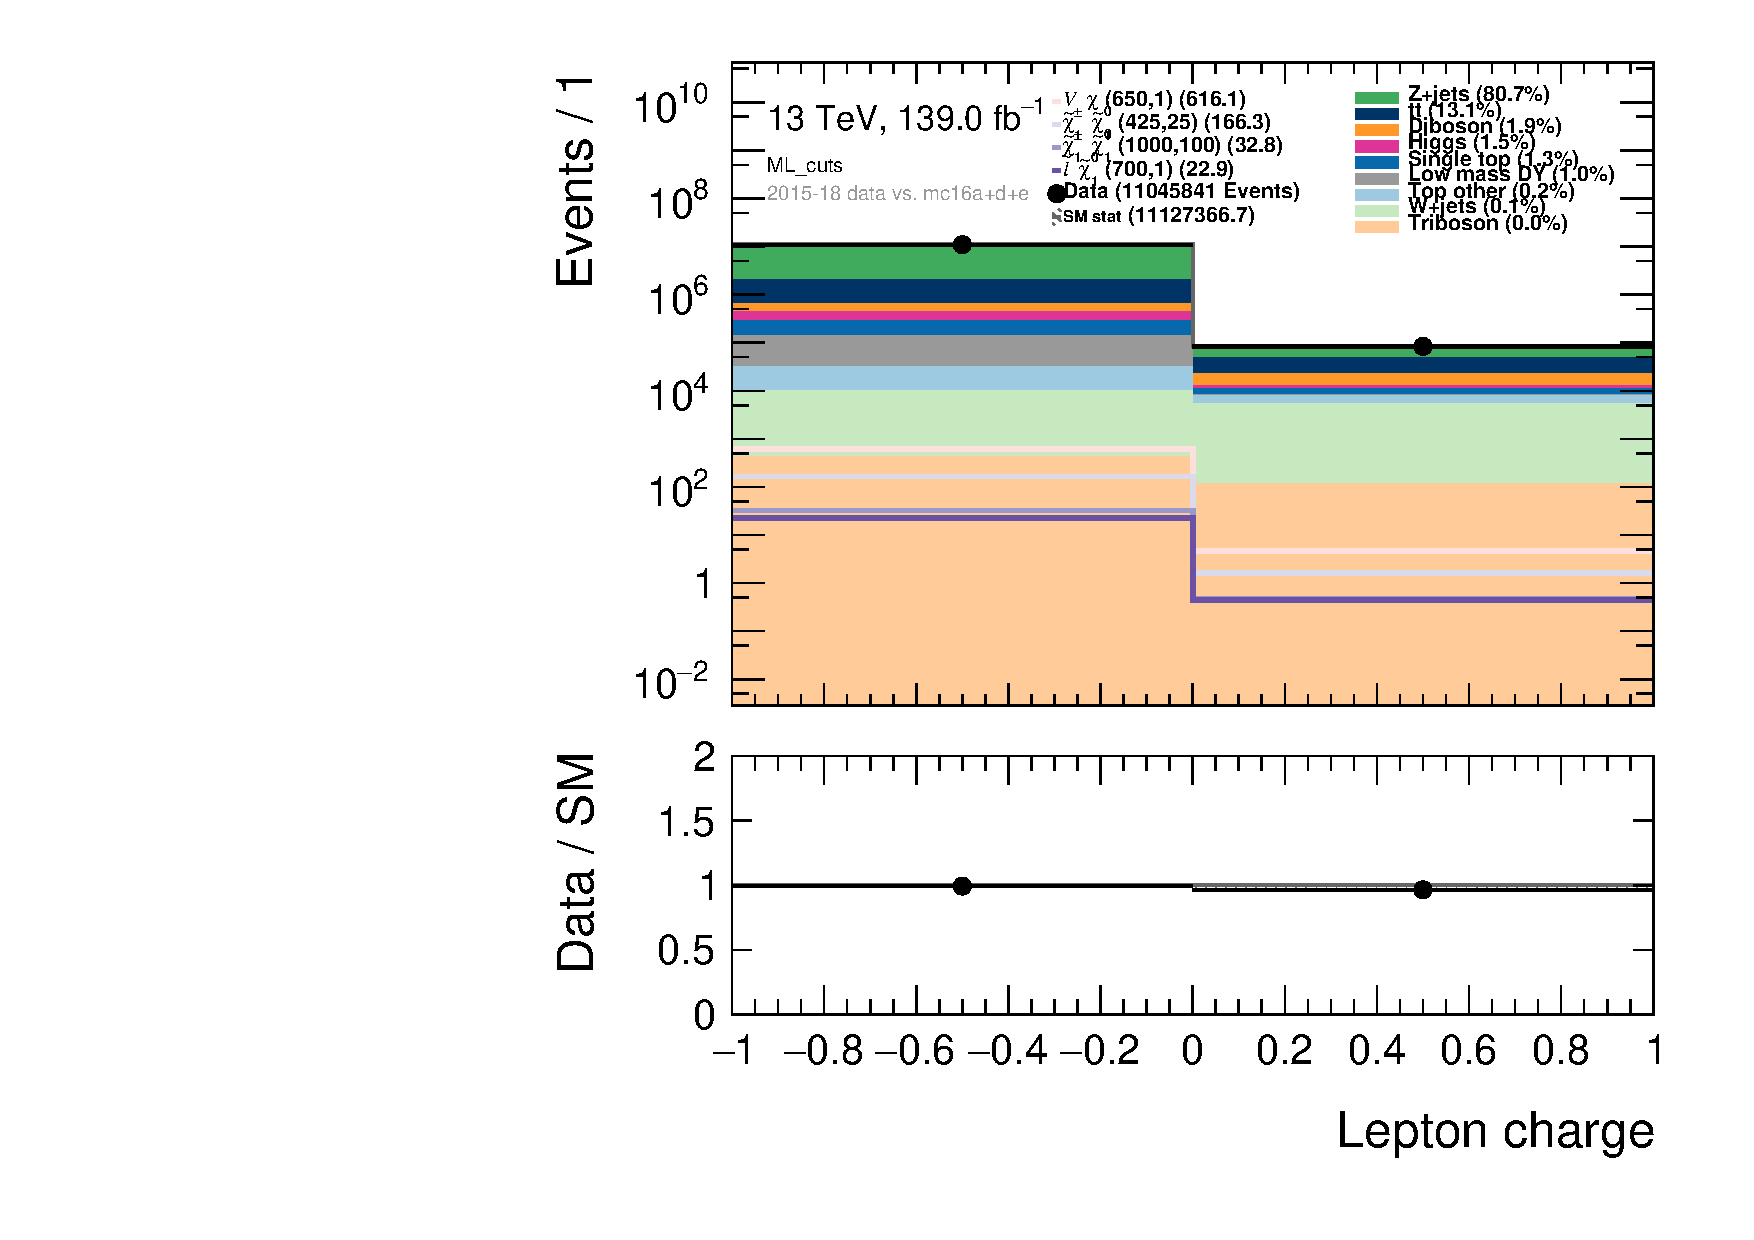
\includegraphics[width=\textwidth]{Figures/ML_cuts/hist1d_lepCharge[0]lepCharge[1]_ML_cuts.pdf}
    \caption{Events with two opposite sign (OS, first bin) and same sign (SS, second bin) leptons.}
    \label{fig:my_label}
    \end{subfigure}
    \caption{Plots of the different variables used as features in the ML algorithms after the preselection cuts in Table \ref{tab:precutsSlepSlep} have been applied.}
    \label{fig:ML_cuts}
\end{figure}


\restoregeometry

To make our ML analysis code more user friendly and unbiased (give the ML the opportunity to figure it out), we have used the same precuts for all four processes.

The goal with the ML analysis is to teach the computer to separate the signal from the background and then calculate the expected significance and compare it with the cut and count results. Since we are handling a huge amount of data and each step takes some time, we have separated some of the most time consuming steps to save some time to optimize the ML part. The first thing we did was to import all the nTuples and put them into pandas dataframes. Then we did the precuts in table \ref{tab:precutsSlepSlep}, giving the dataframes the features in table \ref{tab:features}, weighting and scaling up each event to correct luminosity from table \ref{tab:eventWeights} before we in the end stored all of the processed dataframes temporarily into HDF5 files \footnote{HDF5 \cite{hdf5} is a file format to store large, complex and heterogeneous data}. To avoid huge memory issues in the computer, this is done chunk by chunk since importing the whole dataset in one go is too much for our computers to handle. 

Importing the data is the most time consuming step, but luckily we don't have to do this every time we do some adjustments which is mainly done in the next step, the ML part. In the ML part we are training two different algorithms, namely a BDT and a NN. 

As mentioned in chapter \ref{sec:ML} we have to divide our input data into train and test sets, which are done by simply taking 1/3 of the input (randomly drawn) and call it the test set. This data is not going to be touched until we are finished with the training of our model except for 1/10 of the test set which is used as a validation set. To both save some time in the training and to give the BDT and NN the opportunity to train more on actual signal samples, we have chosen to train on the same amount of background events as we have for signal. This gives us the results shown in figure \ref{fig:rawOutput}, which is the raw output from the trained model. The data sent into the ML are scaled between 0 and 1, where the MC background have gotten a label 0 and the signal a label 1. This gives us also an output between 0 and 1 which is the x-axis in \ref{fig:rawOutput}. Looking at the raw output gives us a good indication on how little MC background we need during training to obtain the results we have in this thesis and have made the training a lot less time consuming. The reduction of the background does not have much impact on the results for the BDT except for some reduced training time, but for the NN the results improves a lot by doing this. 


\begin{figure}[H]
    \centering
    \begin{subfigure}[t!]{0.49\textwidth}
        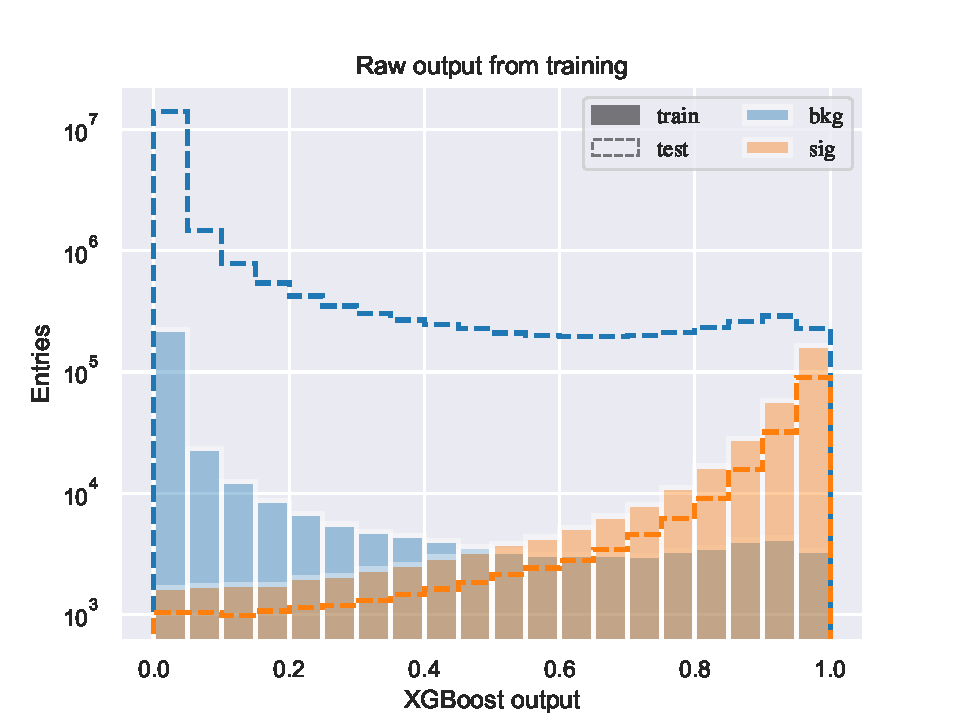
\includegraphics[width = \textwidth]{Figures/SlepSlep/ML/BDT/All_level/Low/rawPlot.pdf}
        \caption{A plot of the raw output from the BDT.}
        \label{fig:SlepSlepBDTLowLevelLowRaw}
    \end{subfigure}
    \begin{subfigure}[t!]{0.49\textwidth}
        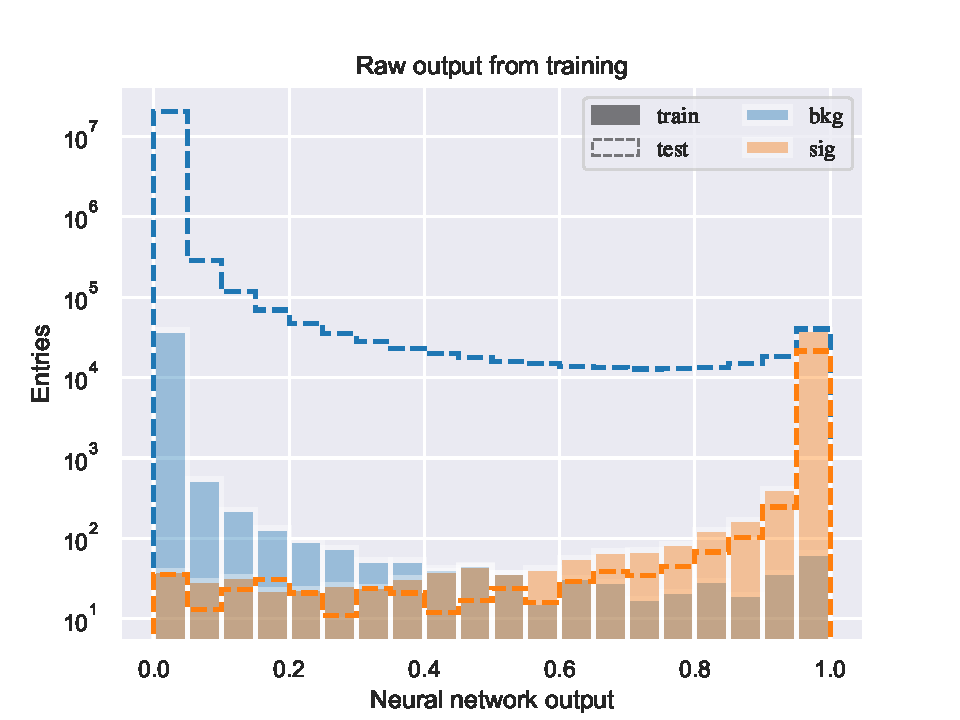
\includegraphics[width = \textwidth]{Figures/SlepSlep/ML/NN/All_level/High/rawPlot.pdf}
        \caption{A plot of the raw output from the NN.}
        \label{fig:SlepSlepNNLowLevelHighRaw}
    \end{subfigure}
    \caption{Examples on how the raw output from a BDT (left) and NN (right) look after training and testing. This is obtained by using the signal samples from direct slepton production with low mass splitting and all level variables. These plots look very similar for all of the different signal processes and trained model and are therefore only these are shown here.}
    \label{fig:rawOutput}
\end{figure}



Since one signal sample alone is pretty small, we have merged the signal samples into different mass splittings for each process. The reason for this is that with several samples together we get a lot more data to train our BDT and NN on and in this way our model will also handle other datasets much better. The mass splittings are defined by the lines drawn in figure \ref{fig:exclusionPlots} in chapter \ref{sec:CandCanalysis}. This gives us the mass splittings as shown in table \ref{tab:massSplittings} for each process.

\begin{table}[H]
    \centering
    \renewcommand{\arraystretch}{1.3}
    \begin{tabular}{c c c c}
    \toprule
        \textbf{Process} & \textbf{Low} & \textbf{Intermediate} & \textbf{High}\\
        \midrule
        \midrule
        Direct slepton production & $\Delta$m $\leq$ 100 GeV & 100 $<$ $\Delta$m $<$450 GeV & $\Delta$m $\geq$ 450 GeV\\
        Chargino production via $\Tilde{l}/\Tilde{\nu}$& $\Delta$m $<$ 200 GeV & 200 $\leq$ $\Delta$m $<$600 GeV & $\Delta$m $\geq$ 600 GeV\\
        Chargino production via $W^\pm$ & $\Delta$m $<$ 150 GeV & 300 $\leq$ $\Delta$m $<$300 GeV & $\Delta$m $\geq$ 300 GeV\\
        Mono-Z & $\Delta$m $<$ 100 GeV & 100 $\leq$ $\Delta$m $<$350 GeV & $\Delta$m $\geq$ 350 GeV\\
        \bottomrule
    \end{tabular}
    \caption{Table defines the different mass splittings based on figure \ref{fig:exclusionPlots} for the different processes.}
    \label{tab:massSplittings}
\end{table}

%What signal sample that is in which category can also be found in the tables in \ref{sec:sigsamptab}.

When training the ML models we have different means for evaluating how good or bad the models are doing. We can for example scale the test set up to be as big as the training set to see how good the fit between the up-scaled training and testing sample is, shown in figure \ref{fig:traintestscaledExample}. We can also look at the ROC curve and AUC score, figure \ref{fig:ROCExample}, to see how well the model can classify background as background and signal as signal. The goal in figure \ref{fig:traintestscaledExample} is that the test set (dotted line) is matching the training set (filled bins) and in figure \ref{fig:ROCExample} we want an AUC-score close to 1.

\begin{figure}[H]
    \centering
    \begin{subfigure}[t!]{0.49\textwidth}
        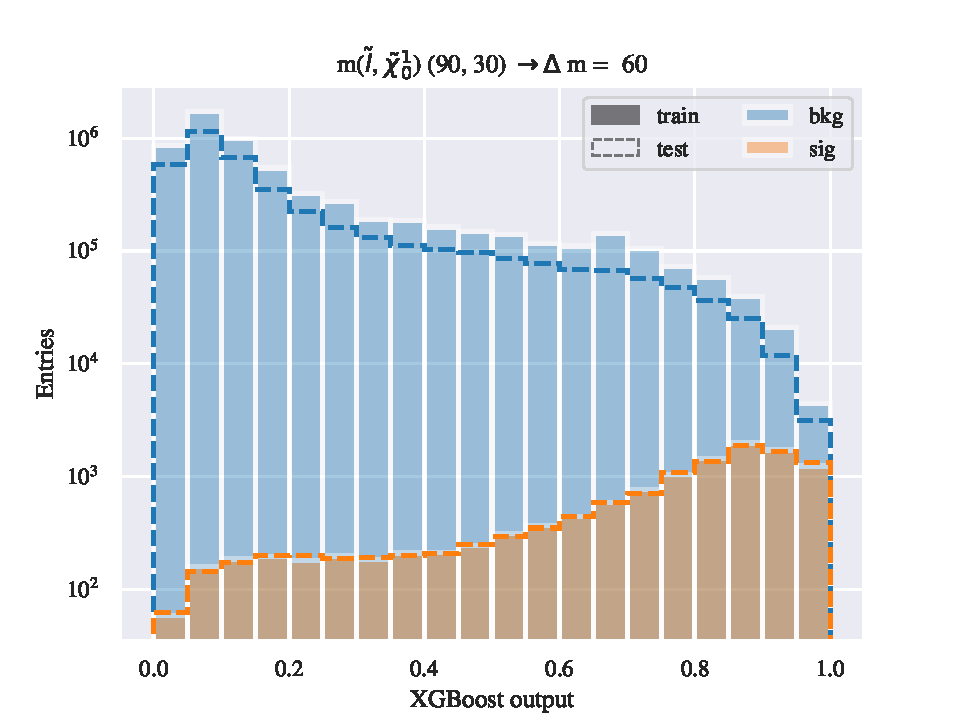
\includegraphics[width = \textwidth]{Figures/SlepSlep/ML/BDT/Low_level/Low/scaled_train_test_395897.pdf}
        \caption{A plot of the training and test set, where the test set is scaled up to match the training set.}
        \label{fig:traintestscaledExample}
    \end{subfigure}
    \begin{subfigure}[t!]{0.49\textwidth}
        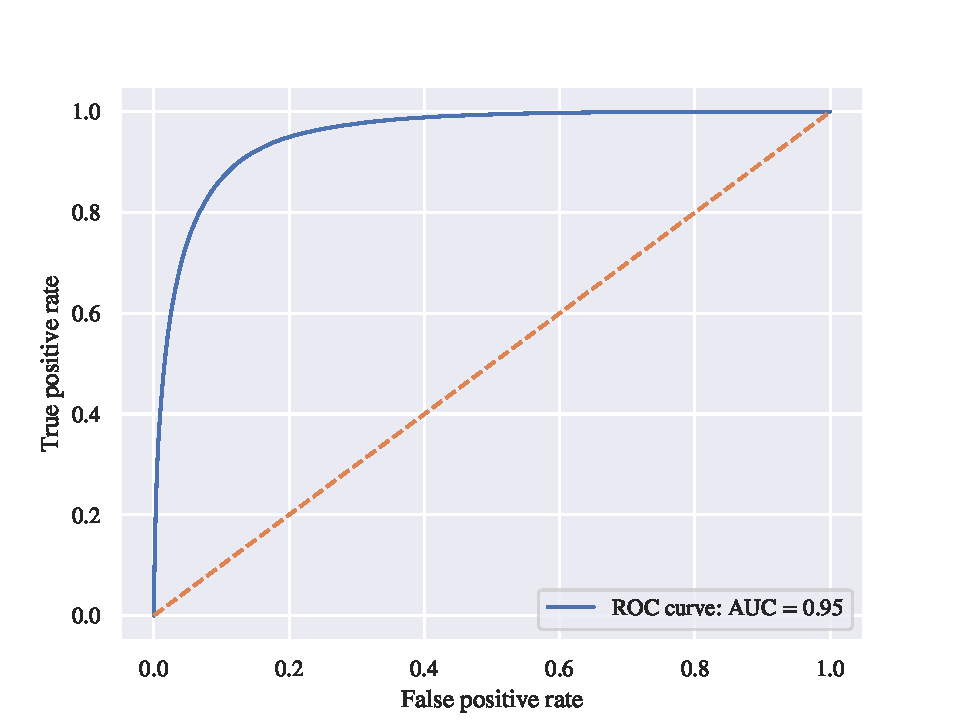
\includegraphics[width = \textwidth]{Figures/SlepSlep/ML/BDT/Low_level/Low/ROCcurve.pdf}
        \caption{A plot of the ROC curve together with the AUC score.}
        \label{fig:ROCExample}
    \end{subfigure}
    \caption{In this figure you can see results from a BDT trained on low mass splittings and with low level features for the direct slepton production.}
    \label{fig:resExample}
\end{figure}

Both of the plots in figure \ref{fig:resExample} are merely shown to illustrate what we are judging the training on. The ROC-curve will not be shown for every trained model, but the AUC-score will be presented in a table for every trained model. For reference later in the results, we say that an AUC-score $\gtrsim 0.85$ is a good score.

In addition to the ROC-curve and AUC-score, we have plotted the training loss vs the validation loss and the training accuracy vs the validation accuracy for the NN as shown in figure \ref{fig:resLossAccExample}. The loss should go towards zero and the accuracy towards one. 

\begin{figure}[H]
    \centering
    \begin{subfigure}[t!]{0.49\textwidth}
        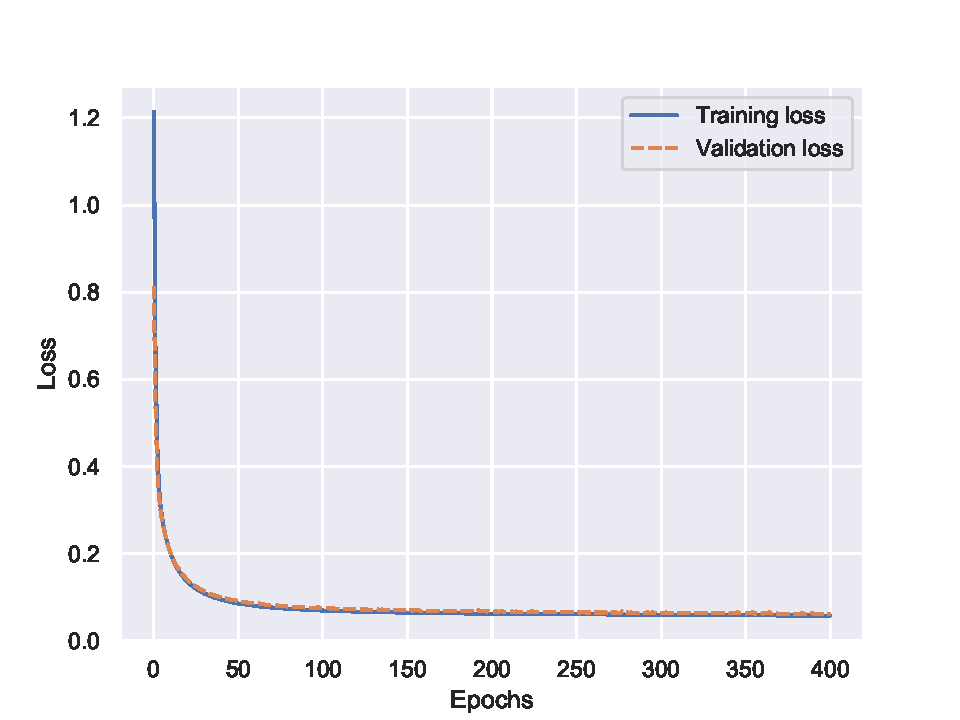
\includegraphics[width = \textwidth]{Figures/SlepSlep/ML/NN/High_level/Inter/Loss_sig_slepslep_high_level_high.pdf}
        \caption{A plot of the training loss vs the validation loss.}
        \label{fig:LossExample}
    \end{subfigure}
    \begin{subfigure}[t!]{0.49\textwidth}
        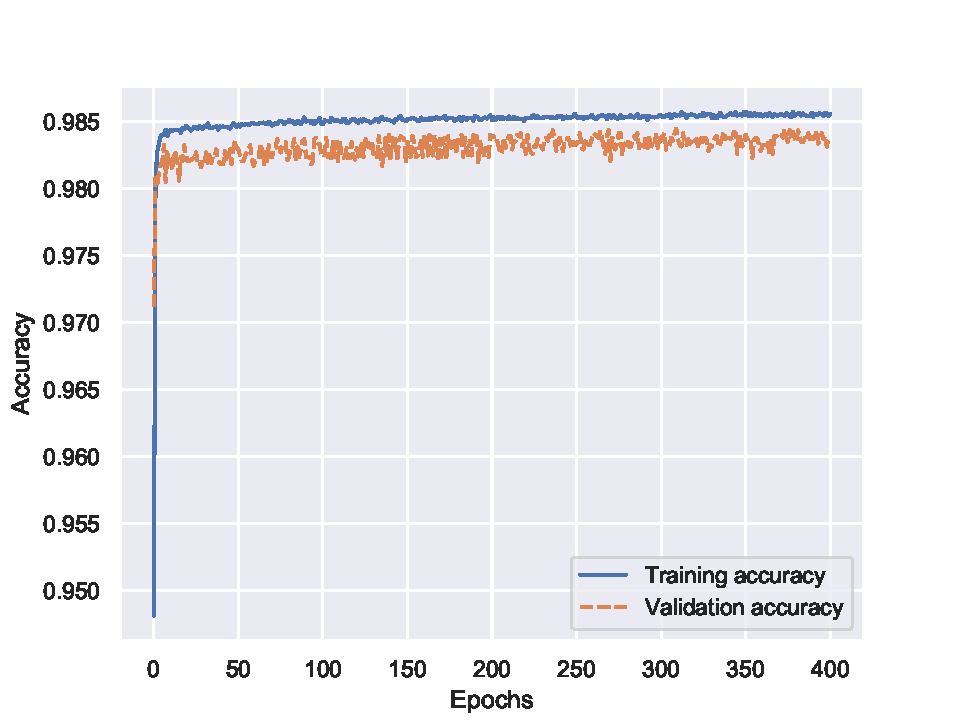
\includegraphics[width = \textwidth]{Figures/SlepSlep/ML/NN/High_level/Inter/Accuracy_sig_slepslep_high_level_high.pdf}
        \caption{A plot of the training accuracy vs validation accuracy.}
        \label{fig:AccExample}
    \end{subfigure}
    \caption{In this figure we can see results from a NN trained on high mass splittings and with high level variables for the direct slepton production.}
    \label{fig:resLossAccExample}
\end{figure}

As we can see in figure \ref{fig:LossExample}, both the training and validation losses goes quickly towards zero after the NN starts training and does not improve much after $\sim 100$ epochs. This means that we probably could have stopped the training after only 100 epochs and would still have gotten a fairly good result, but we want the best result as possible and therefore we let it minimize the loss further. We can also see that the validation loss is completely flat in the end and would not improve further (continue towards zero), while the training loss continues down towards zero (this is not that easy to see because of the scale on the y-axis, but nice to follow during training where you can see the loss for each epoch). Let us say we have given the NN a patience on 50 epochs instead of 10, we would most likely see that the validation loss would tend to move away from zero. This is not that easy to see in this plot, but same point is in the accuracy plot in figure \ref{fig:AccExample}, where we can see this more clearly. It is a bit hard to determine if the validation accuracy tends to go down again because of the fluctuations\footnote{The fluctuations can be avoided by having a bigger validation set, but then you will also have a smaller test set to test our ML model on.}, but it is fairly easy to see that the training accuracy continue towards one. That the training loss and accuracy continues to improve is often due to overtraining/overfitting which we want to avoid.

The plots in figure \ref{fig:resLossAccExample} for every process will not be presented in this thesis since they are going to look very similar for every process and ensemble of training compositions. All of the results that are not included in this thesis or the appendix can be found in the GitHub repository \url{https://github.com/monaanderssen/MasterML} together with the ML code.


\section{Building, training and testing the BDT}
Now we know how a BDT and NN works and we are aware of the results to expect. In this section we will get an understanding on how the BDT is built up, how we train it and, in the end, testing how well the training went.

\subsection{Building}
The BDT, as mentioned in chapter \ref{sec:BDT}, is built up using an existing python library called XGBoost. The hyperparameters of the method are listed in table \ref{tab:parametersBDT} below. 

\begin{table}[H]
    \centering
    \renewcommand{\arraystretch}{1.}
    \begin{tabular}{c c}
    \toprule
    \textbf{Parameter} & \textbf{Value}\\
    \midrule
    \midrule
    Maximum depth of tree & 3\\
    Learning rate     & 0.1 \\
    Number of estimators     & 10000000\\
    Verbosity & 3\\
    Objective & binary:logistic\\
    Scale position weight & 1\\
    \bottomrule
    \end{tabular}
    \caption{An overview of the different parameters used during training to obtain the results for the BDT.}
    \label{tab:parametersBDT}
\end{table}

Most of these parameters are self explanatory, but not all of them so we will take a brief explanation before we move on. The first parameter that is not so intuitive is the verbosity level, which we set to let the BDT know how much information we want from the tree during training. This can be set to 0, 1, 2 or 3, where 0 is silent, 3 is debug and 1 and 2 will give us parts of the information. It is nice to see what is going on during the training, so we have chosen to set it to 3. The next parameter is the objective, which specifies the learning task we are doing and the learning objective. As we can see in table \ref{tab:parametersBDT}, we have chosen to use something called \texttt{binary:logistic} which simply is a logistic regression for a binary classification. And last, we have the scale position weight which controls the balance between negative and positive weights in the tree. These parameters are chosen by simply trial and error (especially depth of tree and learning rate), and they are optimized for the direct slepton production process.

In addition to the parameters that we have to give to the BDT, we have different compositions of models we are training. As mentioned earlier in this chapter we are training on three different mass splittings (low, intermediate and high), but we are also training on high level, low level or all the features we listed up in table \ref{tab:features}. This is done to see how important the different features are during the next step, namely the training.

\subsection{Training}
While we train our BDT, we have to be aware of overtraining/overfitting. This can easily be done by putting in a demand on the loss and stop the training early. This is simply done by calculating the loss from the validation set and give the BDT a patience parameter of 20 steps which means that it will stop if the loss has not improved in 20 steps, and save the model made at the best iteration. This is also the reason for the high number of estimators in table \ref{tab:parametersBDT}.

It is not much more we can do while the BDT is training, other than wait to see how the testing looks. If we are not happy with how the model is trained, we have to go back to the building of the tree and adjust the parameters in table \ref{tab:parametersBDT} and do the training again until we are happy with our results.

\subsection{Testing}
The last step of the BDT is to test it on the test set. We have a lot of results from the BDT to look at since we have trained the model with low, intermediate and high mass splittings and with high level, low level and all features for four different processes. We are going to look at all four processes at the same time and see how the results evolves when changing the features and mass splittings. All the results which are not shown in this chapter can be found in the appendix \ref{sec:appBDTplots}. 

\subsubsection{AUC score}
The main selection of results is done based on the AUC-score. If the AUC-score is the same for high level, low level and all features, we have made the selection on looking at which features that have been important for the trained model. The AUC-scores are listed in table \ref{tab:AUCBDT}. 

\begin{table}[H]
    \centering
    \renewcommand{\arraystretch}{1.}
    \begin{tabular}{l l c c c c }
    \toprule
    \textbf{Level} & $\mathbf{\Delta m}$ & $\mathbf{\Tilde{l} \Tilde{l}}$ & $\mathbf{\Tilde{\chi}_1^\pm \rightarrow \Tilde{l}/\Tilde{\nu}}$ & $\mathbf{\Tilde{\chi}_1^\pm \rightarrow W^\pm}$ & \textbf{Mono-Z}  \\
    \midrule
    \midrule
    \multirow{3}{*}{High} &  Low   & 0.91 & 0.91 & 0.91 & 0.95 \\
     & Intermediate & 0.99 & 0.98 & 0.94 & 0.96 \\
     & High & 1.00 & 1.00 & 0.96 & 0.97 \\
     \midrule
    \multirow{3}{*}{Low} & Low & 0.95 & 0.93 & 0.93 & 0.95 \\
     & Intermediate & 0.99 & 0.98 & 0.95 & 0.97 \\
     & High & 1.00 & 1.00 & 0.97 & 0.97 \\
     \midrule
    \multirow{3}{*}{All} & Low & 0.97 & 0.95 & 0.94 & 0.96 \\
     & Intermediate & 1.00 & 0.99 & 0.96 & 0.97 \\
     & High & 1.00 & 1.00 & 0.98 & 0.98 \\
     \bottomrule
    \end{tabular}
    \caption{The AUC score for all four processes with different compositions of features and mass splittings for the BDT.}
    \label{tab:AUCBDT}
\end{table}


As we can see in table \ref{tab:AUCBDT}, the preferred composition of features is in most cases to use all the features, except for some few exceptions where all three options have the same AUC-score. As mentioned above, this is then determined by looking at the feature importance plot that also are presented in the following sections. The results are presented for each mass splitting with all the processes together for easier comparison. The signal samples shown here are the same as we looked at in the cut and count analysis presented in chapter \ref{sec:CandCanalysis}.
















\subsubsection{Low mass splittings}
The first results presented is for the BDTs trained on low mass splittings. The preferred composition of features is all features and in figure \ref{fig:AllLowfeatBDT} we can see how these different features contributes during training. 


\begin{figure}[H]
    \centering
    \begin{subfigure}[t!]{0.49\textwidth}
        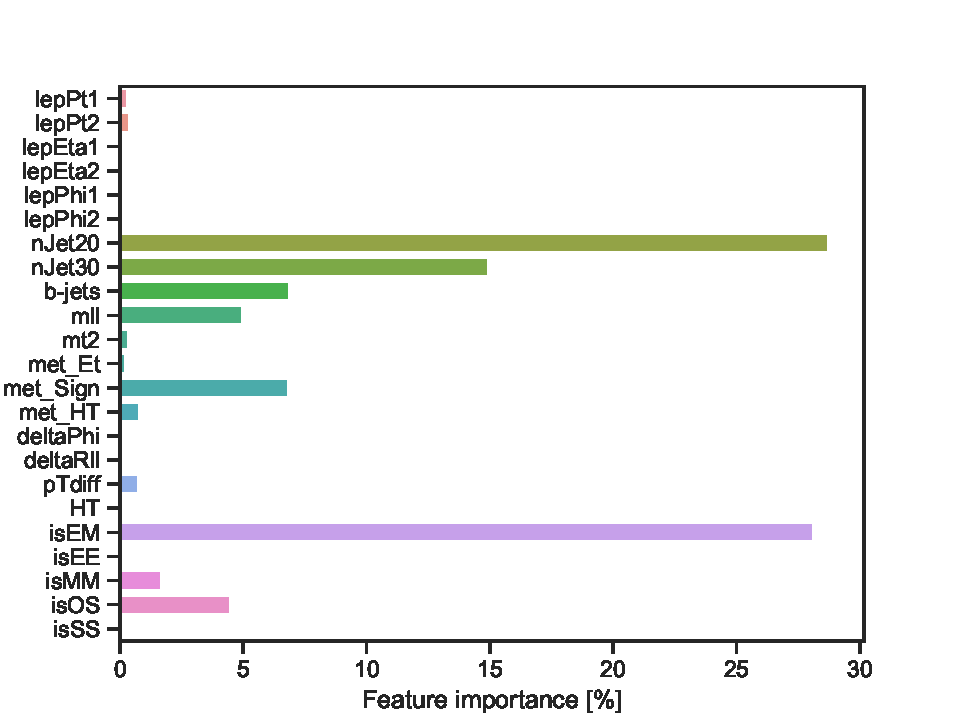
\includegraphics[width = \textwidth]{Figures/SlepSlep/ML/BDT/All_level/Low/featureImportance.pdf}
        \caption{Direct slepton production.}
        \label{fig:featSlepslepLow}
    \end{subfigure}
    \begin{subfigure}[t!]{0.49\textwidth}
        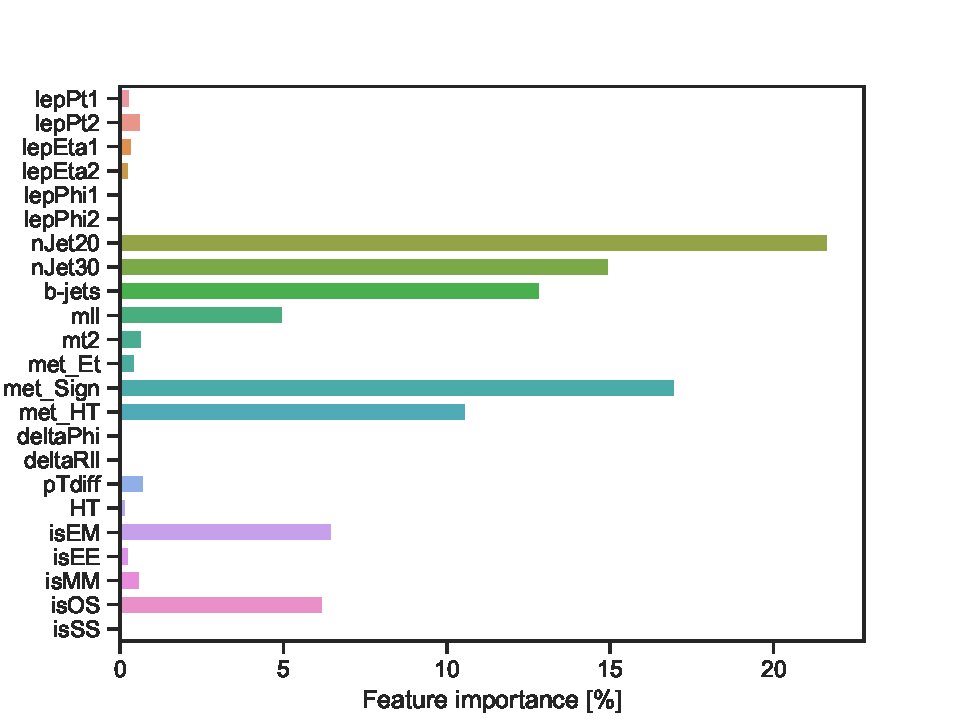
\includegraphics[width = \textwidth]{Figures/SlepSnu/BDT/All_level/Low/featureImportance.pdf}
        \caption{Chargino production via $\Tilde{l}/\Tilde{\nu}$.}
        \label{fig:featSlepsnuLow}
    \end{subfigure}
    \begin{subfigure}[t!]{0.49\textwidth}
        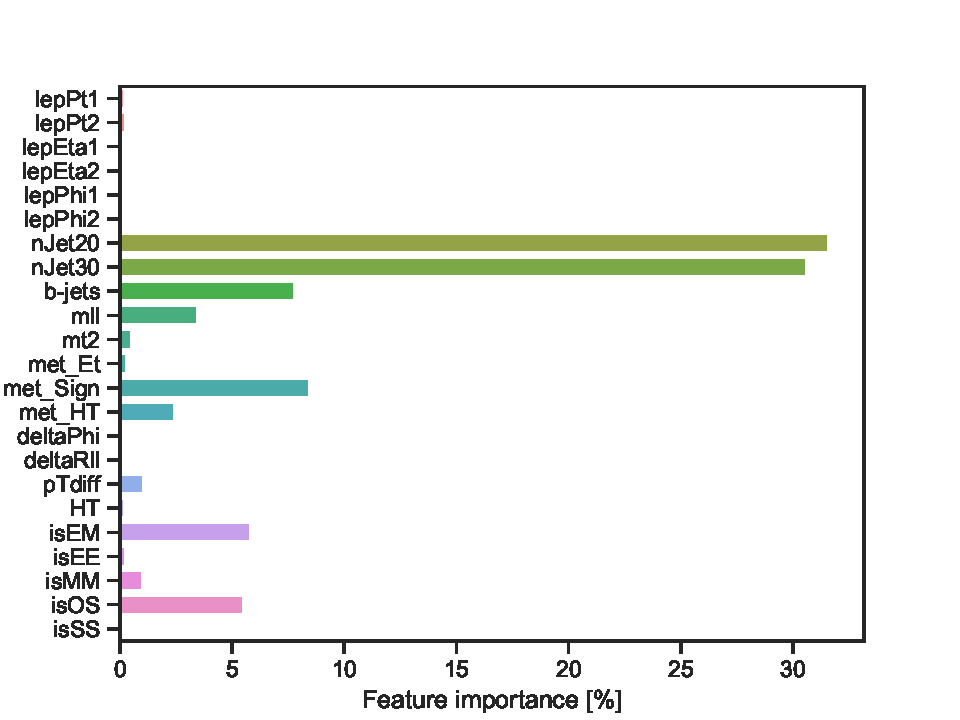
\includegraphics[width = \textwidth]{Figures/WW/BDT/All_level/Low/featureImportance.pdf}
        \caption{Chargino production via $W^\pm$.}
        \label{fig:featWWLow}
    \end{subfigure}
    \begin{subfigure}[t!]{0.49\textwidth}
        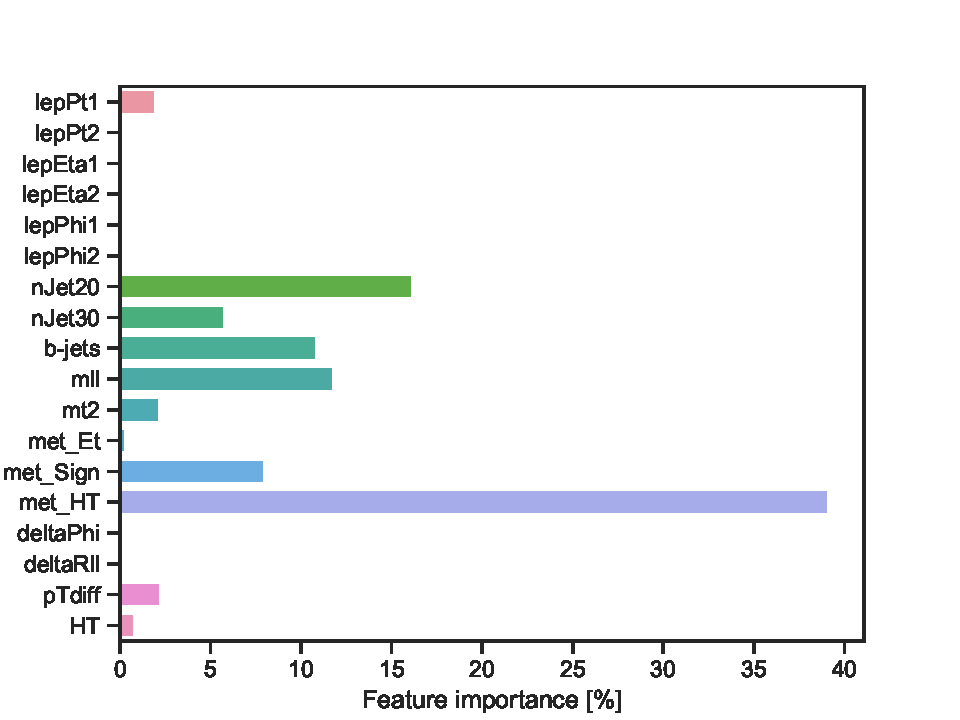
\includegraphics[width = \textwidth]{Figures/Mono_Z/ML/BDT/All_level/Low/featureImportance.pdf}
        \caption{Mono-Z.}
        \label{fig:featMonoZLow}
    \end{subfigure}
    \caption{Feature importance for low mass splittings for all four processes using all features during training.}
    \label{fig:AllLowfeatBDT}
\end{figure}

If we now look at the different feature contributions in figure \ref{fig:AllLowfeatBDT}, we can see that jets with a $p_T > 20$ GeV is an important feature when the BDT is trained on SUSY processes. This means that the BDT evaluate this as a powerful variable to distinguish signal from background. This is in accordance with the cut and count analysis where a cut on jets is applied. In addition we can see that the jets with a $p_T > 30$ GeV, b-jets, $m_{ll}$ and MET significance have been used a lot. These are the variables we used in the cut and count analysis, but they do not contribute equally much for every SUSY process. For the mono-Z process the same features as for the SUSY processes are used, however, MET/$H_T$ is regarded as the second most important one. This again is reflected in the cut and count analysis where a cut on this variable is applied. For all of the four processes the tree finds the different flavor and opposite sign variable powerful when trying to separate the signal from background. To conclude the feature importance for low mass splittings we can say that there are no big surprises when comparing with the cuts applied in cut and count analysis.

The next step is to see how well the testing of the model went. This can be seen in figure \ref{fig:AllLowBDT} below.

\begin{figure}[H]
    \centering
    \begin{subfigure}[t!]{0.49\textwidth}
        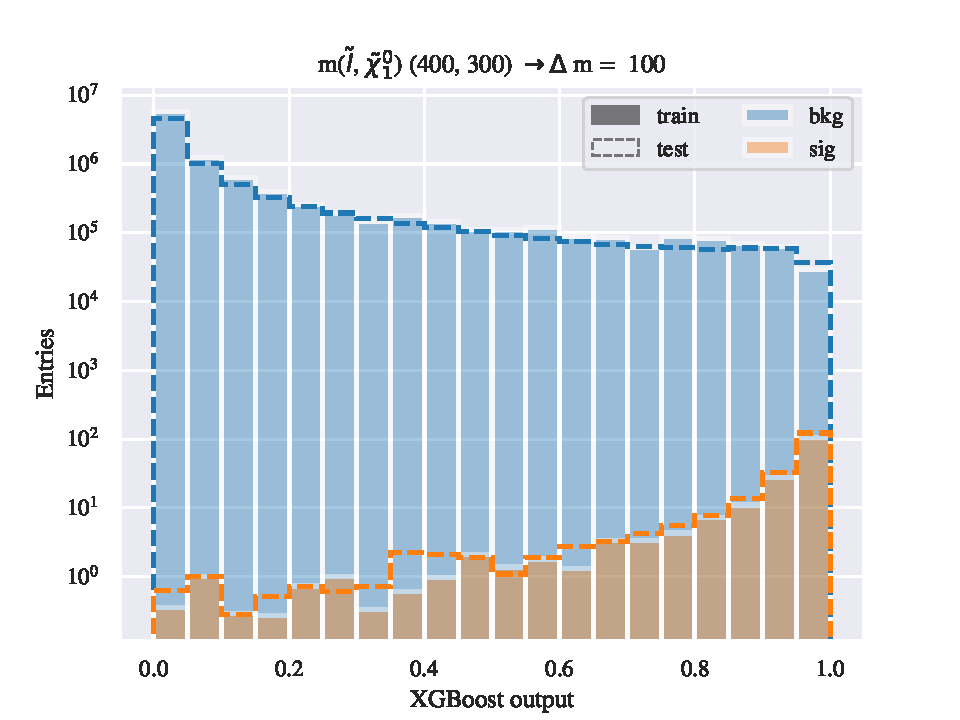
\includegraphics[width = \textwidth]{Figures/SlepSlep/ML/BDT/All_level/Low/scaled_train_test_395984.pdf}
        \caption{Direct slepton production.}
        \label{fig:SlepslepLow}
    \end{subfigure}
    \begin{subfigure}[t!]{0.49\textwidth}
        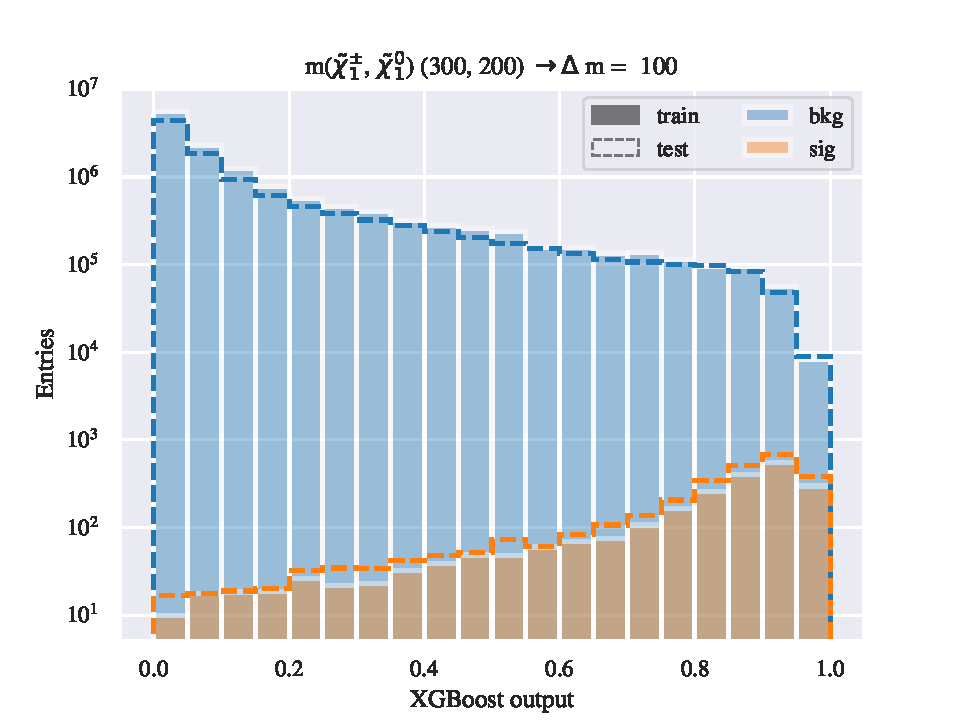
\includegraphics[width = \textwidth]{Figures/SlepSnu/BDT/All_level/Low/scaled_train_test_397115.pdf}
        \caption{Chargino production via $\Tilde{l}/\Tilde{\nu}$.}
        \label{fig:SlepsnuLow}
    \end{subfigure}
    \begin{subfigure}[t!]{0.49\textwidth}
        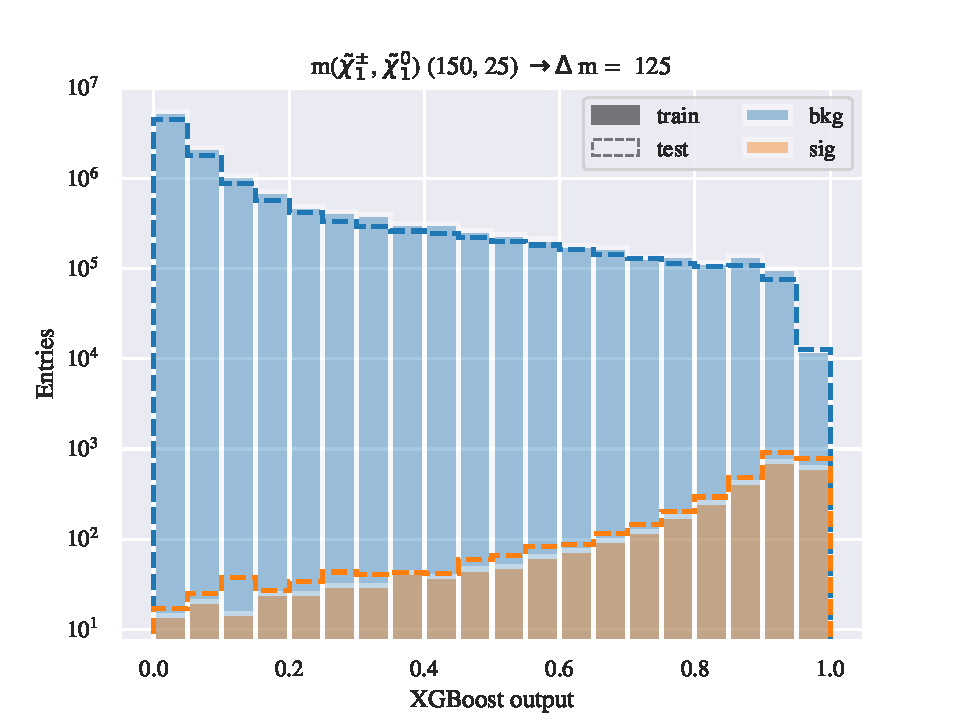
\includegraphics[width = \textwidth]{Figures/WW/BDT/All_level/Low/scaled_train_test_395268.pdf}
        \caption{Chargino production via $W^\pm$.}
        \label{fig:WWLow}
    \end{subfigure}
    \begin{subfigure}[t!]{0.49\textwidth}
        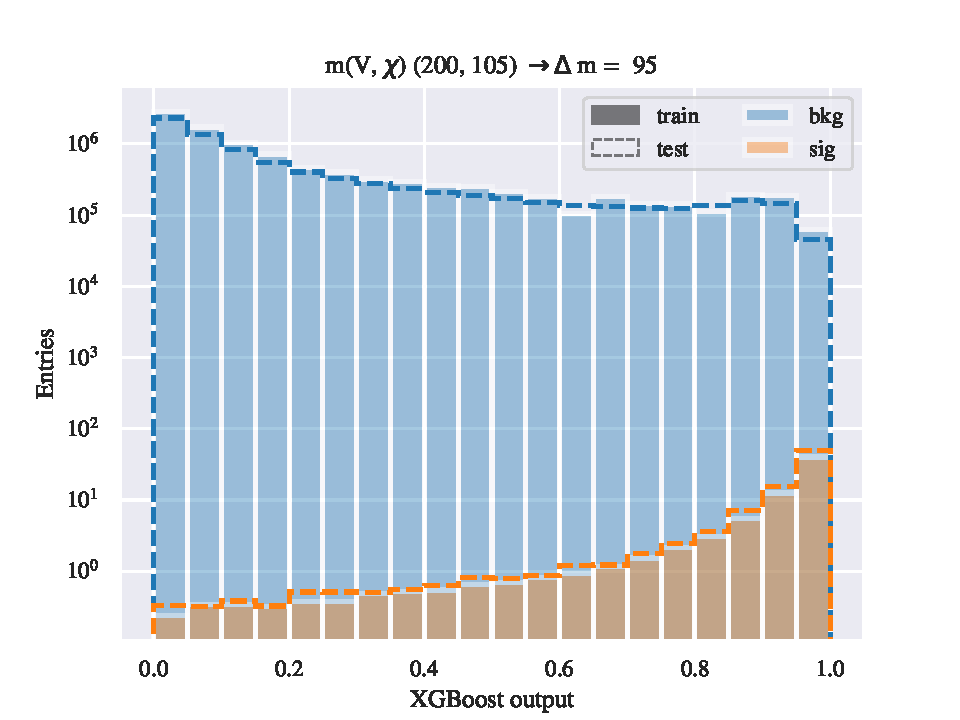
\includegraphics[width = \textwidth]{Figures/Mono_Z/ML/BDT/All_level/Low/scaled_train_test_310604.pdf}
        \caption{Mono-Z.}
        \label{fig:MonoZLow}
    \end{subfigure}
    \caption{Test vs train for low mass splittings with all features done with the BDT. Here the test set is scaled up to match the number of training events.}
    \label{fig:AllLowBDT}
\end{figure}

As we can see in figure \ref{fig:AllLowBDT}, the test set (dashed line) match the training set pretty well for all processes. It differs a bit in some places, but overall it is a good fit. We can also see that the distinction between signal and background is not that good, but it is at least most signal close to one, which is the value we have labeled the signal with. The relatively poor separation of signal and background is due to the closer of the masses of the final states particles from our signal to the masses of the particles in the SM, which makes them harder to separate. This is a major challenge in searches for new physics in high energy particle physics and is something we hope to improve in the future exploiting more advanced techniques.



























\subsubsection{Intermediate mass splittings}

The next mass splitting we are looking at is the intermediate mass splittings. In figure \ref{fig:featAllInterBDT} we can see the importance of the different features where all features are used for training. 

\begin{figure}[H]
    \centering
    \begin{subfigure}[t!]{0.49\textwidth}
        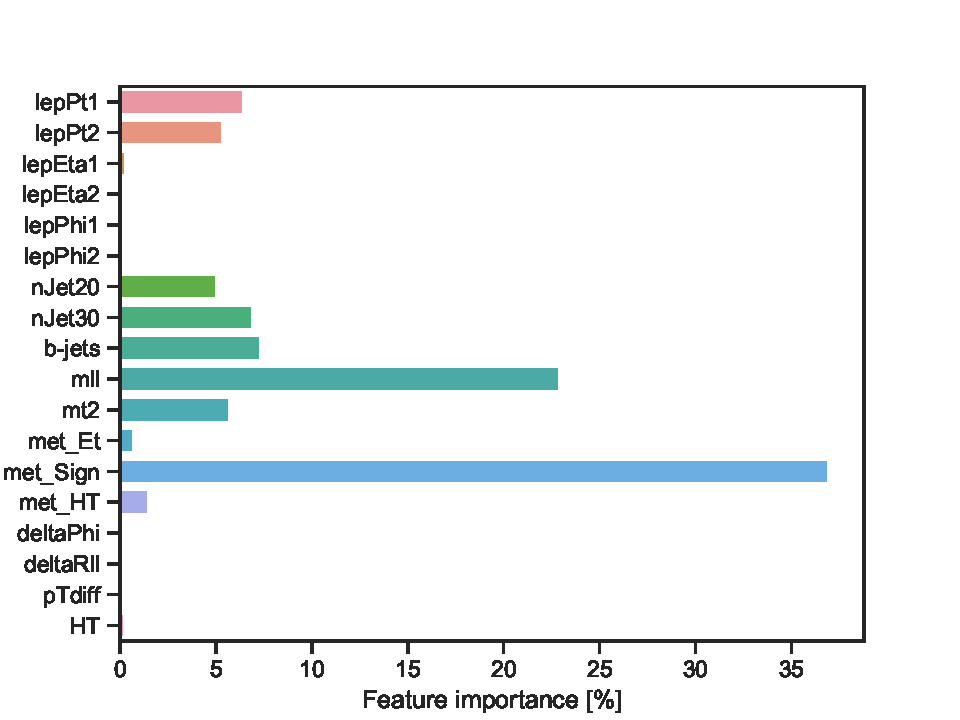
\includegraphics[width = \textwidth]{Figures/SlepSlep/ML/BDT/All_level/Inter/featureImportance.pdf}
        \caption{Direct slepton production.}
        \label{fig:featSlepslepInter}
    \end{subfigure}
    \begin{subfigure}[t!]{0.49\textwidth}
        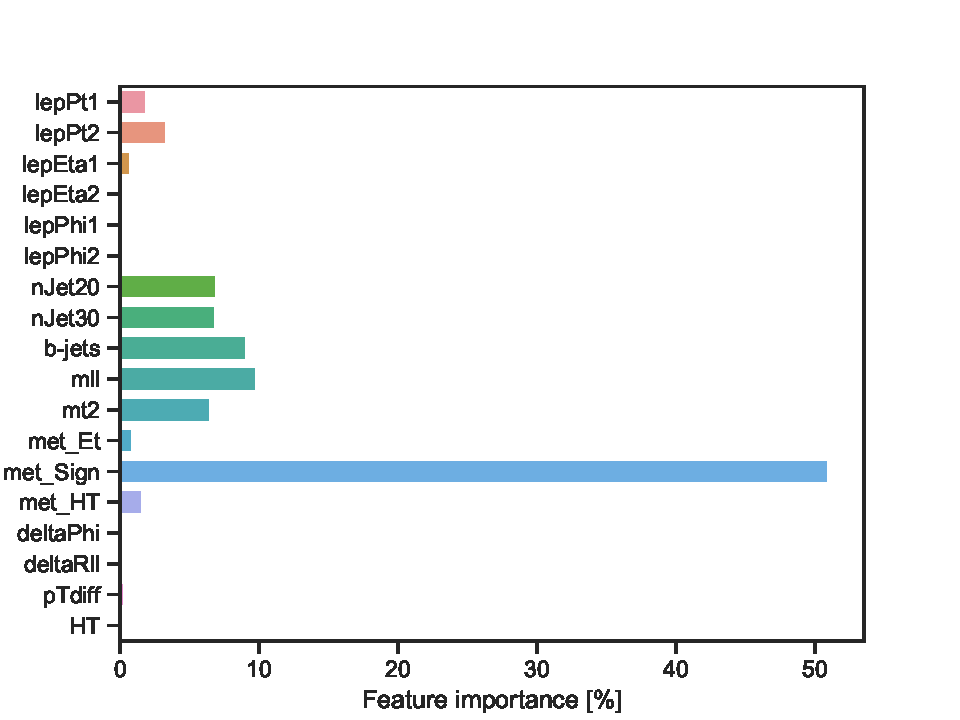
\includegraphics[width = \textwidth]{Figures/SlepSnu/BDT/All_level/Inter/featureImportance.pdf}
        \caption{Chargino production via $\Tilde{l}/\Tilde{\nu}$.}
        \label{fig:featSlepsnuInter}
    \end{subfigure}
    \begin{subfigure}[t!]{0.49\textwidth}
        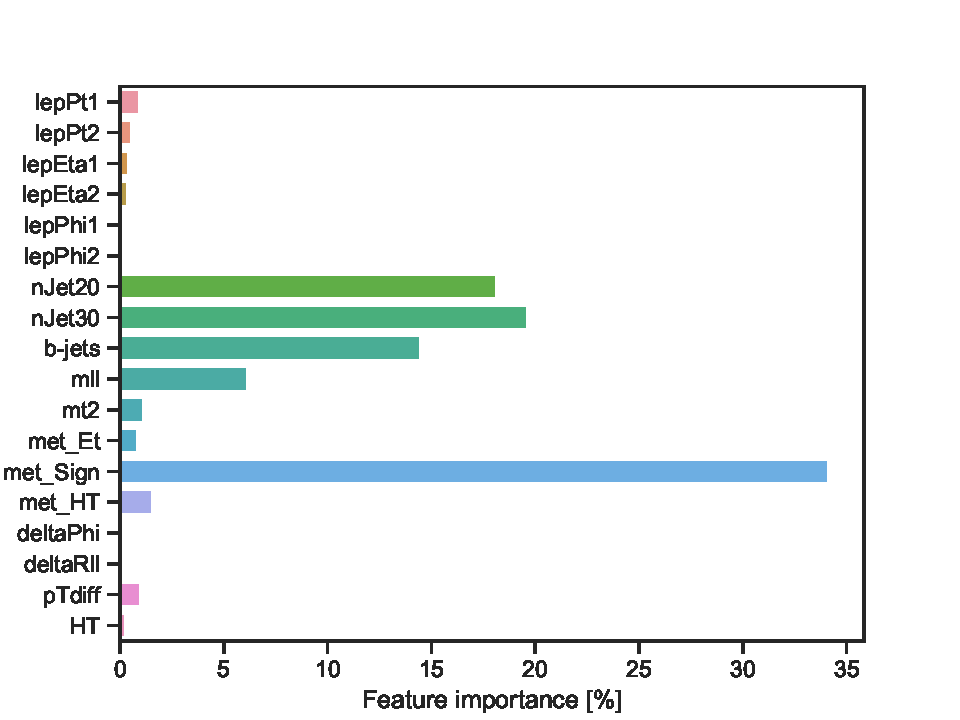
\includegraphics[width = \textwidth]{Figures/WW/BDT/All_level/Inter/featureImportance.pdf}
        \caption{Chargino production via $W^\pm$.}
        \label{fig:featWWInter}
    \end{subfigure}
    \begin{subfigure}[t!]{0.49\textwidth}
        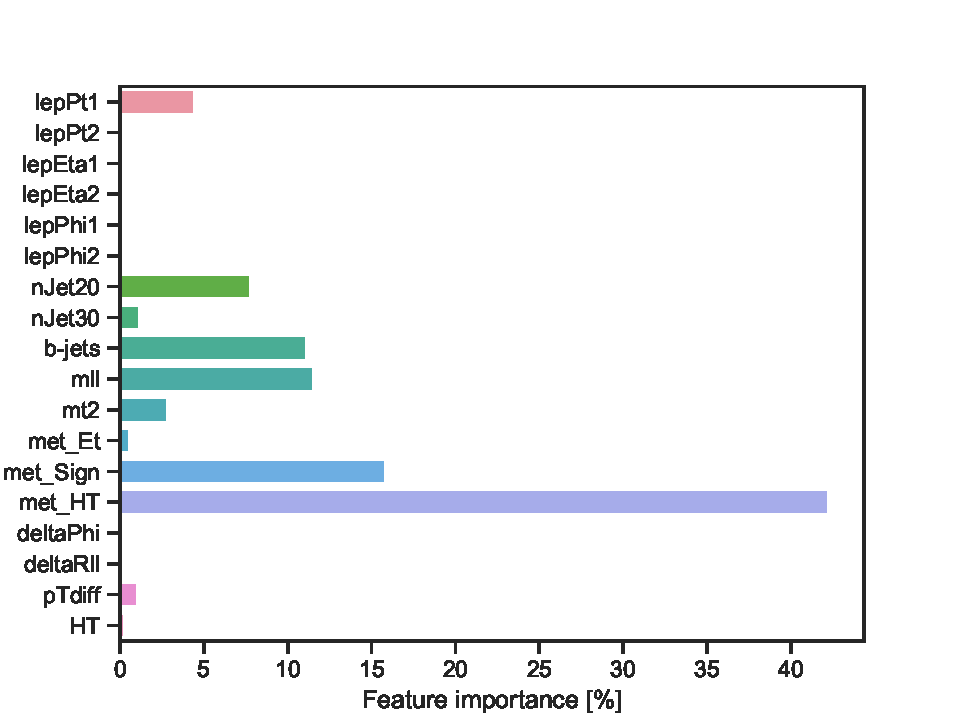
\includegraphics[width = \textwidth]{Figures/Mono_Z/ML/BDT/All_level/Inter/featureImportance.pdf}
        \caption{Mono-Z.}
        \label{fig:featMonoZInter}
    \end{subfigure}
    \caption{Feature importance for intermediate mass splittings for all four processes using all features during training.}
    \label{fig:featAllInterBDT}
\end{figure}

In figure \ref{fig:featAllInterBDT} we can see that MET significance is the most important feature for the SUSY processes and the third most important feature for mono-Z. This might be a bit more interesting result than for the low mass splittings, since we, in cut and count, do a very gentle cut on this variable while the BDT finds it very interesting in the training. For later work on a similar analysis, this could be interesting to test in the cut and count analysis as well. The other features the BDT finds interesting, for all four processes, are more or less the same as for low mass splittings. 

\begin{figure}[H]
    \centering
    \begin{subfigure}[t!]{0.49\textwidth}
        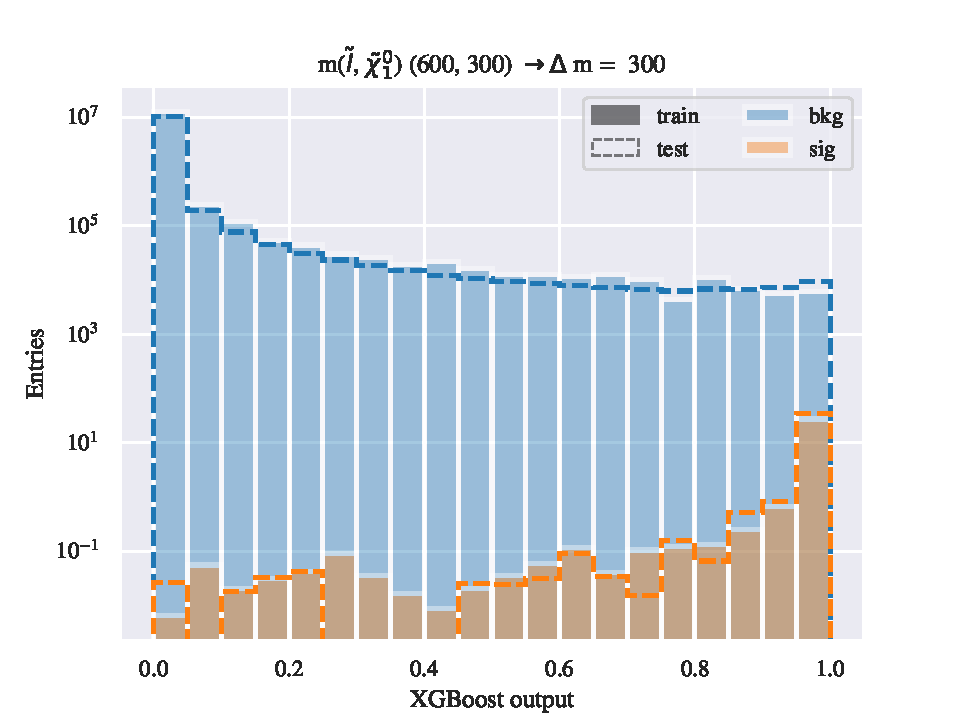
\includegraphics[width = \textwidth]{Figures/SlepSlep/ML/BDT/All_level/Inter/scaled_train_test_396014.pdf}
        \caption{Direct slepton production.}
        \label{fig:SlepslepInter}
    \end{subfigure}
    \begin{subfigure}[t!]{0.49\textwidth}
        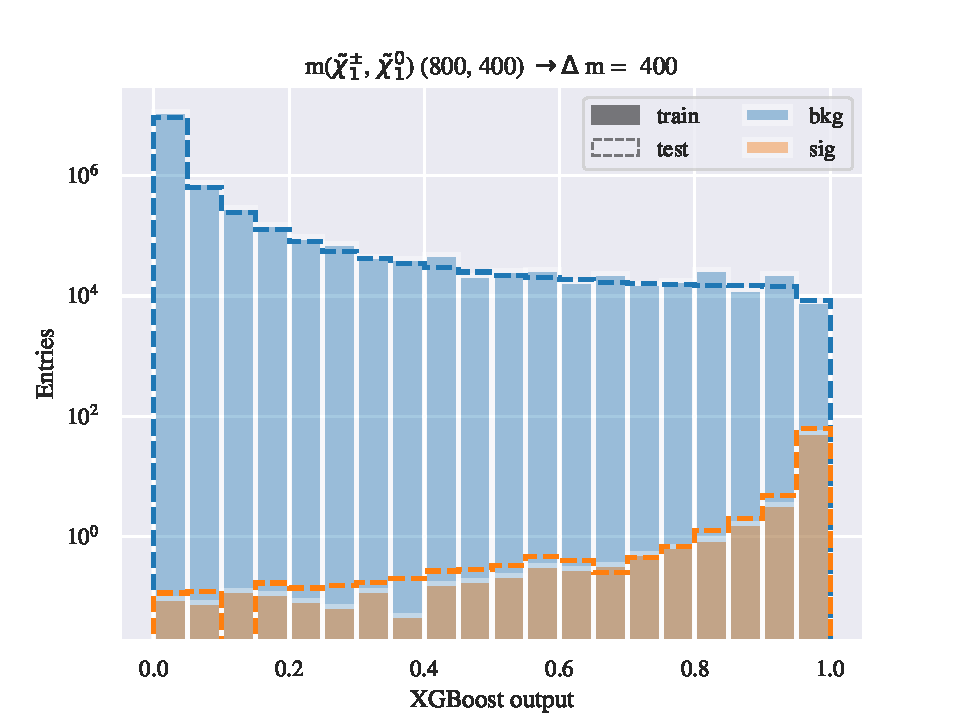
\includegraphics[width = \textwidth]{Figures/SlepSnu/BDT/All_level/Inter/scaled_train_test_397150.pdf}
        \caption{Chargino production via $\Tilde{l}/\Tilde{\nu}$.}
        \label{fig:SlepsnuInter}
    \end{subfigure}
    \begin{subfigure}[t!]{0.49\textwidth}
        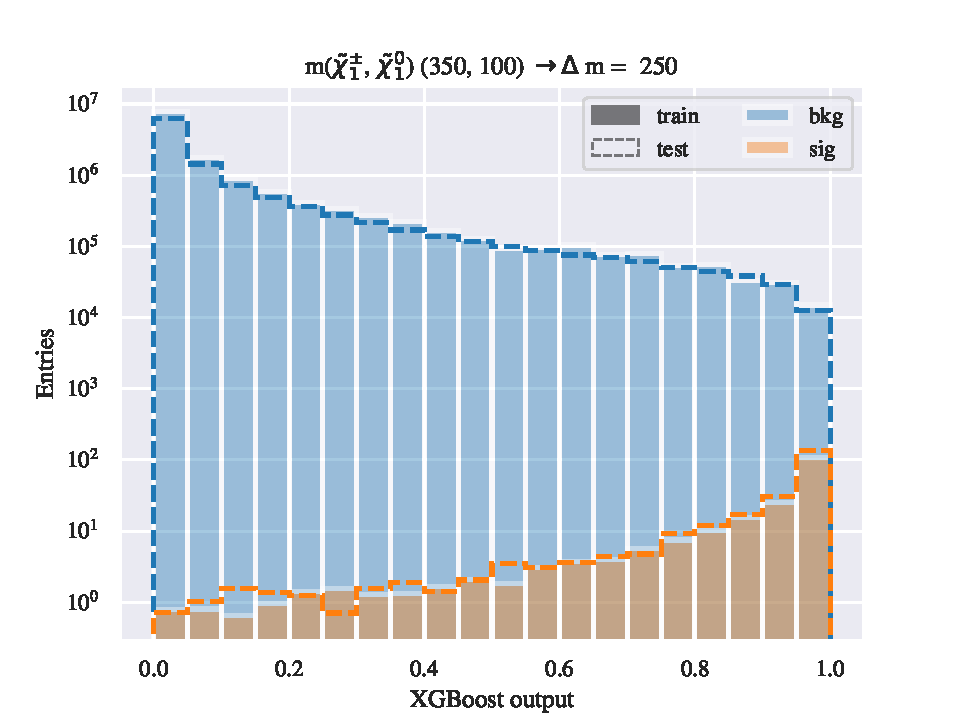
\includegraphics[width = \textwidth]{Figures/WW/BDT/All_level/Inter/scaled_train_test_395320.pdf}
        \caption{Chargino production via $W^\pm$.}
        \label{fig:WWInter}
    \end{subfigure}
    \begin{subfigure}[t!]{0.49\textwidth}
        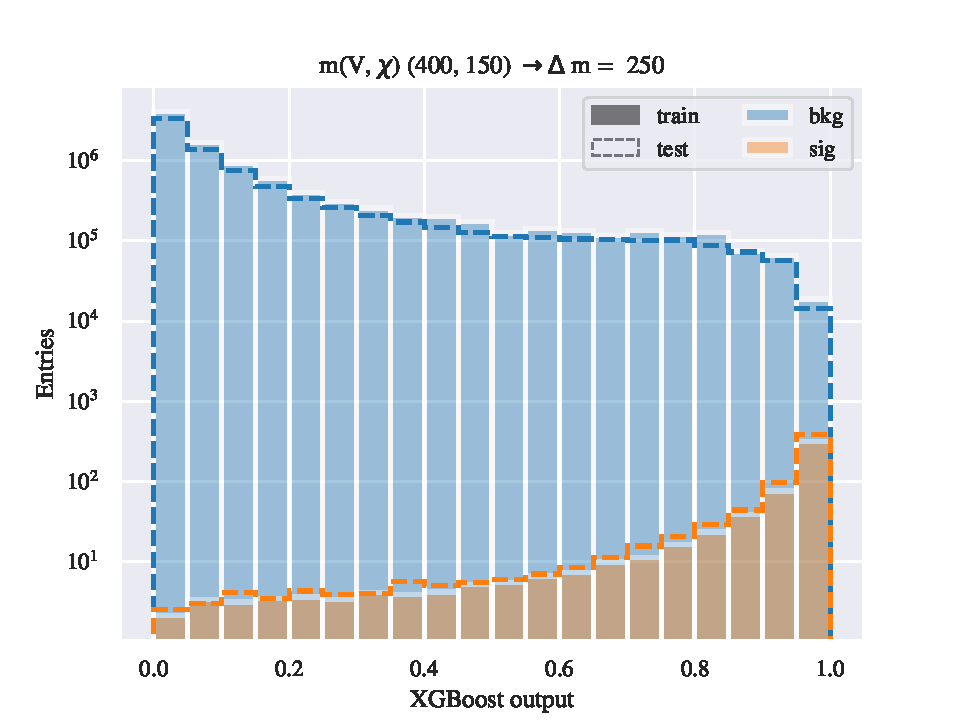
\includegraphics[width = \textwidth]{Figures/Mono_Z/ML/BDT/All_level/Inter/scaled_train_test_310613.pdf}
        \caption{Mono-Z.}
        \label{fig:MonoInter}
    \end{subfigure}
    \caption{Test vs train for intermediate mass splittings done with the BDT. Here the test set is scaled up to match the number of training events.}
    \label{fig:AllInterBDT}
\end{figure}

The results from testing the trained model is shown in figure \ref{fig:AllInterBDT}. As we could see for the low mass splittings, it is overall a pretty good match except for a couple of bins in figure \ref{fig:SlepslepInter}. Here we can see that some of the bins are lacking some background, but the test has managed to do a pretty good fit anyway. This is a result of limited statistics in the training set since it should match the amount of signal you have available. Therefore the training set is subject to statistical fluctuations. In the signal it is a bit more fluctuations and train and test does not have that good compliance. We can also see that we have a bit more signal close to one and a bit less background in this region. This is not that surprising considering that we are in a region where our final state particles have typical masses larger than the SM particles. 
















\subsubsection{High mass splittings}

The last BDT we have trained is the one on high mass splittings. Figure \ref{fig:AllHighfeatBDT} shows some interesting differences in the importance of the various features compared to the observations for the other mass splittings.

\begin{figure}[H]
    \centering
    \begin{subfigure}[t!]{0.49\textwidth}
        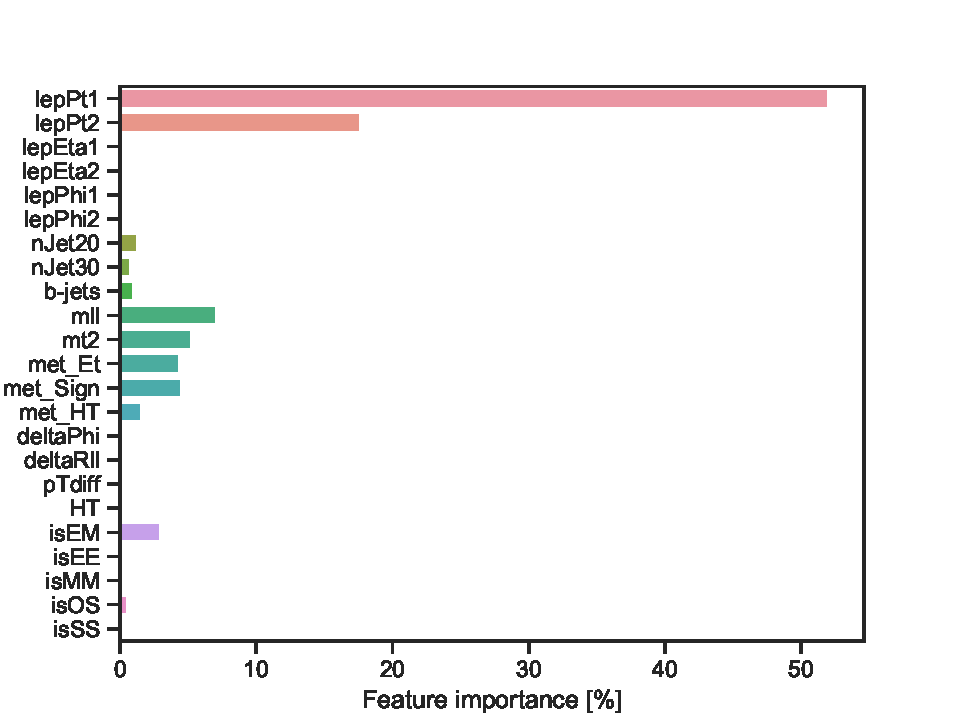
\includegraphics[width = \textwidth]{Figures/SlepSlep/ML/BDT/All_level/High/featureImportance.pdf}
        \caption{Direct slepton production.}
        \label{fig:featSlepslepHigh}
    \end{subfigure}
    \begin{subfigure}[t!]{0.49\textwidth}
        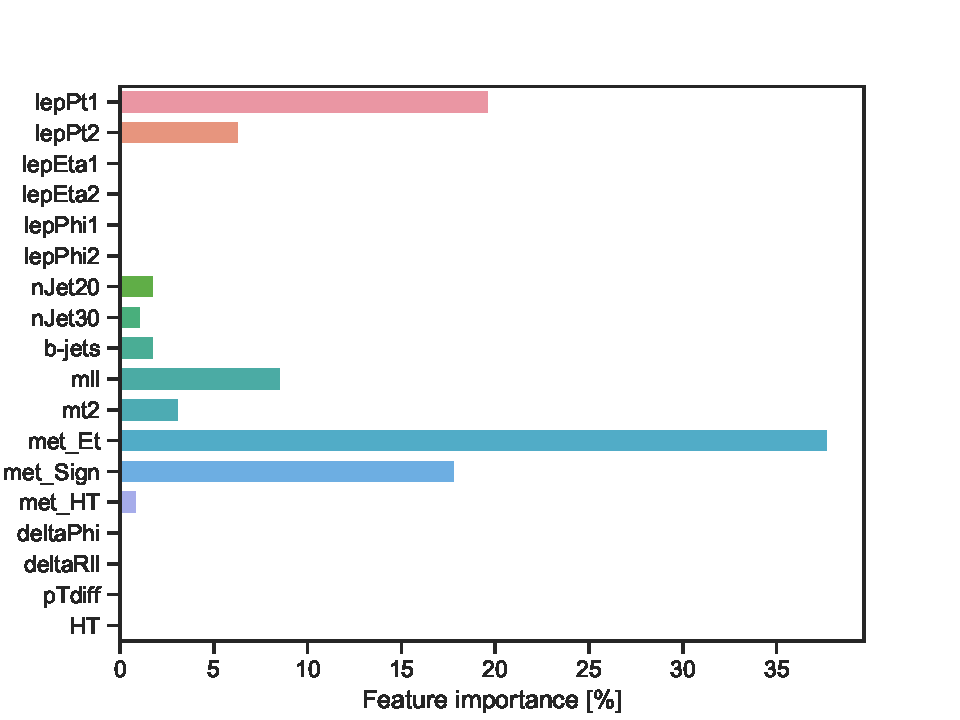
\includegraphics[width = \textwidth]{Figures/SlepSnu/BDT/All_level/High/featureImportance.pdf}
        \caption{Chargino production via $\Tilde{l}/\Tilde{\nu}$.}
        \label{fig:featSlepsnuHigh}
    \end{subfigure}
    \begin{subfigure}[t!]{0.49\textwidth}
        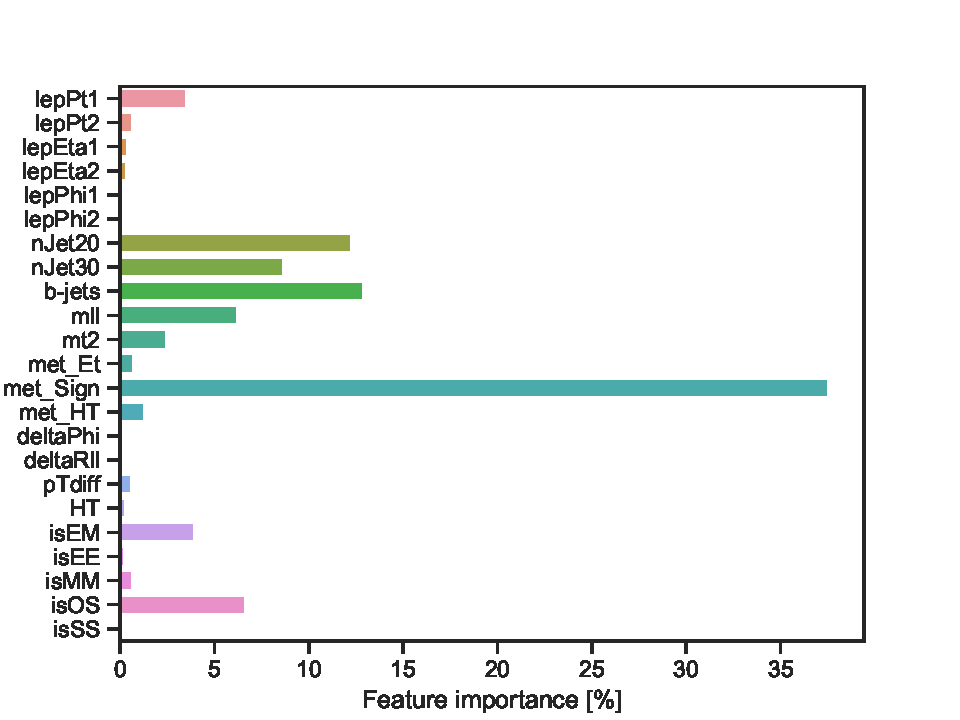
\includegraphics[width = \textwidth]{Figures/WW/BDT/All_level/High/featureImportance.pdf}
        \caption{Chargino production via $W^\pm$.}
        \label{fig:featWWHigh}
    \end{subfigure}
    \begin{subfigure}[t!]{0.49\textwidth}
        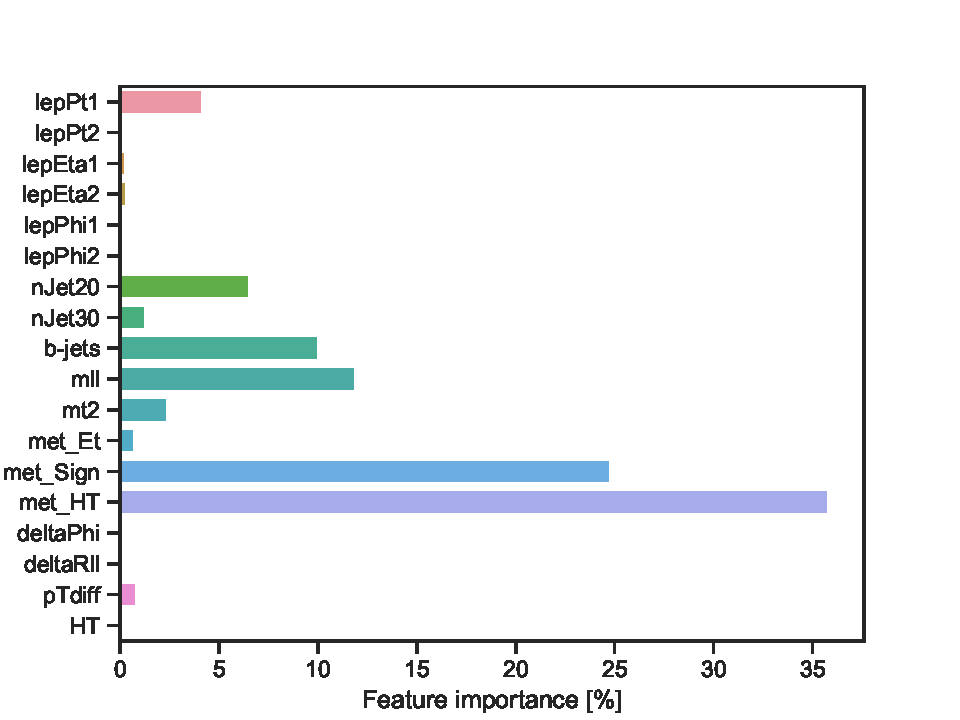
\includegraphics[width = \textwidth]{Figures/Mono_Z/ML/BDT/All_level/High/featureImportance.pdf}
        \caption{Mono-Z.}
        \label{fig:featMonoZHigh}
    \end{subfigure}
    \caption{Feature importance for high mass splittings for all four processes using all features during training.}
    \label{fig:AllHighfeatBDT}
\end{figure}

As we can see in figure \ref{fig:AllHighfeatBDT}, the momentum for the leading lepton have become a lot more interesting for the BDT especially for the direct slepton production and chargino production with slepton/sneutrino-mediated-decay. In addition the momentum for the subleading lepton have also gotten interesting for the two processes including sleptons. The rest of the features seems to be recurring for the processes no matter what mass splitting we look at. 



\begin{figure}[H]
    \centering
    \begin{subfigure}[t!]{0.49\textwidth}
        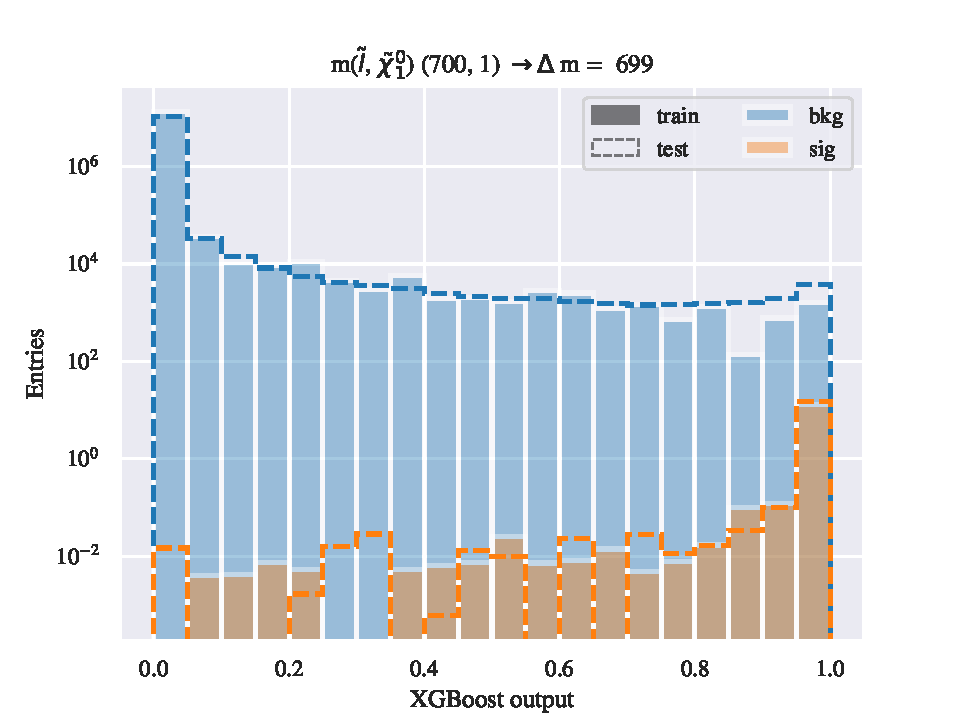
\includegraphics[width = \textwidth]{Figures/SlepSlep/ML/BDT/All_level/High/scaled_train_test_396033.pdf}
        \caption{Direct slepton production.}
        \label{fig:SlepslepHigh}
    \end{subfigure}
    \begin{subfigure}[t!]{0.49\textwidth}
        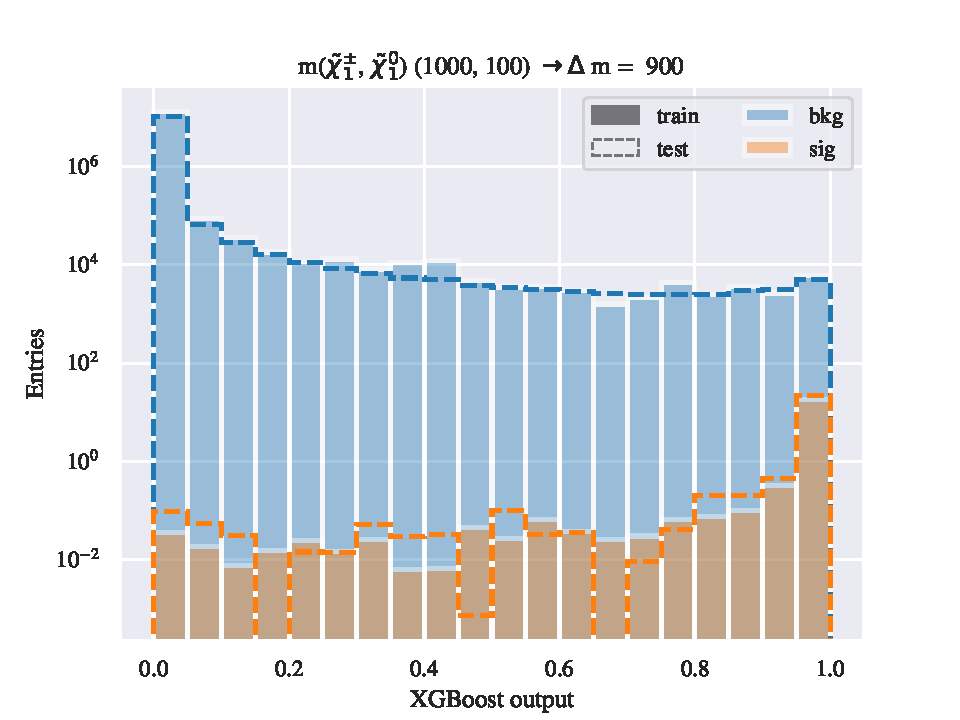
\includegraphics[width = \textwidth]{Figures/SlepSnu/BDT/All_level/High/scaled_train_test_397169.pdf}
        \caption{Chargino production via $\Tilde{l}/\Tilde{\nu}$.}
        \label{fig:SlepsnuHigh}
    \end{subfigure}
    \begin{subfigure}[t!]{0.49\textwidth}
        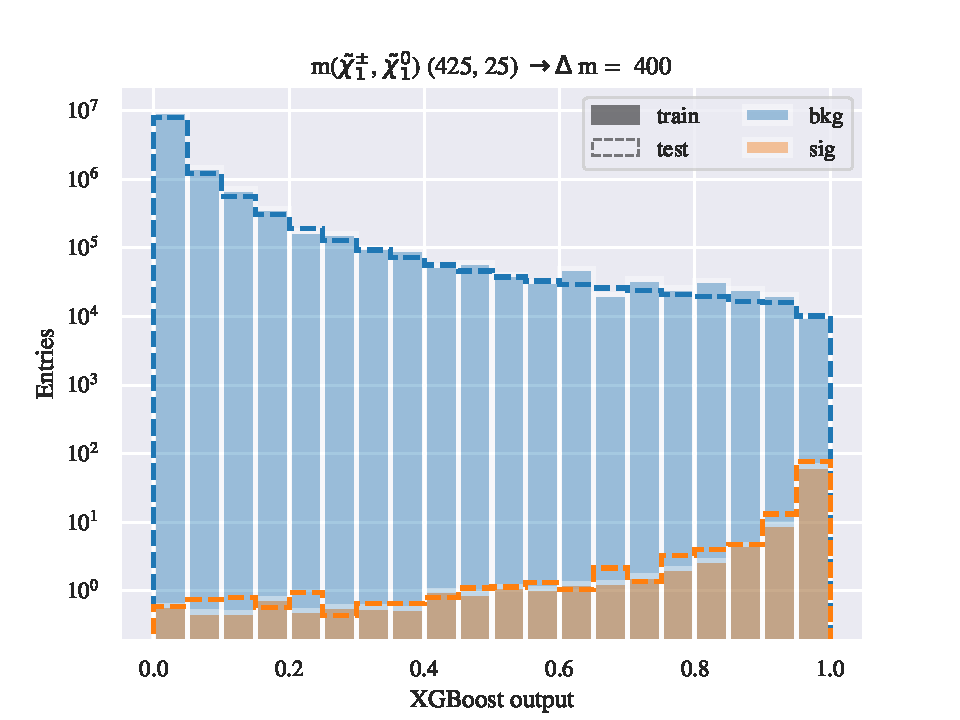
\includegraphics[width = \textwidth]{Figures/WW/BDT/All_level/High/scaled_train_test_395330.pdf}
        \caption{Chargino production via $W^\pm$.}
        \label{fig:WWHigh}
    \end{subfigure}
    \begin{subfigure}[t!]{0.49\textwidth}
        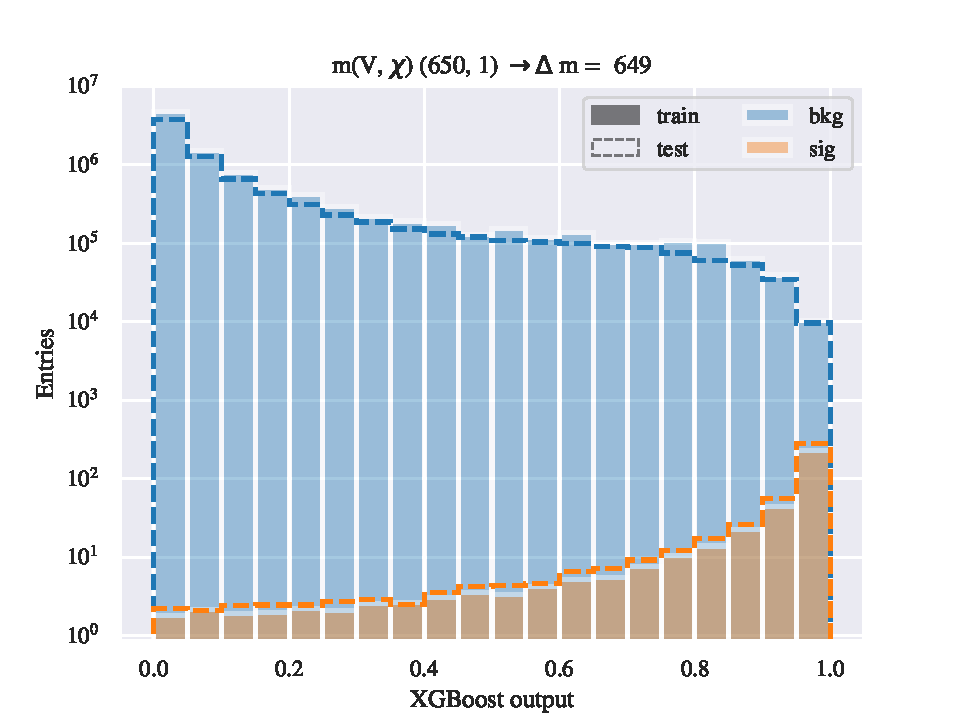
\includegraphics[width = \textwidth]{Figures/Mono_Z/ML/BDT/All_level/High/scaled_train_test_310617.pdf}
        \caption{Mono-Z.}
        \label{fig:MonoZHigh}
    \end{subfigure}
    \caption{Test vs train for high mass splittings done with the BDT. Here the test set is scaled up to match the number of training events.}
    \label{fig:AllHighBDT}
\end{figure}

In figure \ref{fig:AllHighBDT} we can see the results from testing our BDT. In figure \ref{fig:WWHigh} and \ref{fig:MonoZHigh} the match is overall pretty good between test and training, while for the processes in figure \ref{fig:SlepslepHigh} and \ref{fig:SlepsnuHigh} this does not match that well. It can be many reasons for this e.g. having too little input data to perform a proper training, the features that are chosen might be less efficient for the process with a given mass splitting or tendency to over/underfit. Nevertheless, it has succeeded in correctly classifying the signal and background to some extent. We can see for all four processes that we have more signal in the last bin than in any of the other models shown earlier in this chapter. This is of course not that surprising since these masses are outside of the SM masses we already know very well.



\section{Building, training and testing the Neural Network}
In the following sections we are going to look at how the Neural Network (NN) is built up, trained and tested before we in the end go to the last part of the ML where we are going to test both trained algorithms on real data.

\subsection{Building}
As for the BDT, the NN uses some already existing libraries. The main parts of the building is covered in chapter \ref{sec:NN} and the parameters we us to optimize the NN is presented in table \ref{tab:parametersNN}.

\begin{table}[H]
    \centering
    \renewcommand{\arraystretch}{1.}
    \begin{tabular}{c c}
    \toprule
        \textbf{Parameter} & \textbf{Value}\\
        \midrule
        \midrule
        Number of nodes & 300  \\
        Number of hidden layers & 5\\
        Dropout rate & 0\\
        Batch size & 32\\
        Epochs & 100000\\
        Learning rate & $10^{-5}$\\
        L1 & 0\\
        L2 & $10^{-3}$\\
        \bottomrule
    \end{tabular}
    \caption{An overview of the different parameters used during training to obtain the results for the NN.}
    \label{tab:parametersNN}
\end{table}

Most of the parameters are self explanatory, but we are going to go through them step by step so we are sure that we have understood every one of them. The first one is the number of nodes in each layer (and not the total number in the network). Then we have the number of hidden layers which is the number of layers we want inside the network in addition to the input and output layer. Dropout rate is a number between 0 and 1 and is taken into consideration if you want to drop a percentage of your input when you start training. As we can see, we have not used the dropout rate other than telling our NN that it should not drop any of the input events, so we are not discussing the advantages or disadvantages in using this here. The next parameter is the batch size which is the number of iterations we go through the data we give the NN. This can be any value above 1 but it is common to set it to a number of power of 2. The epochs and learning rate should be clear from chapter \ref{sec:NN}, where the epochs is not a very interesting parameter due to the early stopping and the learning rate gets optimized by Adam. The last two parameters we have to take into consideration are L1 and L2, which is what we call \textit{layer weight regularizes}. These are applied to add a penalty on the layers kernel and are simply added as a term in the cost/loss function in equation \ref{eq:loss}.

In addition to the parameters, we have to give our network an activation function for each layer in the network. In chapter \ref{sec:ML} we looked at different activation functions, where we have used two of them in our network, namely ReLU and Sigmoid. We have given the hidden layers ReLU as activation function and Sigmoid is only used for the output layer. 

As for the BDT, we have different compositions of mass splittings and features in the different NNs as well. 

\subsection{Training}
The training of the NN is the most time consuming step of all of the ML done in this thesis. It uses more time on solving the same problem as the BDT, which is one of the disadvantages of the NN compared to the BDT. The advantage is that the NN can do a better job than the BDT if we are able to choose the right parameters for training. Since the training of the NN takes some time, we have chosen to give it a patience of only 10 steps, instead of 20. After some trial and error during the work with this thesis we have concluded that when the network has not improved in 10 steps, it will not improve much more after 20 either. So after 10 steps, the early-stopping will come in and stop the training and save the model at the best epoch. 

\subsection{Testing}
The next step is to test the NN on our test set. This is again done on the same signal samples we used in the cut and count analysis. The results are presented with all four processes together with low, intermediate and high mass splittings and which set of features (low, high or all) performing best are evaluated by looking at the AUC-scores in table \ref{tab:AUCNN}.


\subsubsection{AUC-score}
In table \ref{tab:AUCNN}, we can see the AUC-score for each process and all combinations of mass splittings and features. There are several scores that are the same for the different features, but here we don't have the opportunity to look at the feature importance (because this is not relevant for NN) to make the decision. Instead we have chosen to show the same compositions as for the BDTs because the ones with the best score in NN are the same as with BDTs. 

\begin{table}[H]
    \centering
    \renewcommand{\arraystretch}{1.}
    \begin{tabular}{l l c c c c }
    \toprule
    \textbf{Level} & $\mathbf{\Delta m}$ & $\mathbf{\Tilde{l} \Tilde{l}}$ & $\mathbf{\Tilde{\chi}_1^\pm \rightarrow \Tilde{l}/\Tilde{\nu}}$ & $\mathbf{\Tilde{\chi}_1^\pm \rightarrow W^\pm}$ & \textbf{Mono-Z}  \\
    \midrule
    \midrule
    \multirow{3}{*}{High} &  Low   & 0.91 & 0.90 & 0.90 & 0.94 \\
     & Intermediate & 0.99 & 0.97 & 0.93 & 0.96 \\
     & High & 1.00 & 1.00 & 0.96 & 0.96 \\
     \midrule
    \multirow{3}{*}{Low} & Low & 0.96 & 0.93 & 0.93 & 0.96 \\
     & Intermediate & 0.99 & 0.98 & 0.95 & 0.97 \\
     & High & 1.00 & 1.00 & 0.97 & 0.97 \\
     \midrule
    \multirow{3}{*}{All} & Low & 0.97 & 0.94 & 0.94 & 0.96 \\
     & Intermediate & 1.00 & 0.98 & 0.96 & 0.97 \\
     & High & 1.00 & 1.00 & 0.97 & 0.98 \\
     \bottomrule
    \end{tabular}
    \caption{The AUC score for the different processes trained on different compositions of features and mass splittings for the NN.}
    \label{tab:AUCNN}
\end{table}







\subsubsection{Low mass splittings}
The first results from the NN we are going to look at are the ones with low mass splittings and trained on all features. 

\begin{figure}[H]
    \centering
    \begin{subfigure}[t!]{0.49\textwidth}
        \includegraphics[width = \textwidth]{Figures/SlepSlep/ML/NN/All_level/Low/scaled_train_test_395984.pdf}
        \caption{Direct slepton production.}
        \label{fig:SlepslepNNLow}
    \end{subfigure}
    \begin{subfigure}[t!]{0.49\textwidth}
        \includegraphics[width = \textwidth]{Figures/SlepSnu/NN/All_level/Low/scaled_train_test_397115.pdf}
        \caption{Chargino production via $\Tilde{l}/\Tilde{\nu}$.}
        \label{fig:SlepsnuNNLow}
    \end{subfigure}    
    \begin{subfigure}[t!]{0.49\textwidth}
        \includegraphics[width = \textwidth]{Figures/WW/NN/All_level/Low/scaled_train_test_395268.pdf}
        \caption{Chargino production via $W^\pm$.}
        \label{fig:WWNNLow}
    \end{subfigure}
    \begin{subfigure}[t!]{0.49\textwidth}
        \includegraphics[width = \textwidth]{Figures/Mono_Z/ML/NN/All_level/Low/scaled_train_test_310604.pdf}
        \caption{Mono-Z.}
        \label{fig:MonoZNNLow}
    \end{subfigure}
    \caption{Test vs train for low mass splittings with all features done with the NN. Here the test set is scaled up to match the number of training events.}
    \label{fig:AllLowNN}
\end{figure}

Figure \ref{fig:AllLowNN} shows a pretty good agreement between the test and training, but we don't have much signal for either of the four processes except for the chargino production processes, where we have been able to get more signal and less background towards 1.  













\subsubsection{Intermediate mass splittings}


The next results we are going to look at are from the model trained on intermediate mass splittings and all features, which are shown in figure \ref{fig:AllInterNN}.



\begin{figure}[H]
    \centering
    \begin{subfigure}[t!]{0.49\textwidth}
        \includegraphics[width = \textwidth]{Figures/SlepSlep/ML/NN/All_level/Inter/scaled_train_test_396014.pdf}
        \caption{Direct slepton production.}
        \label{fig:SlepslepNNInter}
    \end{subfigure}
    \begin{subfigure}[t!]{0.49\textwidth}
        \includegraphics[width = \textwidth]{Figures/SlepSnu/NN/All_level/Inter/scaled_train_test_397150.pdf}
        \caption{Chargino production via $\Tilde{l}/\Tilde{\nu}$.}
        \label{fig:SlepsnuNNInter}
    \end{subfigure}    
    \begin{subfigure}[t!]{0.49\textwidth}
        \includegraphics[width = \textwidth]{Figures/WW/NN/All_level/Inter/scaled_train_test_395320.pdf}
        \caption{Chargino production via $W^\pm$.}
        \label{fig:WWNNInter}
    \end{subfigure}
    \begin{subfigure}[t!]{0.49\textwidth}
        \includegraphics[width = \textwidth]{Figures/Mono_Z/ML/NN/All_level/Inter/scaled_train_test_310613.pdf}
        \caption{Mono-Z.}
        \label{fig:MonoZNNInter}
    \end{subfigure}
    \caption{Test vs train for low mass splittings with all features done with the NN. Here the test set is scaled up to match the number of training events.}
    \label{fig:AllInterNN}
\end{figure}

As for the BDT there is a good compliance between train and test with some fluctuations. What might be interesting in these results compared to the results in figure \ref{fig:AllLowNN} for low mass splittings, is that we actually got less signal towards one for intermediate mass splittings than we had for low. We would expect that this would be the other way around because of the bigger mass splittings between these particles.



















\subsubsection{High mass splittings}

The last trained NN we are looking at is the one trained on high mass splittings and all features. The results are presented in figure \ref{fig:AllHighNN}. 



\begin{figure}[H]
    \centering
    \begin{subfigure}[t!]{0.49\textwidth}
        \includegraphics[width = \textwidth]{Figures/SlepSlep/ML/NN/All_level/High/scaled_train_test_396033.pdf}
        \caption{Direct slepton production.}
        \label{fig:SlepslepNNHigh}
    \end{subfigure}
    \begin{subfigure}[t!]{0.49\textwidth}
        \includegraphics[width = \textwidth]{Figures/SlepSnu/NN/All_level/High/scaled_train_test_397169.pdf}
        \caption{Chargino production via $\Tilde{l}/\Tilde{\nu}$.}
        \label{fig:SlepsnuNNHigh}
    \end{subfigure}      
    \begin{subfigure}[t!]{0.49\textwidth}
        \includegraphics[width = \textwidth]{Figures/WW/NN/All_level/High/scaled_train_test_395330.pdf}
        \caption{Chargino production via $W^\pm$.}
        \label{fig:WWNNHigh}
    \end{subfigure}
    \begin{subfigure}[t!]{0.49\textwidth}
        \includegraphics[width = \textwidth]{Figures/Mono_Z/ML/NN/All_level/High/scaled_train_test_310617.pdf}
        \caption{Mono-Z.}
        \label{fig:MonoZNNHigh}
    \end{subfigure}
    \caption{Test vs train for low mass splittings with all features done with the NN. Here the test set is scaled up to match the number of training events.}
    \label{fig:AllHighNN}
\end{figure}

For high mass splittings we can see that we have less background in the last bin for all four processes, which makes sense since it should be easier to separate the signal from the background at these masses. We still have some fluctuations, especially in the signal test set, but overall it seems that the test sample is not too much affected of this. 







\subsection{Summarizing the ML performance}
\label{sec:summary_ML}
Before we move on to testing the trained ML algorithms on actual collected data from ATLAS, we are going to summarize the BDT and NN a bit. The BDT and NN in general perform well even though the separation of background and signal could have been improved. To discuss some of the problems that have occurred, we can see that some bins are partly or completely empty for the background training set. We suspect that this can come from the reduction of the MC set to match the number of signal events, where some of the background that probably should have been in these bins are taken out before training. The reduction of the MC set was necessary to train the ML methods to perform well. But, since the test set overall seems to be unaffected by this, we have chosen to leave it like this.

For the the different mass splittings, we have also experienced that the ML have found it, in some cases, hard to classify the signal as signal. It is not just the masses of the particles themselves. As we have mentioned earlier in this chapter, it might have something to do with the fact that the masses are close to or similar to the SM particle masses. If the mass differences in the decay are large, more phase space is available in the decay, which typically give larger momentum to the decay products - in case of SUSY and DM this means more MET. When the mass splitting approaches the W-mass, it is almost impossible to distinguish the direct slepton decay and a SM WW event (where each W decays to lepton+neutrino). That is why mass splittings around and below 100 GeV are extremely difficult since one has to fight with an almost irreducible background from WW. 











\section{Testing the BDT and NN on real data}

In this section we are going to see how the BDT and the NN perform on non-simulated data, which is an extra test to see how well they are trained. We will look at all three signal samples for each process together, where the background and data come from the ML model trained on high mass splittings. This is, of course, tested on the ML models trained on low and intermediate mass splittings as well. However, exactly which trained model we use for the comparison of background and data did not have a big impact and therefore we have chosen to rather show all signals together for a better comparison. 

First we are going to look at the results from the BDT which are presented in figure \ref{fig:BDTdataAll}, where we have stacked the different backgrounds to see how much each contribute in different areas. 
%\newgeometry{twoside,inner=3cm,outer=2cm}
\begin{figure}[H]
    \centering
    \begin{subfigure}[t!]{0.49\textwidth}
        \includegraphics[width = \textwidth]{Figures/Stacked/stackedplot_BDT_All_level_slepslep.pdf}
        \caption{Direct slepton production.}
        \label{fig:BDTdataAllSlepSlep}
    \end{subfigure}
    \begin{subfigure}[t!]{0.49\textwidth}
        \includegraphics[width = \textwidth]{Figures/Stacked/stackedplot_BDT_All_level_slepsnu.pdf}
        \caption{Chargino production via $\Tilde{l}/\Tilde{\nu}$.}
        \label{fig:BDTdataAllSlepsnu}
    \end{subfigure}      
    \begin{subfigure}[t!]{0.49\textwidth}
        \includegraphics[width = \textwidth]{Figures/Stacked/stackedplot_BDT_All_level_WW.pdf}
        \caption{Chargino production via $W^\pm$.}
        \label{fig:BDTdataAllWW}
    \end{subfigure}
    \begin{subfigure}[t!]{0.49\textwidth}
        \includegraphics[width = \textwidth]{Figures/Stacked/stackedplot_BDT_All_level_monoZ.pdf}
        \caption{Mono-Z.}
        \label{fig:BDTdataAllmonoZ}
    \end{subfigure}
    \caption{The output from the test set together with real data using BDTs. Here the different backgrounds are stacked to see how much they contribute together with the three benchmark signals for each process.}
    \label{fig:BDTdataAll}
\end{figure}
%\restoregeometry

In figure \ref{fig:BDTdataAll}, we can see that the data and background have a pretty good compliance with some minor fluctuations, which might be caused by the weights for each event. Some of the events have gotten negative weights when we have multiplied them together, but since the differences are well within $\pm$20\%, we have not considered this as a problem. We can also see that there are some fluctuations in the different background contributions in the bins, but since we are looking at around 30\% of the MC background we have to expect some statistical fluctuations. This seems not to affect overall the performance, however, which means that we can trust the results we have obtained. 

It might be a bit difficult to see because of the logarithmic scale, but in the last bin we have most contribution from dibosons. This is a very good sign because this background is the one that looks most like the signature in question and suggests that the BDT handles the different background contributions well. This can also be drawn back to the cut and count analysis, where the diboson background definitely is the dominating background after applying all cuts. 

We have also tested the NN on data which are presented in figure \ref{fig:NNdataAll}.

%\newgeometry{twoside,inner=3cm,outer=2cm}
\begin{figure}[H]
    \centering
    \begin{subfigure}[t!]{0.49\textwidth}
        \includegraphics[width = \textwidth]{Figures/Stacked/stackedplot_NN_All_level_slepslep.pdf}
        \caption{Direct slepton production.}
        \label{fig:NNdataAllSlepSlep}
    \end{subfigure}
    \begin{subfigure}[t!]{0.49\textwidth}
        \includegraphics[width = \textwidth]{Figures/Stacked/stackedplot_NN_All_level_slepsnu.pdf}
        \caption{Chargino production via $\Tilde{l}/\Tilde{\nu}$.}
        \label{fig:NNdataAllSlepSnu}
    \end{subfigure}      
    \begin{subfigure}[t!]{0.49\textwidth}
        \includegraphics[width = \textwidth]{Figures/Stacked/stackedplot_NN_All_level_WW.pdf}
        \caption{Chargino production via $W^\pm$.}
        \label{fig:NNdataAllWW}
    \end{subfigure}
    \begin{subfigure}[t!]{0.49\textwidth}
        \includegraphics[width = \textwidth]{Figures/Stacked/stackedplot_NN_All_level_monoZ.pdf}
        \caption{Mono-Z.}
        \label{fig:NNdataAllmonoZ}
    \end{subfigure}
    \caption{The output from the test set together with real data from the NN. Here the different backgrounds are stacked to see how much they contribute together with the three benchmark signals for each process.}
    \label{fig:NNdataAll}
\end{figure}
%\restoregeometry

When comparing the results for the BDT and the results for the NN in figure \ref{fig:BDTdataAll} and \ref{fig:NNdataAll}, we cannot see much differences except for a couple of fluctuations in the different background contributions. The data and the MC seem to have a good compliance and diboson is the dominating background where we expect to have most of our signal.

It looks like our BDT and NN do a good job in separating the signal and background, and it handled the real data very well as well. The next and last step in this thesis is to check if our models are sensitive to actually discover new physics and compare the results from using ML with the results from the cut and count analysis. 






































\begin{comment}





These cuts are done in a script called \texttt{importdata.py} where you also set up all of the data (both MC and real data) in pandas dataframes \footnote{Pandas dataframes \cite{PD} is a two-dimensional frame of your data which also includes the corresponding labels.}. In this script you will find a function called \texttt{prepareInput} which will read in all of the data in chunks because reading in all of it at once is too much for the computer to handle. After reading in one chunk, the root files will be set up in Pandas dataframes before it is sent into the precuts function called \texttt{importData}. Then we shuffle all of the events in each chunk before we send it in to the function called \texttt{selectFeatures} where we select the features we want to have for our training in the ML algorithm. The features I chose for the direct slepton production is given in table \ref{tab:features}.



The next step is to get the event weights in the function \texttt{getEventWeights} where we weight each event depending on the different weights listed in table \ref{tab:eventWeights} and the luminosity which is 58.5 fb$^{(-1)}$ in our case.



And in the end it stores the preprocessed data in HDF5 files before it starts on a new chunk and do the process described above continuously until we have reached the end of the dataset. HDF5 \cite{hdf5} is a file format to store large, complex and heterogeneous data which we use to store our events temporarily to save some time so we don't have to do this part every time we are training a ML model. This is also a time consuming step of the code. All of this can be run by simply running \texttt{main.py} with some arguments. If you are going to do the preprocessing you can add \texttt{--prepare\_hdf5} as argument and if you want to do it for signal (\texttt{--sig}), background (\texttt{--bkg}) and data (\texttt{--data}). I have also divided the signal samples into low, intermediate and high mass splitting to get more statistics from the training and testing. This means if you are going to do this for signal you have to add an argument \texttt{--low}, \texttt{--inter} or \texttt{--high}, where low is $\Delta m < 100$GeV, intermediate is $100$GeV $\leq \Delta m < 450$GeV and high is $\Delta m \geq 450$GeV. Which signal samples that are in which "group", you can see in table \ref{tab:directslepLOW}, \ref{tab:directslepINTER1}, \ref{tab:directslepINTER2} and \ref{tab:directslepHIGH} in section \ref{sec:sigsamptab}.

The next step is to do the actual ML which can be done by running the script \texttt{main.py} with some new arguments. The first thing you want to do is to read in the HDF5 files we made in the previous part which is simply done by adding \texttt{--read\_hdf5} as an argument. You also have to choose if you wanna train the model on low, intermediate mass splitting which is done by adding \texttt{--sig} and one of the following arguments \texttt{--low}, \texttt{--inter} or \texttt{--high}. You also have to choose which model you wanna train where you add either \texttt{--xgboost} for running XGBoost or \texttt{--nn} to run the neural network. If you run with all of this arguments you will train a new model. If you don't want to train a new model and just use a earlier trained model you can simply add \texttt{--load\_pretrained\_model} and it will use a pretrained model instead. This is mostly used to see how our model are doing compared to real data. To do this you have to read the hdf5 files, load the pretrained model, tell if you want the low, intermediate or high version and that you want data, which is done by simply adding the argument \texttt{--data}. 


\end{comment}










\begin{comment}



\begin{figure}[H]
%\begin{minipage}{2\textwidth}
%\begin{adjustwidth}{-3cm}{-3cm}
\centering
%\advance\leftskip-4cm 
%\advance\rightskip-4cm 
    \begin{subfloat}[][a]
        \includegraphics{Figures/SlepSlep/CutAndCount/ML_cuts/hist1d_mll_ML_cuts.pdf}
    \caption{Invariant mass.}
    \label{fig:my_label}
    \end{subfloat}
    \begin{subfloat}[t!]{0.49\textwidth}
        \includegraphics[width=\textwidth]{Figures/SlepSlep/CutAndCount/ML_cuts/hist1d_met_Et_ML_cuts.pdf}
    \caption{Missing transverse energy.}
    \label{fig:my_label}
    \end{subfloat}
    \\
    \begin{subfloat}[t!]{0.49\textwidth}
        \includegraphics[width=\textwidth]{Figures/SlepSlep/CutAndCount/ML_cuts/hist1d_mt2_ML_cuts.pdf}
    \caption{Stransverse mass.}
    \label{fig:my_label}
    \end{subfloat}
    \begin{subfloat}[t!]{0.49\textwidth}
        \includegraphics[width=\textwidth]{Figures/SlepSlep/CutAndCount/ML_cuts/hist1d_nBJet20_MV2c10_FixedCutBEff_77_ML_cuts.pdf}
    \caption{B-jets.}
    \label{fig:my_label}
    \end{subfloat}
    \\
    \begin{subfloat}[t!]{0.49\textwidth}
        \includegraphics[width=\textwidth]{Figures/SlepSlep/CutAndCount/ML_cuts/hist1d_nJet20_ML_cuts.pdf}
    \caption{Jets with $p_T > 20$GeV.}
    \label{fig:my_label}
    \end{subfloat}
    \begin{subfloat}[t!]{0.49\textwidth}
        \includegraphics[width=\textwidth]{Figures/SlepSlep/CutAndCount/ML_cuts/hist1d_nJet30_ML_cuts.pdf}
    \caption{Jets with $p_T > 30$GeV.}
    \label{fig:my_label}
    \end{subfloat}
    \\
    \begin{subfloat}[t!]{0.49\textwidth}
        \includegraphics[width=\textwidth]{Figures/SlepSlep/CutAndCount/ML_cuts/hist1d_lepPt[0]_ML_cuts.pdf}
    \caption{The transverse momentum for lepton 1.}
    \label{fig:my_label}
    \end{subfloat}
    \begin{subfloat}[t!]{0.49\textwidth}
        \includegraphics[width=\textwidth]{Figures/SlepSlep/CutAndCount/ML_cuts/hist1d_lepPt[1]_ML_cuts.pdf}
   \caption{The transverse momentum for lepton 2.}
   \label{fig:my_label}
    \end{subfloat}
    \\
    \begin{subfloat}[t!]{0.49\textwidth}
        \includegraphics[width=\textwidth]{Figures/SlepSlep/CutAndCount/ML_cuts/hist1d_lepPt_ML_cuts.pdf}
    \caption{The total transverse momentum for both leptons.}
    \label{fig:my_label}
    \end{subfloat}
    \begin{subfloat}[t!]{0.49\textwidth}
        \includegraphics[width=\textwidth]{Figures/SlepSlep/CutAndCount/ML_cuts/hist1d_pTdiff_ML_cuts.pdf}
    \caption{The absolute difference between the dilepton $p_T$, the selected jets $p_T$ and the vector sum of $\Vec{E}_T^{miss}$.}
    \label{fig:my_label}
    \end{subfloat}
    \\
    \begin{subfloat}[t!]{0.49\textwidth}
        \includegraphics[width=\textwidth]{Figures/SlepSlep/CutAndCount/ML_cuts/hist1d_deltaRll_ML_cuts.pdf}
    \caption{The distance between the two leptons.}
    \label{fig:my_label}
    \end{subfloat}
    \begin{subfloat}[t!]{0.49\textwidth}
        \includegraphics[width=\textwidth]{Figures/SlepSlep/CutAndCount/ML_cuts/hist1d_deltaPhi_ML_cuts.pdf}
    \caption{The azimuthal angle difference between the dilepton system and $E_T^{miss}$.}
    \label{fig:my_label}
    \end{subfloat}
\end{figure}

\begin{figure}[H]
%\begin{minipage}{2\textwidth}
%\begin{adjustwidth}{-3cm}{-3cm}
\centering
    \begin{subfigure}[t!]{0.49\textwidth}
        \includegraphics[width=\textwidth]{Figures/SlepSlep/CutAndCount/ML_cuts/hist1d_HT_ML_cuts.pdf}
    \caption{The scalar sum of the $p_T$ of the selected jets and leptons.}
    \label{fig:my_label}
    \end{subfigure}
    \begin{subfigure}[t!]{0.49\textwidth}
        \includegraphics[width=\textwidth]{Figures/SlepSlep/CutAndCount/ML_cuts/hist1d_met_HT_ML_cuts.pdf}
    \caption{}
    \label{fig:my_label}
    \end{subfigure}
    
%\end{adjustwidth}
\end{figure}


\end{comment}





















